\documentclass[16pt,a4paper,openany,twoside]{book}

\usepackage[pdftex]{graphicx}
\usepackage{caption}
\usepackage{subcaption}
\usepackage[top=1in, bottom=1in, left=1.5in, right=1in]{geometry}
\usepackage{setspace}
\usepackage{tocbibind}
\usepackage{lineno}
\usepackage{definitions}
\usepackage[nomain,acronym,toc,nopostdot,nonumberlist]{glossaries}
\usepackage[pdftex,pdftitle={Dissertation},pdfauthor={John Garland Wood}]{hyperref}
\usepackage{chngpage} 

\author{John Garland Wood}

\makeglossaries
\newacronym{sm}{SM}{Standard Model}
\newacronym{bsm}{BSM}{Beyond the Standard Model}

\newacronym{cern}{CERN}{European Center for Nuclear Research}
\newacronym{lhc}{LHC}{Large Hadron Collider}
\newacronym{atlas}{ATLAS}{A Toroidal LHC Apparatus}
\newacronym{cms}{CMS}{Compact Muon Solenoid}
\newacronym{ecal}{ECAL}{Electromagnetic Calorimeter}
\newacronym{hcal}{HCAL}{Hadronic Calorimeter}

\newacronym{qft}{QFT}{Quantum Field Theory}
\newacronym{qed}{QED}{Quantum Electrodynamics}
\newacronym{qcd}{QCD}{Quantum Chromodynamics}
\newacronym{lo}{LO}{Leading Order}
\newacronym{nlo}{NLO}{Next to Leading Order}
\newacronym{isr}{ISR}{Initial State Radiation}
\newacronym{fsr}{FSR}{Final State Radiation}

\newacronym{mva}{MVA}{Multi-Variate Analysis}
\newacronym{ann}{ANN}{Artificial Nueral Network}
\newacronym{mlp}{MLP}{Multi-Layer Perceptron}
\newacronym{cfmlp}{CFMLP}{Cleinman-Freidman Multi-Layer Perceptron}
\newacronym{bdt}{BDT}{Boosted Decision Tree}

\newacronym{jhep}{JHEP}{Journal of High Energy Physics}

\global\def\@title{The Search for Higgs Boson Production in Association with a Top-Quark Pair in $pp$ Collisions at $\sqrt{s}$ = 8 TeV in the Lepton Plus Jets Final State}
\title{\@title}

\begin{document}
%%\setlength{\parindent}{1cm}

\frontmatter
\begin{titlepage}
  \centering
  \doublespacing
  
  \vspace*{0.5in}
  \textbf{\Large \@title}\\[0.75in]
  Brian Patrick Francis\\
  Charlottesville, VA\\[0.5in]
  B.S., The University of Massachusetts Amherst, 2009\\[1.5in]
  A Dissertation presented to the Graduate Faculty\\
  of the Unversity of Virginia in Candidacy for the Degree of\\
  Doctor of Philosophy\\[0.5in]
  Department of Physics\\[0.5in]
  University of Virginia\\
  May, 2015\\

\end{titlepage}
\doublespacing
\begin{center}

\textbf{\Large Abstract}\\[0.25in]

\end{center}

\par The most important goal of the \acrfull{lhc} is to elucidate the mechanism of electroweak symmetry breaking.  The \acrfull{sm} Higgs boson is thought to be a prime candidate for this.  The newly discovered boson announced on July 4th, 2012, with a mass of ${\sim}125$~\GeVcc, has so far been shown to be consistent with a \acrshort{sm} Higgs.  However, the final confirmation of this new particle as the \acrshort{sm} Higgs depends on subsequent measurements of all of its properties.  The observation of this new particle in association with top-quark pairs would allow the couplings of this particle to top and bottom quarks to be directly measured. ~\ttH, with Higgs decaying to~\bbbar~is an excellent channel to explore due to the dominant branching ratio of Higgs to~\bbbar~and  the kinematic handle the~\ttbar~system offers on the event.  However, it presents a plethora of difficult challenges due to a low signal to background ratio and uncertainties on kinematically similar \acrshort{sm} backgrounds.  This work discusses the search for Higgs boson production in association with a top-quark pair in~\pp~collisions at $\sqrt{s}$ = 8~\TeV, collected by the \acrfull{cms} experiment at the \acrshort{lhc}.  The search has been performed and published in two stages.  The first analysis used the first 5.1~\fbinv, and was followed up by the second analysis with the full 2012 dataset, using a total integrated luminosity of 19.5~\fbinv     


\def\signrule{\vskip 0.75in\hbox{\vrule width 3.5in height 0.4pt \hskip 0.3in
 \vrule width 2in height 0.4pt}}

\newpage

\vbox{
  \thispagestyle{empty}
  \begin{singlespace}
    \hbox{We approve the dissertation of John Garland Wood.}
    \vskip 0.35in 
    \hbox{\null\hskip 3.9in Date of Signature}
    \signrule
    \raggedright\begin{tabular}{l}Supervisor: Prof. Christopher Neu\end{tabular}\par
    \vskip -0.2in
    \signrule
    \raggedright\begin{tabular}{l}Committee Member: Prof. Hank Thacker\end{tabular}\par
    \vskip -0.2in
    \signrule
    \raggedright\begin{tabular}{l}Committee Member: Prof. Edward Murphy\end{tabular}\par
    \vskip -0.2in
    \signrule
    \raggedright\begin{tabular}{l}Committee Member: Prof. Bradley Cox\end{tabular}\par
    %\raggedright\begin{tabular}{l}Committee Member: Prof. Bradley Cox\end{tabular}\par
    \vskip 0.75in
    \signrule
    %\raggedright\begin{tabular}{l}PhD Committee Chair: Prof. Bradley Cox\end{tabular}\par
    \raggedright\begin{tabular}{l}PhD Committee Chair: Prof. Craig Group\end{tabular}\par
    
  \end{singlespace}
} 
\newpage

\tableofcontents
\listoffigures
\listoftables
%\clearpage

\mainmatter
\linenumbers
\chapter{Introduction}
\label{introduction}

\begin{figure}
    \centering
    \begin{subfigure}[b]{0.3\textwidth}
        \label{fig:qft_lo_ee_scattering}
        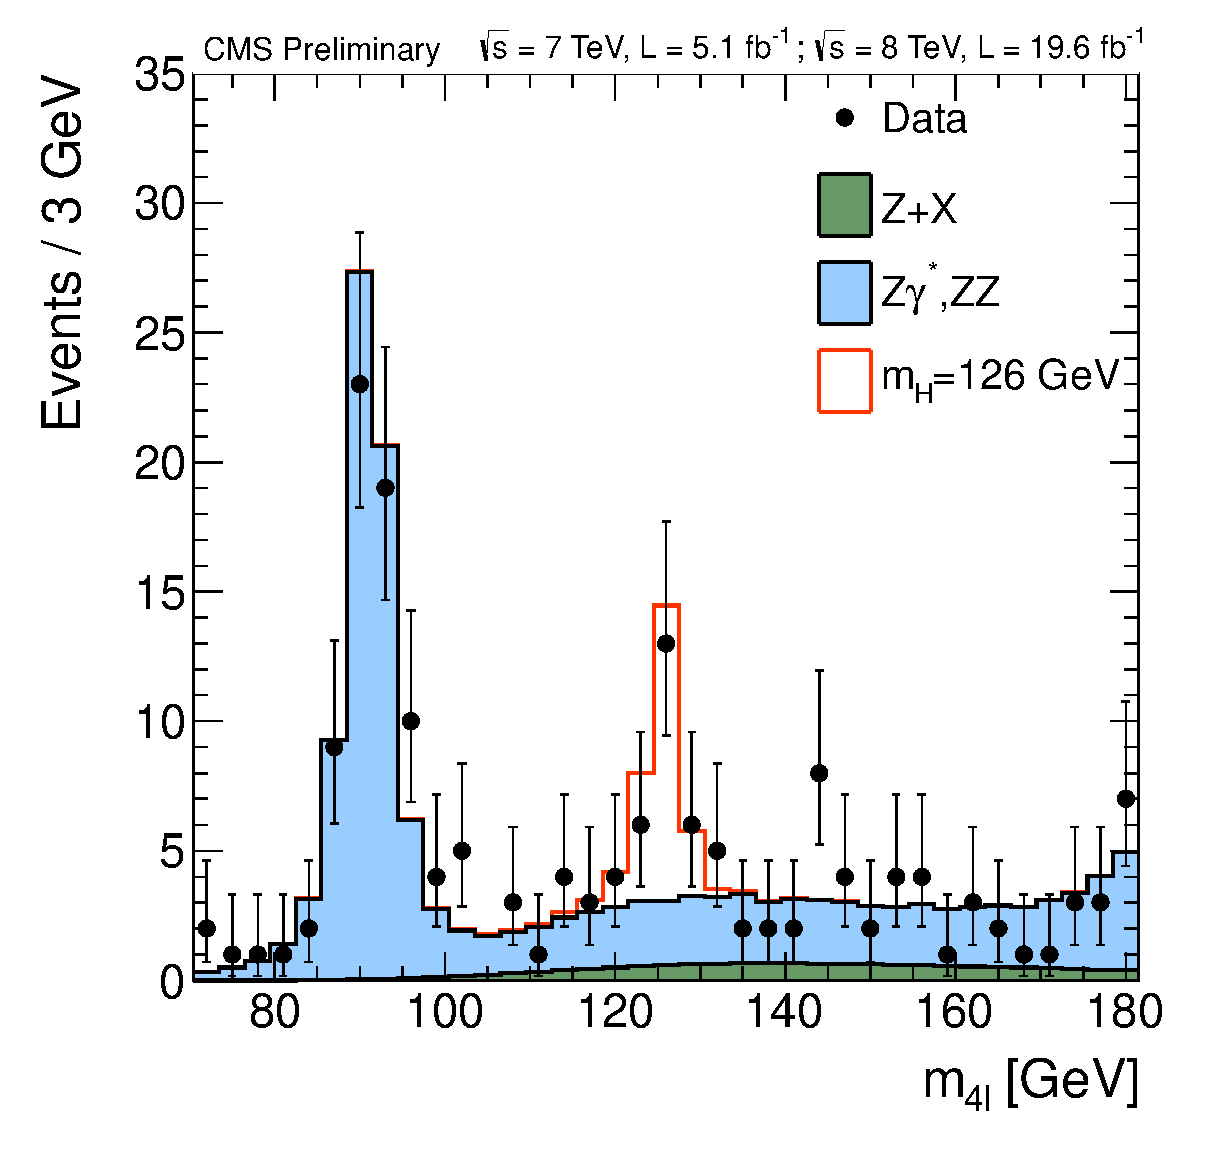
\includegraphics[width=\textwidth]{Figures/Experimental_Results/CmsHZZ4lMass.eps}
        \caption{CMS results for the $H\rightarrow~ZZ$ channel}
      \end{subfigure}
      ~ %add desired spacing between images, e. g. ~, \quad, \qquad, \hfill etc.
      % (or a blank line to force the subfigure onto a new line)
      \begin{subfigure}[b]{0.3\textwidth}
          \label{fig:qft_nlo_ee_scattering}
          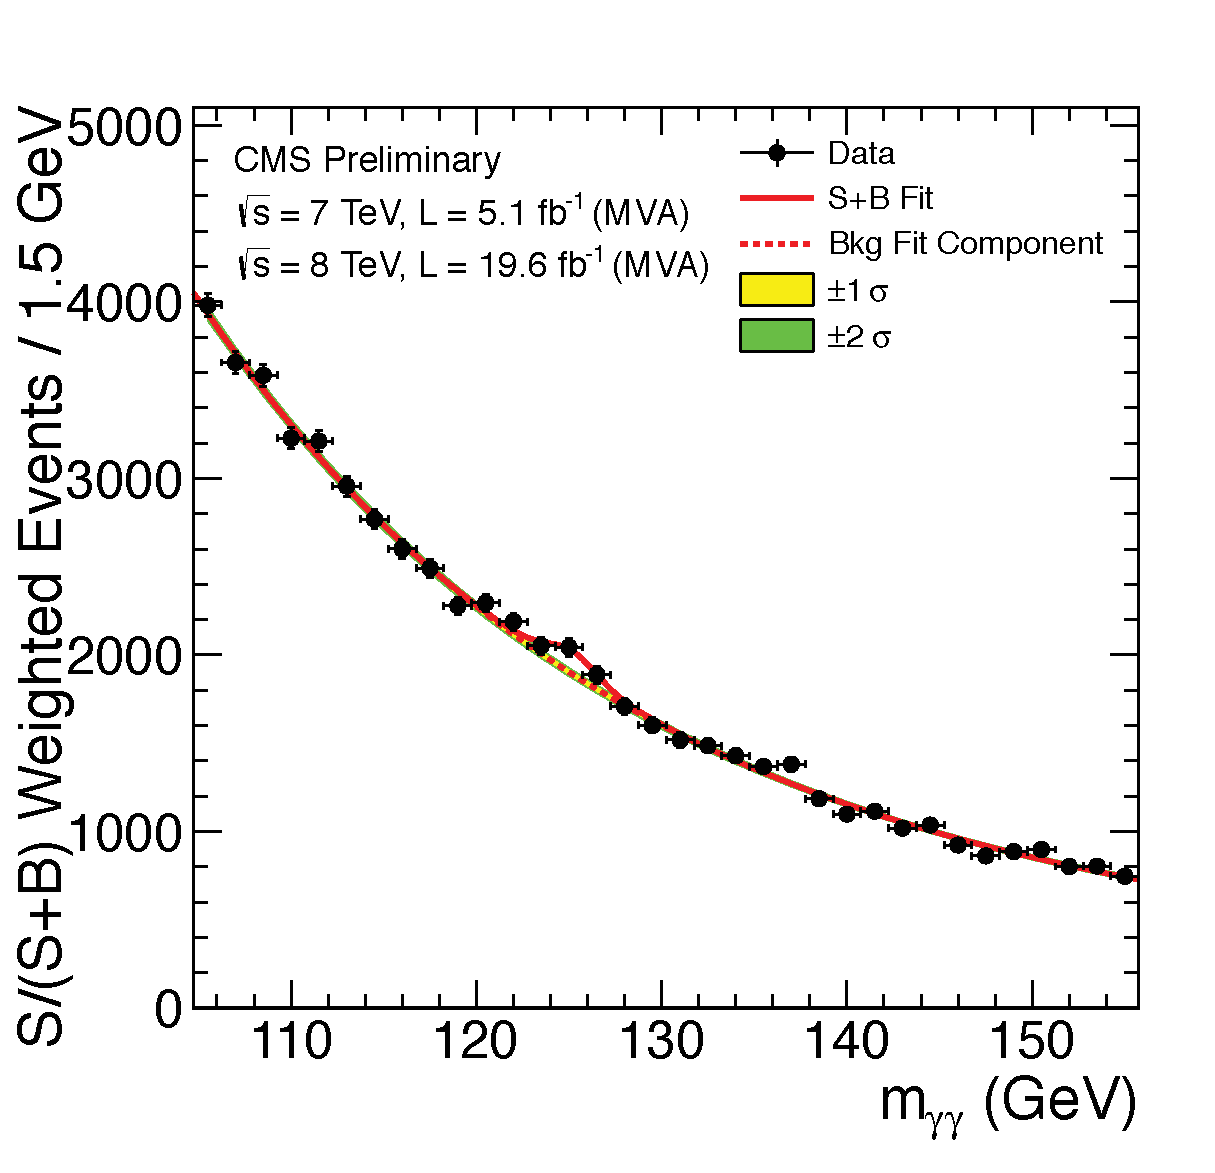
\includegraphics[width=\textwidth]{Figures/Experimental_Results/CmsHggMassMVAMoriond13.eps}
          \caption{CMS results for the $H\rightarrow\gamma\gamma$ channel}
      \end{subfigure}
      \caption{The CMS experiment has observed a new boson at m$\sim$125\GeVcc} \label{fig:cms_hZZ_hgg_results}
\end{figure}

\par On July 4th, 2012, the \acrfull{cms} and \acrfull{atlas} experiments announced the discovery of a new boson of mass $\sim~125$~\GeVcc~\cite{CMS:2012discovery}~\cite{ATLAS:2012discovery}.  The particle has been shown to be increasingly consistent with the description of the boson predicted by the Higgs mechanism of the \acrshort{sm}, as measurements on its mass, width, and quantum numbers are completed.  However, there are several properties of this new boson, which remain to be tested.  Figure \ref{fig:cms_hZZ_hgg_results} shows a consistent mass peak betwen the $H\rightarrow~ZZ$ and $H\rightarrow\gamma\gamma$ channels at the \acrshort{cms} experiment.  

\par The Yukawaka coupling of the Higgs boson to the top-quark in the \acrshort{sm} is the largest coupling among the fundamental particles and is well 
predicted - thus offering an excellent test of the nature of the coupling of the Higgs to fermions, as well as a potential probe into pysics \acrfull{bsm} that would alter this value from the \acrshort{sm} prediction.  The production of the Higgs boson in association with top-quark pairs is the best production mode at the \acrshort{lhc} that offers direct access to the top-Higgs coupling.  The dominant production mode of Higgs at the \acrshort{lhc}, gluon-gluon fusion, involves a triangle loop of strongly-coupled fermions, which includes all of the other quarks, as well as the potential for \acrshort{bsm} particles.  

\par ~\ttH~production also has the ability to constrain some extensions of the \acrshort{sm} that would not modify the Higgs branching fractions enough to be seen 
within current experiemental precision.  Such models include Little Higgs models, models with extra dimensions, top-color models, and compositie Higgs models that introduce a vector-like top partner, a $t'$, that can decay to $tH$, $bW$, or $tZ$ states.  Both $t't'$ and $t't$ production would produce a~\ttH~final state, or one that is indistinguishable from it ($tHbW$).  Upper limits on~\ttH~production would also provide limits on the previously described models, which would be complementary to existing direct searches for $t'$ particles, which attempt to reconstruct the $t'$ resonance.  

\par The~\ttH~channel has a rich set of possible final states.  Each top-quark will decay to a $b$-quark and a $W$ boson.  The $W$ boson will subsequently decay to two quarks, or a lepton and a neutrino.  These decays are classified as either hadronic, semi-leptonic, or di-leptonic for zero, one, or both $t$ quarks decaying leptonically 
respectively.  The Higgs may to decay to $b$-quark, $W$, $Z$, $\tau$, or $\gamma$ pairs.  In fact, this is one of the only production modes at the \acrshort{lhc} which 
has access to every Higgs decay mode, as other production mechanisms are swamped by large backgrounds preventing measurements of all Higgs decay types.  

\par The search is performed with the \acrshort{cms} experiment, a modern, general purpose particle detector capable of reconstructing and identifying hadronic jets, photons, electrons, muons, and tau leptons.  The hermetic design, and it's high precision and efficiency in reconstrucing and tracking every particle in a $pp$ collision, also makes it suitable for reconstructing missing transverse energy from the calculated momentum imbalance of all of the measured particles in the event.  This missing transverse energy is often the signature of a neutrino, which is the only \acrshort{sm} particle capable of escaping detection.  The detector uses a 3.8 T axial magnetic field, produced by the solenoid it is named after, to bend charged particles as they travel through the detector.  The measured curvature of their tracks allows the momentum of the particles to be calculated with to a high precision.  Tracks are formed and particles are reconstructed by a combination of sub-detector systems which work together to form the final final reconstructed image of each particle in the collision.  

\begin{figure}[h]
   \centering
  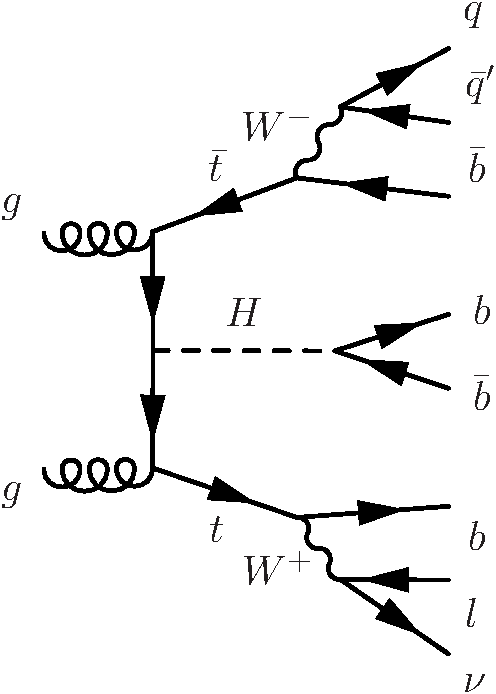
\includegraphics[width=0.5\textwidth]{Figures/Feynman_Diagrams/higgs_production__tth_semileptonic.pdf}
  \caption{A Feynman diagram of the~\ttH~process, with Higgs$\rightarrow$$b\bar{b}$, and the $t\bar{t}$-system decaying semi-leptonically} \label{fd:ttH_semiLep}
\end{figure}

\par This thesis will focus on a semi-leptonic decay of the top-quarks, with the Higgs decaying to a $b$-quark pair.  Figure \ref{fd:ttH_semiLep} is Feynman diagrm of the~\ttH~process.  The largest background to this process is top-quark pair production with extra jets originating from \acrfull{isr} or \acrfull{fsr} radiation,~\ttjets.  The irreducible background is formed by top-quark pairs, where a gluon is radiated and decays to $b$-quark pairs,~\ttbb.  In addition to the large backgrounds, the high jet multiplicity in the~\ttH~final state gives rise to a combinatorics problem in associating each jet with its role in the~\ttH~system.  This inevitably leads to misidentifying which jets are the decay product of the Higgs, and thus additionally smears out the resolution on the mass of the Higgs.  Due to the similarity of the~\ttbb~background and the combinatorics issue, no single variable is suitable for signal extraction.  A \acrfull{mva} technique is used in an attempt to isolate the~\ttH~signal from the~\ttjets background.  The \acrshort{mva} provides a one-dimensional discriminant based on several input variables related to the kinematics of the event.  This discrimant is then used to perform signal extraction and set upper-limits on~\ttH~ production.  The results of two searches will be presented.  The first result used the first 5.1~\fbinv of the 2012 dataset, with center of mass energy of 8~\TeV, and was published in the \acrfull{jhep}, May 2013.  The second result was update with the full 19.4~\fbinv 8~\TeV dataset, and was published in \acrshort{jhep}, Spetember 2014.   

\chapter{Theoretical Background}
\label{theoretical_background}

\par The \acrfull{sm} of particle physics represents the sum of
knowledge of the fundamental particles and their interactions with
each other.  It is a \acrfull{qft} that represents the interactions of each of the
fundamental forces through the symmetry of a mathematical object
known as a Lie group.  It is the theory that dictates the rate that
the~\ttH~process is produced, as well as the kinematics of every
particle involved.  As such, its predictions are critical for modeling
the charateristic signature of the~\ttH~signal in the \acrshort{cms}
detector, as well as the background processes, like~\ttbb~which leave
a kinematically similar final state signature.     


\section{An Overview of Quantum Field Theory}
\label{qft_overview}

\par \acrfull{qft} was developed out of the need for a
relativistic description of quantum mechanics.  Since the Einstein
relation $E=mc^{2}$ allows for the creation of particle-antiparticle
pairs, the single-particle description used in non-relativistic quantum
mechanics, fails describe this phenomenom~\cite{Peskin_Schroeder}.
This additionally fails when considering that Heisenberg's uncertainty
relation, $\Delta~E\cdot~\Delta~t = \hbar$, allows for an arbitrary
number of intermediate, virtual particles to be created.  By
quantizing a field representing a certain type of particle,
multiparticle states are naturally described as discreet excitations
of that field.  

% Lorentz invariance reveals a relationship between matter/antimatter
\par Lorentz invariance, and the need to preserve causality, also define a
fundamental relationship between matter and antimatter.  The
propagation of a particle across a space-like interval is treated
equivalently to the an anti-particle propagating in the opposite
direction~\cite{Peskin_Schroeder}.  This is done so that the net
probability amplitude for the particles to have an effect on a 
measurment occuring accross a space-like interval cancel each other,
thus preserving cuasality.  This cancellation requirement additionally
implies that the particle and anti-particle have the same mass, with
opposite quantum numbers such as spin or electric charge.   

% Accounting for spin 
\par The Lorentz transformations for a scalar field are different than
for a field with internal degrees of freedom, such as spin.  A
rotation on a vector field, will affect both its location, as well as
it's orentation~\cite{Peskin_Schroeder}.  This means the Lorentz
invariant equation of motion descirbing a scalar field will have a
different form than equations of motion for a field with spin.  The
most relevant equations describe the particles of \acrshort{sm}, which
contain spins of 0, 1/2, and 1.  They are described by the
Klein-Gordan, Dirac, and Proca equations respectively. \\

\noindent Klein-Gordon equation, for scalar (spin 0) fields 
\begin{equation}\label{eq:klein_gordon_eom}
(\partial^{2} + m^{2})\phi = 0  
\end{equation} 

\noindent Dirac equation, for spinor (spin 1/2) fields 
\begin{equation}\label{eq:dirac_eom}
(i\gamma^{\mu}\partial_{\mu} - m)\psi = 0 
\end{equation} 

\noindent Proca equation, for vector (spin 1) fields
\begin{equation}\label{eq:proca_eom}
\partial_{\mu}(\partial^{\mu}A^{\nu} - \partial^{\nu}A^{\mu}) + m^{2}A^{\nu}
= 0 
\end{equation} 

% From the free fields to interactions
\par With these equations, one can build a theory of free particles.
The Lagrangian formulation is the most appropriate since all
expressions are explicitly Lorentz invariant~\cite{Peskin_Schroeder}.
The Lagrangians for the Klein-Gordon, Dirac, and Proca equations are
given as: \\

\noindent Klein-Gordon Lagrangian, for real and complex scalar fields
\begin{equation}\label{eq:klein_gordon_lagrangian}
\begin{aligned}
& \mathcal{L} = \partial_{\mu}\partial^{\mu}\phi^{2} - \frac{1}{2}m^{2}\phi^{2}  \\
& \mathcal{L} = (\partial_{\mu}\phi)^{\ast}(\partial^{\mu}\phi) - m^{2}(\phi)^{\ast}(\phi) 
\end{aligned}
\end{equation}

\noindent Dirac Lagrangian, for spinor fields
\begin{equation}\label{eq:dirac_lagrangian}
\mathcal{L} = i\bar{\psi}\gamma^{\mu}\partial_{\mu}\psi - m\bar{\psi}\psi 
\end{equation}

\noindent Proca Lagrangian, for vector fields
\begin{equation}\label{eq:proca_lagrangian}
\mathcal{L} = -\frac{1}{4}F_{\mu\nu}F^{\mu\nu} + m^{2}A^{\nu}A_{\mu} 
\end{equation}

\noindent where $F_{\mu\nu}$, is the field strength tensor, defined as
$F_{\mu\nu} = \partial_{\mu}A_{\nu} - \partial{\nu}A_{\mu}$

\par Interactions are generated by coupling multiple fields together in a
single term, such as $ieA_{\mu}\bar{\psi}\psi$ and treating it as a
perturbation to the free field theory.  This implies every interaction
between particles is carried out by a virtual mediating particle.  When two
electrons scatter off one another, they are really exchanging a
virtual photon, the mediator of the electromagnetic force.  The
$W^{\pm} and Z$ bosons mediate the weak force, while the $gluons$
mediate the strong force.  

\begin{equation}\label{eq:lagrangian_free_interacting}
\mathcal{L} = \mathcal{L}_{Free} + \mathcal{L}_{Interacting}
\end{equation}

% Feynmann rules provide the method of calculating physical observables
\par In order to calculate the probability and dynamics of two
particles interacting with one another, an integral, constrained by
energy and momentum conservation, over the phase space of outgoing
particles and the scattering amplitude, $mathcal{M}$, is evaluated.
The scattering amplitude is calculated by using the propagtor (Green's
function of the free particle theory) for the incoming, mediating, and
outgoing particles, with an appropriate wieghting function, or vertex
factor, for each point the particles interact in the scattering
process, and then integrating over the momentum of the mediating
particle.  Richard Feynmann developed a set of rules for the writing
down the propagators and vertex factors directly from the Lagrangian,
and easily computing the scattering amplitude.  He also introduced an
elegant pictographic notation useful for visualizing particle
interactions, known as Feynmann diagrams. 

\begin{figure}
    \centering
    \begin{subfigure}[h]{0.45\textwidth}
        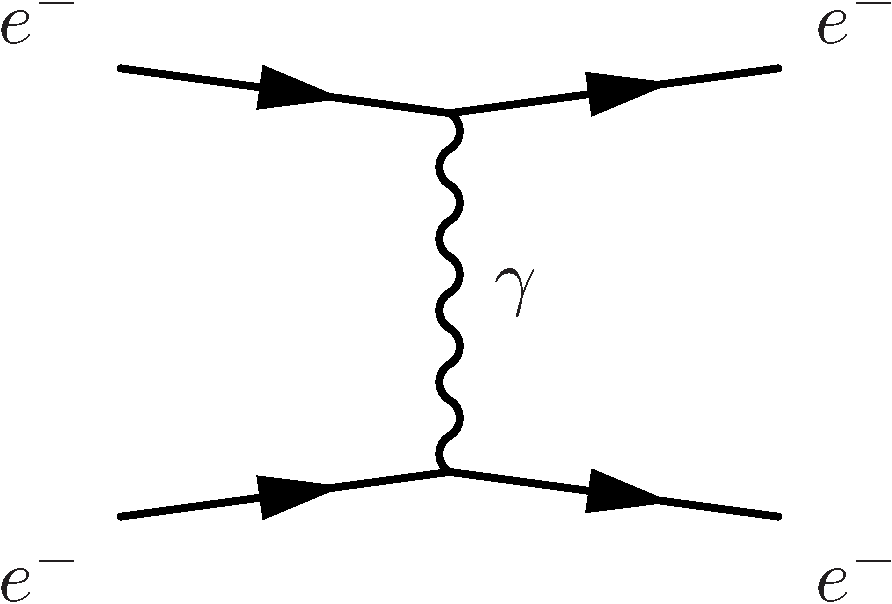
\includegraphics[width=\textwidth]{Figures/Feynman_Diagrams/qft_ex__lo_diagram__coulomb_scattering.pdf}
        \caption{A LO Feynman diagram }\label{fig:qft_lo_ee_scattering}
      \end{subfigure}
      ~ %add desired spacing between images, e. g. ~, \quad, \qquad, \hfill etc.
      % (or a blank line to force the subfigure onto a new line)
      \begin{subfigure}[h]{0.45\textwidth}
          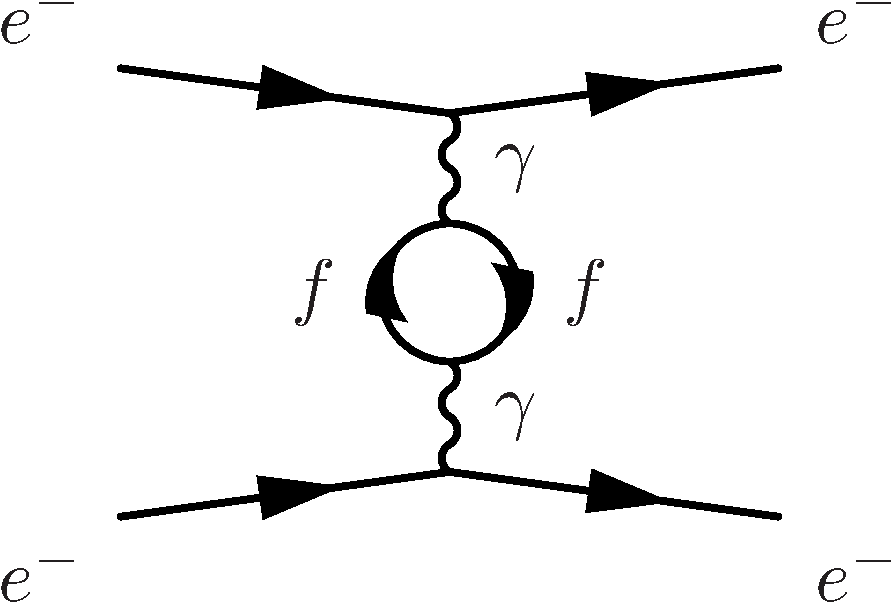
\includegraphics[width=\textwidth]{Figures/Feynman_Diagrams/qft_ex__nlo_diagram__coulomb_scattering.pdf}
          \caption{A NLO Feynman diagram}\label{fig:qft_nlo_ee_scattering}
      \end{subfigure}
      \caption{Leading and Next to Leading Order Feynman diagrams
        for the coulomb scattering process} \label{fig:feynman_diagrams_ee_scattering}
\end{figure}

\par With these tools, one can calculate the probability amplitudes of
a given process occuring to \acrfull{lo} without any
difficulties.  However, when calculations in \acrfull{nlo} are
performed, and loop diagrams of virtual particles are considered, the
probability amplitudes associated with a given process diverge to
infinity.  This occurs when one integrates over all of the 
possible momentum allowed by intermediate, loops of virtual particles,
which due to Heisenberg's uncertainty principle, are allowed to take
on any value of momentum.  Figure
\ref{fig:feynman_diagrams_ee_scattering} shows an example of a
\acrshort{lo} and \acrshort{nlo} process.

\begin{figure}[h]
  \centering
  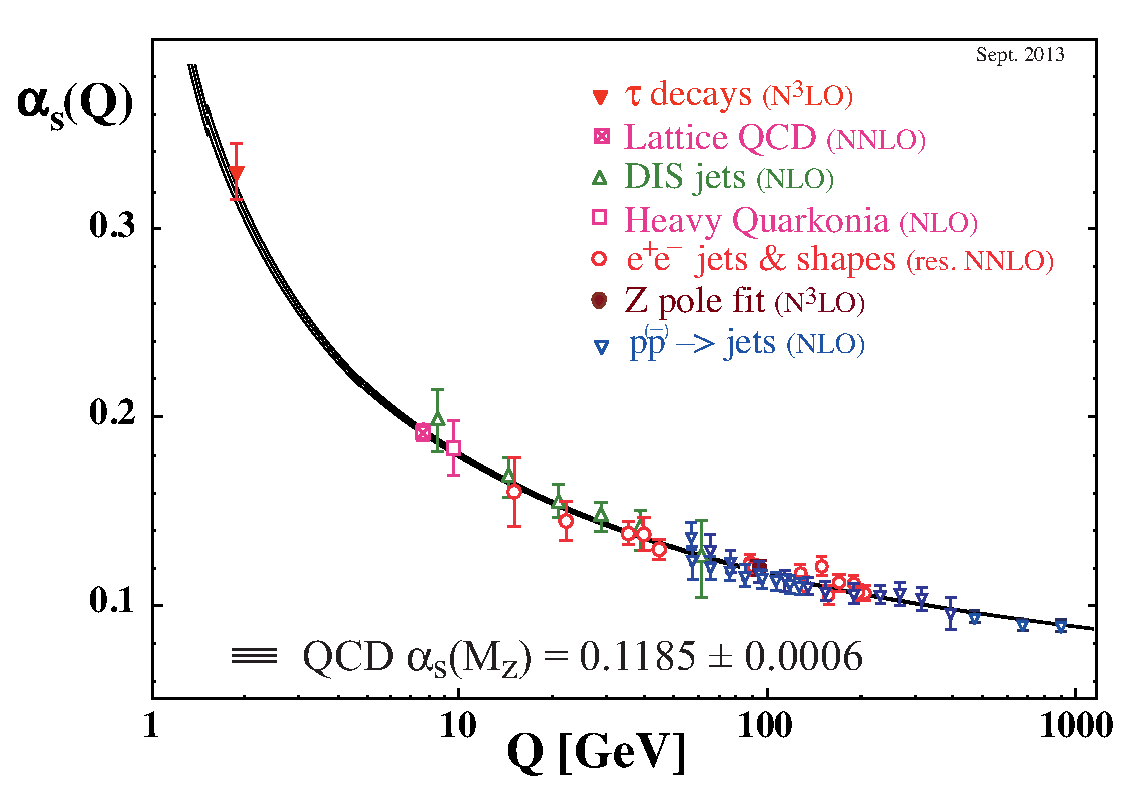
\includegraphics[width=0.5\textwidth]{Figures/Experimental_Results/asq-2013.eps}
  \caption{The global average of $\alpha_{s}$, the QCD coupling
    constant.}\label{fig:globalAvgAlphaS}
\end{figure}

\par The systematic removal of divergences from a theory is called
renormalization.  The divergences are absorbed into the
definitions of the free parameters of the theory, making the parameters a function of
the energy scale the process occurs at, instead of a constant.  This
allows for the calculations of fundamental processes to completed,
as long as the energy scale of the interaction is known.  A modern
interpretation of renormalization was provided by Kenneth
Wilson~\cite{th:Wilson_renormalization1}~\cite{th:Wilson_renormalization2}.
Instead of seeing the effects of high momentum calculations after
moving to \acrshort{nlo} in perturbation theory, one uses an effective Lagrangian,
computed by integrating out shells of momentum beginning at the energy
cutoff of the theory, where the \acrshort{nlo} effects begin the
dominate.  The dimensions of integration are then rescaled and the
result of evaluating the integral over the momentum shell is absorbed
into the definition of free parameters.  The processes is iterated
until the energy scale of the interaction is reached.  The functional 
dependence of the parameters is then  directly present in the resulting
effective Lagrangian, instead of appearing suddenly when accounting
for the one-loop contributions at \acrshort{nlo}.  Regardless of how
strange this procedure seem, the running of the coupling constant as a
function of interaction engergy has been validated experimentally time
and time and again, as shown in Figure \ref{fig:globalAvgAlphaS}~\cite{Bethke_WorldAvgAlphaS_QCD}.


\section{Abelian Gauge Theories of Particle Interactions}
\label{abelian_gauge_theory_overview}

\par In 1930, Herman Weyl introduced the idea that the interactions
between fields can be generated by requiring them to be invariant
under guage tansformations of a local symmetry~\cite{Weyl}.  For
electromagnetism, the local symmetry is that of the Lie group,
$U(1)$.  It is an abelian group, which has the property that the
generators of the group symmetry commutes with themselves. 
The $U(1)$ symmetry is invariant under phase rotations.  By requiring
local guage invariance, the Lagrangian must be unchanged under the 

\begin{equation}\label{eq:u1_psi_transformation}
\psi(x) \rightarrow e^{i\alpha(x)}\psi(x).
\end{equation}

Consider the Lagrangian for a free spin 1/2 particle: 

\begin{equation}\label{eq:dirac_lagrangian}
\mathcal{L} = \bar{\psi}(i\gamma^{\mu}\partial_{\mu} - m)\psi
\end{equation}

\noindent The first term in the Lagrangian, involving the derivative,
acts on $\alpha(x)$, creating a new term in the Lagrangian, breaking
its invariance under the local phase transformation.  

\begin{equation}\label{eq:u1_lagrangian_transformation}
\mathcal{L}\rightarrow\mathcal{L} -
(\partial_{\mu}\alpha)\bar{\psi}\gamma^{\mu}\psi
\end{equation}

\noindent Thus, a new term must be added to the orginial Lagrangian to cancel
out the term arising from the local phase transformation.  This is
achieved by defining the covariant derivative:

\begin{equation}\label{eq:covariant_derivative_em}
D_{\mu} = \partial_{\mu} + ieA_{\mu}
\end{equation} 

\noindent where $A_{\mu}$ is a new vector field that transforms as follows:

\begin{equation}\label{eq:u1_Afield_transformation}
A_{\mu}(x) \rightarrow A_{\mu}(x) - \frac{1}{e}\partial_{\mu}\alpha(x)
\end{equation}

\noindent The covariant derivative thus transforms like

\begin{equation}\label{eq:u1_covariant_derivative_transformation}
\begin{aligned}
D_{\mu}\psi(x) & \rightarrow [ \partial_{\mu} + ie(A_{\mu} -
\frac{1}{e}\partial_{\mu}\alpha) ]e^{i\alpha(x)}D_{\mu}\psi(x) \\
& = e^{i\alpha(x)}[ \partial_{\mu} + ie(A_{\mu} -
\frac{1}{e}\partial_{\mu}\alpha + \frac{1}{e}\partial_{\mu}\alpha) ]D_{\mu}\psi(x) \\
 & = e^{i\alpha(x)}(\partial_{\mu} + ieA_{\mu})\psi(x) \\
 & = e^{i\alpha(x)}D_{\mu}\psi(x)
\end{aligned}
\end{equation}

\noindent This covariant derivative transforms in the smae way that $\psi(x)$
does, and the new locally guage invariant Lagrangian becomes

\begin{equation}\label{eq:u1_invariant_lagrangian}
\begin{aligned}
\mathcal{L} & = \bar{\psi}(i\gamma^{\mu}D_{\mu} - m)\psi - \frac{1}{4}F^{\mu\nu}F_{\mu\nu} \\
& = i\bar{\psi}\gamma\partial_{\mu}\psi -
\bar{\psi}\gamma^{\mu}\psi~A_{mu} - m\bar{\psi}\psi -
\frac{1}{4}F^{\mu\nu}F_{\mu\nu} 
\end{aligned}
\end{equation}

\noindent where

\begin{equation}\label{eq:u1_field_strength_tensor}
F^{\mu\nu} = (\partial^{\mu}A^{\nu} - \partial^{\nu}A^{\mu})
\end{equation}

\noindent and $\frac{1}{4}F^{\mu\nu}F_{\mu\nu} $ is the kinetic energy
term of the Proca equation for the new vector field.

\par This new Lagrangian is identical to the \acrshort{qed}
Lagrangian, excpet it was derived beginning with a free dirac theory
and requiring the field to be locally guage invariant under $U(1)$
transformations.  This necessitated the introduction of a new vector
field, $A_{\mu}$, as well as an interaction term with it.  This
implies that the electromagnetic force can be represented by the
requirement of local $U(1)$ symmetry on a free Dirac particle.  

\par It should be noted, that if the photon had mass, an additional
term from the Proca equation would have to be added to the Lagrangian,
$m^{2}A_{\mu}A^{\mu}$.  This term complicates the picture since it is
not invariant under local phase transformations, and cannot be
compensated for through a different choice of $A_{\mu}$.  This implies
that the bosons of a guage theory must be massless in order to
preserve local guage invariance.  


\section{Non-Abelian Gauge Theories of Particle Interactions}
\label{non_abelian_gauge_theory_overview}
\par In 1954, Yang and Mills worked to extend this idea to symmetries
of different guage groups~\cite{th:Yang_Mills}.  Their most imortant
accomplishment was developing this procedure for non-abelian groups.
These are groups, where the transformation does not involve a simple
variable $\alpha(x)$, but rather an entire matrix of dimension n$>$2.
These matrices do no commute with each other, and their work developed
the procedure for applying local guage invariance described above to
the more complex, higher dimensional symmetries, such as $SU(2)$ and
$SU(3)$.  Consider the case of $SU(2)$ symmetry.  The theory is
appropriate for describing the dynamics of two fermion fields,
represented as a doublet:

\begin{equation}\label{eq:yang_mills_fermion_doublet}
\psi = \binom{\psi_{1}(x)}{\psi_{2}(x)}
\end{equation}

\noindent this will transform under the $SU(2)$ transformation as a
two-component spinor:

\begin{equation}\label{eq:yang_mills_fermion_transformaiton}
\psi \rightarrow \text{ exp}\langle~i\alpha^{i}\frac{\sigma_{i}}{2}\rangle\psi
\end{equation} 

\noindent where $\sigma^{i}$ are the Pauli matrices:

\begin{equation}\label{eq:pauli_matrices}
\sigma^{1} = 
  \begin{pmatrix}
    0  &  1 \\
    1  &  0
  \end{pmatrix}
\text{   ,    }
\sigma^{2} = 
  \begin{pmatrix}
    0  & -i \\
    i  &  0
  \end{pmatrix}
\text{   ,   }
\sigma^{3} = 
  \begin{pmatrix}
    1  &   0 \\
    0  & -1
  \end{pmatrix}
\end{equation}

\noindent and have the commutation relation defined by:

\begin{equation}\label{eq:pauli_matrices_commutator}
[\frac{\sigma^{i}}{2}\text{, }\frac{\sigma^{j}}{2}] =
i\epsilon^{ijk}\frac{\sigma^{k}}{2}
\end{equation}

\par Similar to the case of the $U(1)$ Abelian symmetry, in order to form
a lagrangian that is locally guage invariant, three vector fields,
$A_{\mu}^{i}$, $i=1,2,3$, are introduced, and coupled to $\psi$
through the covariant derivative:

\begin{equation}\label{eq:yang_mills_covariant_derivative}
D_{\mu} = (\partial_{\mu} - igA_{\mu}^{i}\frac{\sigma^{i}}{2})
\end{equation}

\noindent to ensure that the derivative covaries with the
transformation, the fields, $A_{\mu}^{i}$ will transform like:

\begin{equation}\label{eq:yang_mills_vector_field_transformation}
A_{\mu}^{i}\frac{\sigma^{i}}{2} \rightarrow
A_{\mu}^{i}\frac{\sigma^{i}}{2} +
\frac{1}{g}(\partial_{\mu}\alpha^{i})\frac{\sigma
^{i}}{2} +
i[\frac{\alpha^{i}\sigma{i}}{2}\text{,
}A_{\mu}^{i}\frac{\sigma^{i}}{2}]
\end{equation}

\noindent The third term, which was absent from the abelian form of
the transformation, is necessary to account for the non-commutation of
the pauli matrices.  This non-communtation also changes the form of
the field strength tensor, $F_{\mu\nu}^{i}$:

\begin{equation}\label{eq:yang_mills_field_strength_tensor}
F_{\mu\nu}^{i} = \partial_{\mu}A_{\nu}^{i} - \partial_{\nu}A_{\mu}^{i} + g\epsilon^{ijk}A_{\mu}^{j}A_{\nu}^{k}
\end{equation}

\noindent The entire $SU(2)$ invariant Lagrangian can then be written
as:

\begin{equation}\label{eq:yang_mills_invariant_lagrangian}
\begin{aligned}
\mathcal{L}_{Yang-Mills} & = -\frac{1}{4}F_{\mu\nu}^{i}F^{i\mu\nu} +
\bar{\psi}(i\gamma^{\mu}D_{\mu})\psi \\
 & = -\frac{1}{4}F_{\mu\nu}^{i}F^{i\mu\nu} +
\bar{\psi}(i\gamma^{\mu}\partial_{\mu} -
igA_{\mu}^{i}\frac{\sigma^{i}}{2})\psi
\end{aligned}
\end{equation}

\par This procedure generalizes to any continuous group of
symmetries.  The basic steps involve identrifying the generators of
the transformation:

\begin{equation}\label{eq:yang_mills_general_transformation}
\psi(x) \rightarrow e^{i\alpha^{a}t^{a}} \psi
\end{equation}

\noindent where $t^{a}$ are a set of matrices with the commutation
relationship:

\begin{equation}\label{eq:yang_mills_general_commutator}
[t^{a} \text{, } t^{b}]  = if^{abc}t^{c}
\end{equation}

\noindent where $f^{abc}$ is the structure constant for the goup.  The
covariant derivative is then defined as:

\begin{equation}\label{eq:yang_mills_general_covariant_derivative}
D_{\mu} = \partial_{\mu} - igA_{\mu}^{a}t^{a}
\end{equation}

\noindent where the fields, $A_{\mu}^{a}$, transform like:

\begin{equation}\label{eq:yang_mills_general_vector_transformation}
A_{\mu}^{a} \rightarrow A_{\mu}^{a} +
\frac{1}{g}\partial_{\mu}\alpha^{a} + f^{abc}A_{\mu}^{b}\alpha^{c}
\end{equation}

\noindent the field strength tensor is then formed as:

\begin{equation}\label{eq:yang_mills_general_field_strength_tensor}
F_{\mu\nu}^{a} = \partial_{\mu}A_{\nu}^{a} - \partial_{\nu}A_{\mu}^{a}
+ f^{abc}A_{\mu}^{b}A_{\nu}^{c}
\end{equation}

\noindent and finally, the locally, gauge invariant Lagrangian will
have the form:

\begin{equation}\label{eq:yang_mills_general_invariant_lagrangian}
\begin{aligned}
\mathcal{L}_{\text{General, non-Abelian}} & =
  -\frac{1}{4}F_{\mu\nu}^{a}F^{a\mu\nu} +
  \bar{\psi}(i\gamma^{\mu}D_{\mu})\psi \\
& = -\frac{1}{4}F_{\mu\nu}^{a}F^{a\mu\nu} +
  \bar{\psi}(i\gamma^{\mu}\partial_{\mu} - igA_{\mu}^{a}t^{a})\psi 
\end{aligned}
\end{equation}

\par In 1964, Murray Gell-Mann and Zweig independtly developed a model
of hadron interactions, that described the spectrum of baryons and
mesons in terms of combinations of fundamental particles, which
Gell-Mann named
quarks~\cite{th:GellMann_QuarkModel}~\cite{th:Zweig_QuarkModel1}~\cite{th:Zweig_QuarkModel2}.
In their model, three quarks: $u, d, s$ formed an $SU(3)$ flavor
symmetry.  However, this did not explain the appearance of only two
and three quark combinations, the mesons and baryons.  It also could
not explain the spin statistics of the baryons.  The $\Delta^{++}$,
$\Delta^{-}$, and $\Omega^{-}$, particles all have $uuu$, $ddd$, $sss$
quark combinations, respectively, with their spins aligned.  That is
to say, these baryons seem to violate the Pauli-exclusion prinicple
since all three quarks seem to occupy the same quantum state
simultaneously.   

\par  In 1964, O.W. Greenberg solved this problem by proposing that quarks also have
an additional quantum number, $color$, that come in three types: red,
green, blue~\cite{th:Greenberg_color}.  The requirement that all
stable hadrons be color neutral: either possessing equal amounts of
all three colors in $qqq$ combinations, or a $q\bar{q}$ pair sharing the
same color, also explained the observation of only 2 and 3 quark
combinations in experiments.  These three colors form an
$SU(3)$ symmetry, and is the gauge symmetry describing the
interactions of quarks and leptons.  This theory is known as
\acrfull{qcd}.  Its derivation follows from the procedure outlined
above.  This group has eight generators, kown as the Gell-Mann
matrices, and are defined as: 

\tiny
\begin{equation}\label{eq:gell_man_matrices}
\begin{aligned}
& t^{1} = \frac{1}{2}
  \begin{pmatrix}
    0 & 1 & 0 \\
    1 & 0 & 0 \\
    0 & 0 & 0 
  \end{pmatrix}
\text{   ,    }
t^{2} = \frac{1}{2}
  \begin{pmatrix}
    0 & -i & 0 \\
    i & 0 & 0 \\
    0 & 0 & 0 \\ 
  \end{pmatrix}
\text{   ,   }
t^{3} = \frac{1}{2}
  \begin{pmatrix}
    1 & 0 & 0 \\
    0 & -1 & 0 \\
    0 & 0 & 0
  \end{pmatrix} \\
& t^{4} = \frac{1}{2}
  \begin{pmatrix}
    0 & 0 & 1 \\
    0 & 0 & 0 \\
    1 & 0 & 0 
  \end{pmatrix}
\text{   ,    }
t^{5} = \frac{1}{2}
  \begin{pmatrix}
    0 & 0 & -i \\
    0 & 0 & 0 \\
    i & 0 & 0 \\ 
  \end{pmatrix} \\
\text{   ,   }
& t^{6} = \frac{1}{2}
  \begin{pmatrix}
    0 & 0 & 0 \\
    0 & 0 & 1 \\
    0 & 1 & 0 
  \end{pmatrix}
\text{   ,    }
t^{7} = \frac{1}{2}
  \begin{pmatrix}
    0 & 0 & 0 \\
    0 & 0 & -i \\
    0 & -i & 0 \\ 
  \end{pmatrix}
\text{   ,   }
t^{8} = \frac{1}{2\sqrt{3}}
  \begin{pmatrix}
    1 & 0 & 0 \\
    0 & 1 & 0 \\
    0 & 0 & -2
  \end{pmatrix}
\end{aligned}
\end{equation}
\normalsize

\noindent and a Lagrangian defined as:

\begin{equation}\label{eq:qcd_lagrangian}
\begin{aligned}
\mathcal{L}_{QCD} & = -\frac{1}{4}G_{\mu\nu}^{a}G^{a\mu\nu} +
\bar{\psi}(i\gamma^{\mu}D_{\mu}) \\
 & = -\frac{1}{4}G_{\mu\nu}^{a}G^{a\mu\nu} +
\bar{\psi}(i\gamma^{\mu}\partial_{\mu}-igA_{\mu}^{a}t^{a})
\end{aligned}
\end{equation}

\noindent where $t^{a}$ are the Gell-Mann matrices defined in
equation~\ref{eq:gell_man_matrices} and the fields $A_{\mu}^{a}$ are
the eight mediators of the \acrshort{qcd} force, the $gluons$.  

\par Like all non-abelian guage theories, it is asymptotically
free.  Thus, the strength of the coupling constant,
$\alpha_{s}$, decreases as the momentum-transfer, $Q$ in interaction
increases.  This allows the use of perturbation theory for
high-momentum calculations, therefore allowing calculations of
hadronic-processes for experimental evaluation.    

\par The idea of local guage invariance was successful in describing
the dynamics of \acrshort{qed} and \acrshort{qcd}, which only contain
massless guage bosons. Theorists had long postulated that
the weak force was so weak because it was being facilitated by massive
bosons, but adding a mass term for a boson breaks the local guage
invariance.  So, a tool was needed to reconcile the concept of local guage
invariance, which works so well for the other forces, with the
prospect of the weak force being facilitated by massive guage bosons.


\section{The Higgs Mechanism in an Abelian Theory}
\label{abelian_higgs_mechanism_overview}

\par In 1964 Peter Higgs introduced the idea that the guage bosons
can acquire their mass through the breaking of an underlying
symemtry~\cite{th:Higgs_BrokenSymmetries}. In other words, the natural
symmetry of the Lagrangian describing a particular interaction could
be different than the symmetry we observe in nature.  Consider an
abelian example of complex scalar field theory, coupled to itself and
to an electromagnetic field~\cite{Peskin_Schroeder}. 

\begin{equation}\label{eq:abelian_higgs_mechanism_lagrangian}
\mathcal{L} = -\frac{1}{4}(F_{\mu\nu})^{2} + |D_{\mu}\phi|^{2} -
V(\phi)
\end{equation}

\noindent where $D_{\mu} = \partial_{\mu} + ieA_{\mu}$, is the familiar
coviarant derivative, and the Lagrangian is invariant under the $U(1)$
transformation as described earlier.  The potential term, $V(\phi)$
has the form

\begin{equation}\label{eq:abelian_higgs_mechanism_potential}
V(\phi) = -\mu^{2}\phi^{\ast}\phi +
\frac{\lambda}{2}(\phi^{\ast}\phi)^{2}
\end{equation}

\begin{figure}[h]
   \centering
  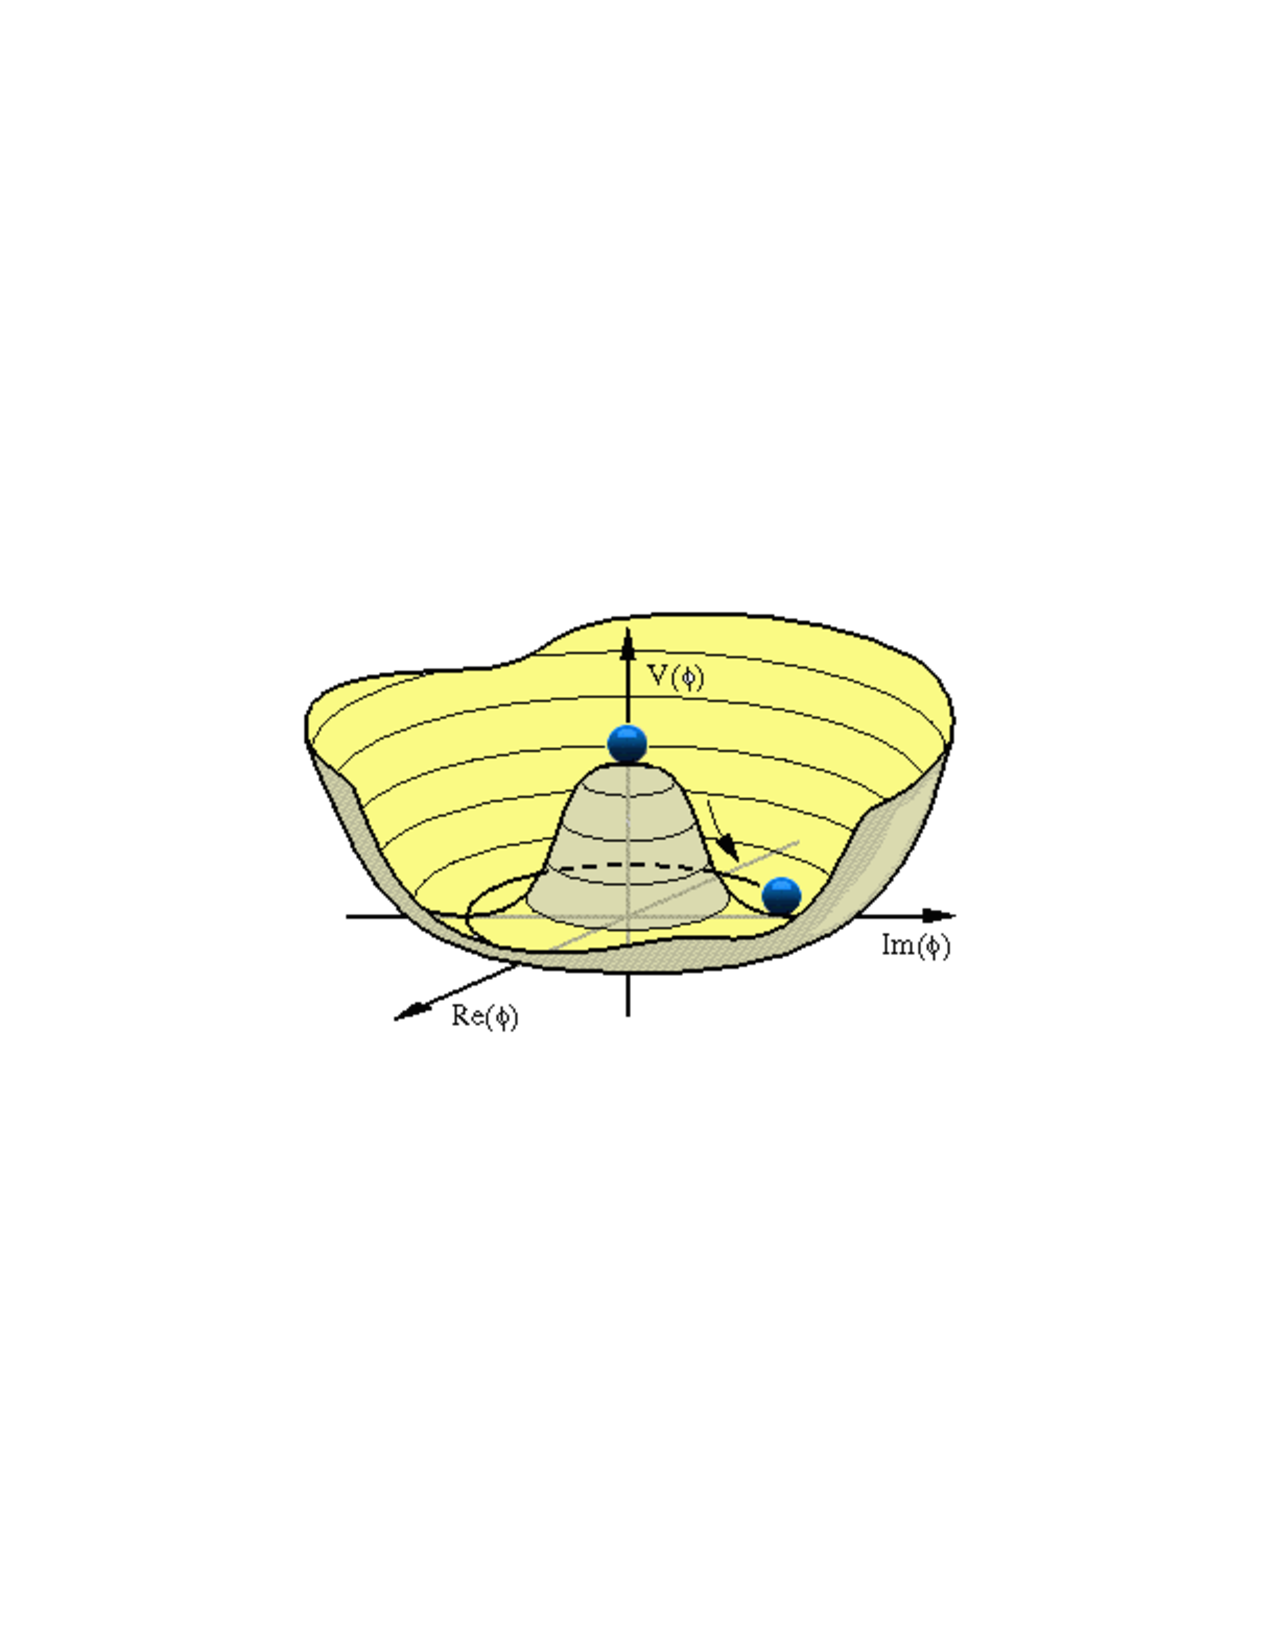
\includegraphics[width=0.5\textwidth]{Figures/Basic_Diagrams/higgs-potential.pdf}
  \caption{A visual representation of the Higgs potential} \label{fig:higgs_potential}
\end{figure}

\noindent if $\mu^{2}>0$ the shape of the potential no longer has a
mimium at $\langle\phi\rangle = 0$.  Figure \ref{fig:higgs_potential}
shows a plot of the potential energy of $\phi$ in terms of each of its
components.  The new minimum potential energy
occurs at:

\begin{equation}\label{eq:abelian_higgs_mechanism_potential_min}
\langle\phi\rangle = \phi_{0} = \left(\frac{\mu^{2}}{\lambda}\right)^{1/2}
\end{equation}

\noindent and while the field has a ground state at the zero potential
point it is in an unstable equilibrium.  Any quantum fluctuation about
this point will take the field into the lower energy configuration
with a ground state about the new minimum.  When the Langrangian is
expanded about~\ref{eq:abelian_higgs_mechanism_potential_min}, the
field, $\phi$ is rewritten as: 

\begin{equation}\label{eq:abelian_higgs_mechanism_expanded_phi}
\phi(x) = \phi_{0} + \frac{1}{\sqrt{2}}(\phi_{1}(x) + i\phi_{2}(x)
\end{equation}

\noindent the potential term, $V(x)$, then becomes:

\begin{equation}\label{eq:abelian_higgs_mechanism_expanded_pot}
V(x) = -\frac{1}{2\lambda}\mu^{4} +
\frac{1}{2}\cdot2\mu^{2}\phi_{1}^{2} + \mathcal{O}(\phi_{i}^{3})
\end{equation}

\noindent where we can notice that $\phi_{1}$ has acquired a mass term
with, $m = \sqrt{2}\mu$, while the scalar field $\phi_{2}$ remains
massless, and is known as the Goldstone boson.  The covariant
derivative is also tranformed as:

\begin{equation}\label{eq:abelian_higgs_mechanism_expanded_covDer}
|D_{\mu}\phi|^{2} = \frac{1}{2}(\partial_{\mu}\phi_{1})^{2} +
\frac{1}{2}(\partial_{\mu}\phi_{2})^{2} +
\sqrt{2}e\phi_{0}\cdot~A_{\mu}\partial^{\mu}\phi_{2} +
e^{2}\phi_{0}^{2}A_{\mu}A^{\mu} + ...
\end{equation}

\noindent where cubic and quartic terms of $A_{\mu}$, $\phi_{1}$,
and $\phi_{2}$ have been dropped.  The important term is the last one,
which can be interpreted as a mass term of the vector field, $A_{\mu}$

\begin{equation}\label{eq:abelian_higgs_mechanism_mass_term_Amu}
\Delta\mathcal{L}_{M} =
  \frac{1}{2}m_{A}A_{\mu}A^{\mu} = e^{2}\phi_{0}^{2}A_{\mu}A^{\mu}
\end{equation}

\noindent where $m_{A} = 2e^{2}\phi_{0}^{2}$, has arisen from
consequences of a non-zero vacuum expectation value of the $\phi$
field.  The remaining, massless Godlstone boson, $\phi_{2}$ is not a
physical particle, but rather a consequence of the choice of guage.
This is illustrated when we can use the $U(1)$ guage symmetry to rotate
the field $\phi(x)$ such that the field disapears.  

\begin{equation}\label{eq:abelian_higgs_mechanism_rotate_phi2}
\begin{aligned}
 \phi \rightarrow \phi' & = e^{i\alpha}(\phi_{1} + \phi_{2}) \\
& = (\cos{\alpha} + i\sin{\alpha})(\phi_{1} + \phi_{2}) \\
& = (\phi_{1}\cos{\alpha} - \phi_{2}\sin{\alpha}) +
i(\phi_{1}\sin{\alpha} + \phi_{2}\cos{\alpha}) \\
& = (\phi_{1} - \phi_{2}\tan{\alpha}) + i(\phi_{1}\tan{\alpha} +
\phi_{2})
\end{aligned}
\end{equation}

\noindent Choosing $\alpha = -\tan{\phi_{2}/\phi_{1}}$ will make $\phi'$
 a real quantity and elminate it's imaginary component, $\phi_{2}'$.
 The lagrangian can then be rewritten in terms of the rotated field
 $\phi'$ and see that massless boson is indeed removed from the
 theory.

\begin{equation}\label{eq:abelian_higgs_mechanism_final_lagrangian}
\begin{aligned}
\mathcal{L} & =
\frac{1}{2}(\partial_{\mu}\phi_{1}')(\partial^{\mu}\phi_{1}') -
\frac{1}{2}\cdot~2\mu^{2}\phi_{1}'\phi_{1}' \\
&  -\frac{1}{4}(F^{\mu\nu}F_{\mu\nu}) +
\frac{1}{2}\cdot~e^{2}\phi_{0}^{2}A_{\mu}A^{\nu} \\
&  + \phi_{0}e^{2}\phi_{1}'A_{\mu}A^{\mu} +
\frac{1}{2}e^2\phi_{1}'^{2}A_{\mu}A^{\mu} + \mathcal{O}(\phi'^{3})...
\end{aligned}
\end{equation}

\par The degree of freedom that $\phi_{2}$ represents, is absorbed as
a longitudanal polarization of the $A_{mu}$ field, a forbidden for
massless guage bosons, but necessary for massive bosons.  

\par For this case of an abelian symmetry $U(1)$, it was shown that if a
complex scalar field, which interacts with itself and another vector
field, can gains a non-zero vacuum expectation value.  The Lagrangian can
be expanded about this new mimimum, generating a mass term for the
vector field.  One of the degrees of freedom of the orginial complex
scalar field is then absorbed as a longitudanal polarization state of
the massive vector field.  

\section{The Higgs Mechanism in a non-Abelian Theory}
\label{non_abelian_higgs_mechanism_overview}

\par Before describing the elctroweak guage theory of
$SU(2)\otimes~U(1)$, it will be helpful to see the effects of the
Higgs mechanism for the non-Abelian group, $SU(2)$ by itself.  Consider an
an example of an $SU(2)$ gauge field coupled to a scalar field that
transforms like a real-valued vector under $SU(2)$
transformations~\cite{Peskin_Schroeder}.  The field $\phi$ will have
the form:

\begin{equation}\label{eq:non_abelian_higgs_mechanism_phi}
\phi = 
  \begin{pmatrix}
    \phi_{1} \\
    \phi_{2} \\
    \phi_{3}
    \end{pmatrix}
\end{equation}

\noindent where the components, $\phi_{i}$ are real-valued fields.
The $SU(2)$ transformation for this scalar field will also look like:

\begin{equation}\label{eq:non_abelian_higgs_mechanism_transformation}
\phi \rightarrow e^{i\alpha^{i}T^{i}}\phi
\end{equation}

\noindent where the matrices, $T^{i}$ are defined as:

\tiny
\begin{equation}\label{eq:non_abelian_higgs_mechanism_generators}
iT^{1} = 
  \begin{pmatrix}
    0  &  0  &  0 \\
    0  &  0  &  1 \\
    0  & -1 &  0 
  \end{pmatrix}
\text{   ,    }
T^{2} = 
  \begin{pmatrix}
    0  &  0  & -1 \\
    0  &  0  &  0 \\
    1  &  0  &  0 \\ 
  \end{pmatrix}
\text{   ,   }
T^{3} = 
  \begin{pmatrix}
    0  &   1  &  0 \\
   -1 &   0  &  0 \\
    0  &   0  &  0
  \end{pmatrix}
\end{equation}
\normalsize

\noindent The Lagrangian for this field will feature a Higgs potential
term along with the previously mentioned $SU(2)$ guage fields, $A_{\mu}^{a}$ coupled
to the scalar field, $phi$, and is given by:

\begin{equation}\label{eq:non_abelian_higgs_mechanism_lagrangian}
\mathcal{L} = -\frac{1}{4}F_{\mu\nu}^{a}F^{a\mu\nu}+ |D_{\mu}\phi|^{2}
+ \mu^{2}\phi^{\ast}\phi - \frac{\lambda}{4}(\phi^{\ast}\phi)^{2}
\end{equation}

\noindent where $F_{\mu}{\nu}^{a}$, the field strength tensor is
defined as:

\begin{equation}\label{eq:non_abelian_higgs_mechanism_field_strength_tensor}
F_{\mu\nu}^{a} = (\partial_{\mu}A_{\nu}^{a}
- \partial_{\nu}A_{\mu}^{a}) + g\epsilon^{abc}A_{\mu}^{b}A_{\nu}^{c}
\end{equation}

\noindent and the covariant derivative is defined as:

\begin{equation}\label{eq:non_abelian_higgs_mechanism_covariant_derivative}
D_{\mu} = (\partial_{\mu} + igA_{\mu}^{a}T^{a})\phi
\end{equation}

\par Similarly to the Abelian case, the Higgs potential will induce a
spontaneous symmetry breaking, and one of the components of the field
$\phi$ will gain a vacuum expectation value.  After this breaking and
expanding around the ground state potential, the
field $\phi$ will have the form:

\begin{equation}\label{eq:non_abelian_higgs_mechanism_phi_broken}
\phi = \frac{1}{\sqrt{2}}
  \begin{pmatrix}
    0 \\
    0 \\
    v + h
    \end{pmatrix}
\end{equation}

\noindent There has been no loss in generality in assuming this form
since, similarly to the abelian case, we can use the gauge symmetry of
$SU(2)$ to rotate the field into this configuration.  Goldstone's
theorem tells us that we should expect two massive gague bosons
corresponding to the $T^{1}$, and $T^{2}$ generators, while the
$T^{3}$ generator will correspond to a massless gauge boson, since
$\phi$ is still invariant under $T^{3}$ transformations. 

\par As in the Abelian case, the mass terms for the gauge bosons are
generated from the covariant derivative term, $|D_{\mu}\phi|^{2}$

\begin{equation}\label{eq:non_abelian_higgs_mechanism_covariant_derivative_on_phi}
\begin{aligned}
D_{\mu}\phi & = \frac{1}{\sqrt{2}}\left(~\partial_{\mu} + gA_{\mu}^{1}
  \begin{pmatrix}
    0  &  0  &  0 \\
    0  &  0  &  1 \\
    0  & -1 &  0 
  \end{pmatrix}
  + gA_{\mu}^{2}
  \begin{pmatrix}
    0  &  0  & -1 \\
    0  &  0  &  0 \\
    1  &  0  &  0 \\ 
  \end{pmatrix}
+ gA_{\mu}^{3}
  \begin{pmatrix}
    0  &   1  &  0 \\
   -1 &   0  &  0 \\
    0  &   0  &  0
  \end{pmatrix}
\right)
  \begin{pmatrix}
    0 \\
    0 \\
    v + h
  \end{pmatrix} \\
 & = \frac{1}{\sqrt{2}}
  \begin{pmatrix}
    0 \\
    0 \\
    \partial_{\mu}
  \end{pmatrix}
  + \frac{gA_{\mu}^{1}}{\sqrt{2}}
  \begin{pmatrix}
    0 \\
    v+h \\
    0
  \end{pmatrix}
  - \frac{gA_{\mu}^{2}}{\sqrt{2}}
  \begin{pmatrix}
    v+h \\
    0 \\
    0
    \end{pmatrix} \\
 & = \frac{1}{\sqrt{2}}
  \begin{pmatrix}
    g(v+h)A_{\mu}^{1} \\
    g(v+h)A_{\mu}^{2} \\
    \partial_{\mu}h
  \end{pmatrix}
\end{aligned}
\end{equation}

\noindent Therefore

\begin{equation}\label{eq:non_abelian_higgs_mechanism_covariant_derivative_sq}
|D_{\mu}\phi|^{2} = \frac{1}{2}\partial_{\mu}h\partial^{\mu}h +
\frac{g^{2}v^{2}}{2}\left( (A_{\mu}^{1})^{2} + (A_{\mu}^{2})^{2} \right) +
\frac{g^{2}}{2}(h^{2}+2hv)\left( (A_{\mu}^{1})^{2} + (A_{\mu}^{2})^{2} \right)
\end{equation}

\par This theory produces two massive bosons, $A_{\mu}^{1}$ and
$A_{\mu}^{2}$, both with mass, $m_{A} = gv$.  These fields have $h$,
and $h^2$ couplings to the Higgs boson.  The third guage field,
$A_{\mu}^{3}$, remains massles and is not coupled to the Higgs field.
This model is beginning to resemble a description of electroweak
physics, however, a third massive boson is necessary, as is a new
gague symmetry in order to generate it.  That is the subject of the
next section.  

\section{Glashow Weinberg Salam Theory}
\label{ewk_overview}

\par Glashow, Weinberg, and Salam published their theory unifying
elctromagnetic and weak forces in the
1960s~\cite{th:Weinberg_ModelOfLeptons}~\cite{th:Glashow_PartialSymmetries}~\cite{th:Salam_EWKInteractions}.
It begins with the requirement of a $SU(2)_{L}\otimes~U(1)$
symmetry and incorporates the Higgs mechanism to give mass to the guage bosons
of the weak force.  As described earlier, the $U(1)$ symmetry requires
introducing a vector field, which will be labeled $B_{\mu}$, and an interaction term, which
is absorbed into the covariant derivative, $D_{\mu}$.  The
transformation will also be paramaterized with a with a quantum
number, $Y$, known as hypercharge.  The $SU(2)$
symmetry requires the introduction of three new 
vector fields, which will be labeled $W_{\mu}^{i}, i = 1, 2, 3$.  The
quantum number associated with this gauge group is known as isospin,
and is determined by the $T^{3}$ operator, acting on an $SU(2)$
doublet on the third generator of the group. The $SU(2)\otimes~U(1)$
transformation, $U(x)$, will then be give by:   

\begin{equation}\label{eq:ewk_su2_su1_transformation}
U(x) = e^{i\alpha^{a}(x)\tau^{a}}e^{iY\alpha(x)/}
\end{equation}

\noindent where $\tau^{a} = \sigma^{a}/2$, the Pauli matrices,
\ref{eq:pauli_matrices}.  These gauge fields will be coupled, via the
covariant derivative, to a doublet of complex scalar fields $\phi$,
with hypercharge $Y=+1/2$.  A Higgs potential will be added to 
generate the spontaneous symmetry breaking that will give mass to
three of the guage fields, and leave one massless.  In order to
preserve the $SU(2)_{L}\otimes~U(1)$ symmetry, the new covariant 
derivative will take the form:

\begin{equation}\label{eq:ewk_covariant_derivative}
D_{\mu} = (\partial_{\mu} - igW_{\mu}^{a}\tau^{a} -
\frac{i}{2}g'B_{\mu})
\end{equation}

\par The subscript L on $SU(2)_{L}$ refers to the experimental
results that the weak force violates parity maximally, by only
interacting with the left-handed chiral component of a field.  Right
versus left chiralty is determined by whether the spin of a particle
is aligned or anti-aligned with its direction of motion, and in
general a particle is represented by a linear combination of its right and
left handed components.  This idea was first proposed by Chen Ning
Yang and Tsung-Dao Lee, in the 1950s.  Their ideas were validated by
the experimental discovery of partiy violation in 1957, through the beta decays of Cobalt
60 atoms by C.S Wu.  That same year, Yang and Lee were awrded the
nobel prize for their insight~\cite{th:YangLee_NobelPrize}.  In this
model, then, the left-handed components of the particles participate
in the weak interaction and are formed into doublets, while the right handed
components are singlets, and will only interact with the
electromagnetic field, $B_{\mu}$.  The quantum numbers of the doublet
will be given by +1/2 for the upper component of the $SU(2)$ doublet,
and -1/2 for the lower component.  The fermion content of this theory
is then given by:

\begin{equation}\label{eq:ewk_fermion_doublets}
\begin{aligned}
&\binom{\nu_{L}}{e_{L}}, e_{R} \\
&\binom{u_{L}}{d_{L}}, u_{R}, d_{R} 
\end{aligned}
\end{equation}

\noindent where the right handed neutrino, $\nu_{R}$ has been ommited,
since it has zero charge, and isospin, and therefore does not
participate in any of the interactions of this theory.  The complete
Lagrangian is given by a sum of free particle terms for  massless bosons,
fermions, and Higgs scalar fields; the Higgs potential; and a Yukawa
coupling term between the fermions and the Higgs, which generates
their masses. 

\begin{equation}\label{eq:ewk_lagrangian_simple}
\mathcal{L}_{GWS} = \mathcal{L}_{Boson KE} + \mathcal{L}_{Higgs} +
\mathcal{L}_{Fermion KE} + \mathcal{L}_{Yukawa} 
\end{equation}

\noindent The Higgs potential will have the form:
\begin{equation}\label{eq:ewk_higgs_lagrangian_term}
\mathcal{L}_{Higgs} = (D_{\mu}\phi)^{\dagger}(D^{\mu}\phi)
+\mu^{2}\phi^{\dagger}\phi - \lambda(\phi^{\dagger}\phi)^{2}
\end{equation}

\noindent The Higgs potential will break the symmetry of
the Lagrangian when one of the four degrees of freedom in the
complex scalar doublet, $\phi$, spontaneously acquires a
vacuum expectation value.  In this case, it will generate
three massive gauge bosons, one massless gauge boson, and a massive
scalar field.  After gaining a vacuum expectation value, and expanding
about this value, the scalar fields will have the form:

\begin{equation}\label{eq:ewk_phi_vev}
\langle\phi\rangle = \frac{1}{\sqrt{2}}\binom{0}{v+h}
\end{equation}

\noindent where no loss of generality has occured since we are always
able to rotate into this form through the appropriate gauge
transformations, similar to what was descibed in the Abelian case.  It
should also be noted that this form is not invariant to any of the
individual generators $t^{a}$, however $\phi$ will be invariant to a
combination of $T^{3}+Y$ generators.  Per Goldstone's thereom, we
should expect this linear combination of fields to be the massless
vector boson after symemtry breaking.  The massless eigenstate will be
the electromagnetic field, $A_{\mu} \sim~A_{\mu}^{3} + B_{\mu}$.  The
electric charge quantum number, $Q$, is then defined as 
\begin{equation}\label{ewk_Q_quantum_number}
Q = T^{3}+Y
\end{equation}

\par As before, the generation of the masses for the guage bosons are
generated by the interaction of their fields with the Higgs field via
the covariant derivative.  

\begin{equation}\label{eq:ewk_covariant_derivative_acting_on_phi}
\begin{aligned}
D_{\mu}\phi & = \frac{1}{\sqrt{2}}\left( \partial_{\mu}
  - \frac{ig}{2}A_{\mu}^{1} 
  \begin{pmatrix}
    0  &  1 \\
    1  &  0
  \end{pmatrix}
  - \frac{ig}{2}A_{\mu}^{2} 
  \begin{pmatrix}
    0  & -i \\
    i  &  0
  \end{pmatrix}
  - \frac{ig}{2}A_{\mu}^{3} 
  \begin{pmatrix}
    1  &   0 \\
    0  & -1
  \end{pmatrix}
\right)\binom{0}{v+h} \\ \\
& = \frac{1}{\sqrt{2}}\binom{(\frac{g}{2}(v+h)A_{\mu}^{2}) +
  i(\frac{g}{2}(v+h)A_{\mu}^{1})}{\partial_{\mu} +
  i(\frac{1}{2}(v+h)(gA_{\mu}^{3}-g'B_{\mu}))}
\end{aligned}
\end{equation}

\noindent Taking the dot product of this with its hermitian conjugate
gives the $|D_{\mu}\phi|^{2}$ term:

\begin{equation}\label{eq:ewk_partial_phi_squared}
\begin{aligned}
|D_{\mu}\phi|^{2} = & \frac{1}{2}\partial_{\mu}h\partial^{\mu}h +
\frac{1}{2}\frac{g^{2}v^{2}}{4}( (A_{\mu}^{1})^{2} + (A_{\mu}^{2})^{2}
) +\frac{v^{2}}{4}(gA_{\mu}^{3}-g'B_{\mu})^{2}  \\
 & + \frac{1}{2}{g^{2}}{4}(h^{2}+2vh)( (A_{\mu}^{1})^{2} +
 (A_{\mu}^{2})^{2} ) +
 \frac{1}{2}\frac{1}{4}(h^{2}+2vh)(gA_{\mu}^{3}-g'B_{\mu}) 
\end{aligned}
\end{equation}

\noindent From equation~\ref{eq:ewk_partial_phi_squared} we
can identify three massive and one massless guage bosons,
corresponding the the charged and nuetral weak currents, and the
elctromagnetic current.  

\begin{equation}\label{eq:ewk_boson_masses}
\begin{aligned}
W_{\mu}^{\pm} & = \frac{1}{\sqrt{2}}(A_{\mu}^{1} \mp iA_{\mu}^{2}) 
&\text{  with mass  }  m_{W} &= g\frac{v}{2}\text{;} \\
Z_{\mu}^{0} & = \frac{1}{\sqrt{g^{2}+g'^{2}}}(gW_{\mu}^{3}-g'B_{\mu})  
&\text{  with mass  }  m_{Z} &= \frac{v}{2}\sqrt{g^{2}+g'^{2}}\text{;}  \\
A_{\mu} & = \frac{1}{\sqrt{g^{2}+g'^{2}}}(gW_{\mu}^{3}+g'B_{\mu}) 
&\text{  with mass  }  m_{A} &= 0 \text{;} 
\end{aligned}
\end{equation}

\noindent where the last field, $A_{\mu}$ is absent from the covariant
derivative term, but already identified as the massless gauge boson of
the theory due to it's gauge invariance under a $T^{3}+Y$ rotation.
Using these definitions the covariant derivative has the following
form:

\begin{equation}\label{eq:ewk_covariant_derivative_mass_eigenstates}
\begin{aligned}
D_{\mu} & = \partial_{\mu} - \frac{ig}{\sqrt{2}}(W^{+}T^{+} + W^{-}T^{-}) \\
  &  - \frac{i}{\sqrt{g^{2}+g'^{2}}}Z_{\mu}^{0}(gT^{3} - g'Y) -
    \frac{gg'}{\sqrt{g^{2}+g'^{2}}}A_{\mu}(T^{3}+Y) 
\end{aligned}
\end{equation} 

\noindent where $T^{\pm} = \frac{1}{2}(\sigma^{1}\pm\sigma^{2})$.  From
this form, we can identiy the fundamental electric charge, $e$, as

\begin{equation}\label{eq:ewk_electric_charge}
e = \frac{gg'}{\sqrt{g^{2}+g'^{2}}}
\end{equation}

The similarity in the forms between $Z_{\mu}^{0}$ and $A_{\mu}$
suggest that their relationship can be expressed in a simpler form, as
the rotation of underlying guage fields $A_{\mu}^{3}$ and $B_{\mu}$
through the weak mixing angle, $\theta_{W}$

\begin{equation}\label{eq:weak_mixing_matrix}
\binom{Z_{\mu}^{0}}{A_{\mu}} = 
\begin{pmatrix}
    \cos{\theta_{W}} & -\sin{\theta_{W}} \\
    \sin{\theta_{W}}  &  \cos{\theta_{W}}
  \end{pmatrix}
\binom{A_{\mu}^{3}}{B_{\mu}}
\end{equation}

\noindent where $\tan{\theta_{W}} = \frac{g'}{g}$.  Expanding
\ref{eq:weak_mixing_matrix}, we have the definitions of the
$Z_{\mu}^{0}$ and $A_{\mu}$ fields in terms of $\theta_{W}$

\begin{equation}\label{eq:ewk_Z_A_defined_with_thetaW}
\begin{aligned}
Z_{\mu}^{0} &= A_{\mu}^{3}\cos{\theta_{W}} - B_{\mu}\sin{\theta_{W}}
\\
A_{\mu} & = A_{\mu}^{3}\sin{\theta_{W}} + B_{\mu}\cos{\theta_{W}}
\end{aligned}
\end{equation}

\noindent The weak mixing angle, $\theta_{W}$, also provides a
simple relationship between the $W_{\mu}^{\pm}$ and $Z_{\mu}^{0}$
fields:

\begin{equation}\label{eq:ewk_mz_is_mwcosthetaW}
m_{W} = m_{Z}\cos{\theta_{W}}
\end{equation}

\noindent The covariant derivative, $D_{\mu}$ is also rewritten in
terms of the mass eignenstates of the gauge fields

\begin{equation}\label{eq:ewk_covariant_derivative_mass_eigenstates}
D_{\mu} = (\partial_{\mu} - \frac{ig}{\sqrt{2}}(W_{\mu}^{+} +
W_{\mu}^{-}T^{-}) -
\frac{ig}{\cos{\theta_{W}}}Z_{\mu}^{0}(T_{3}-sin^{2}{\theta_{W}}Q) -
ieA_{\mu}Q)
\end{equation}

\noindent where $g = e/\cos{\theta_{W}}$.  The square of the covariant
derivative is then written as

\begin{equation}\label{eq:ewk_covariant_derivative_squared_mass_eigenstates}
\begin{aligned}
|D_{\mu}|^{2} &= \frac{1}{2}\partial_{\mu}h\partial^{\mu}h +
\frac{1}{2}m_{W}^{2}W_{\mu}^{+}W^{\mu+} +
\frac{1}{2}m_{W}^{2}W_{\mu}^{-}W^{\mu-} +
\frac{1}{2}m_{Z}^{2}Z_{\mu}^{0}Z^{\mu0} \\
& + (\frac{h^{2}}{v^{2}} + \frac{h}{v})[
    \frac{1}{2}m_{W}^{2}(W_{\mu}^{+}W^{\mu+}+W_{\mu}^{-}W^{\mu-}) +
    \frac{1}{2}m_{Z}^{2}Z_{\mu}^{0}Z^{\mu0}]
\end{aligned}
\end{equation} 
\\
\par With the form of the covariant derivative in place, the
fermionic kinematic term of the Lagrangian can be described.  As
mentioned earlier, the masses of the fermions in the model will be
generated by the Yukawa interaction term with the Higgs, so this
term only involves the covariant derivatives acting on the left-handed
doublet and right-handed singlet states of this model.  

\begin{table}[h]
  \begin{center}
%                              vl  el  er  ul  dl  ur  dr
  \begin{tabular}{ | l | c | c | c | c | c | c | c | } \hline
    & $\nu_{L}$ & $e_{L}$ & $e_{R}$ & $u_{L}$ & $d_{L}$ & $u_{R}$ &
    $d_{R}$ \\ \hline
    Isospin & +1/2 & -1/2 & 0 & +1/2 & -1/2 & 0 & 0 \\ \hline
    Hypercharge & -1/2 & -1/2 & -1 & +1/6 & 1/3 & 2/3 & -1/3 \\ \hline
    Electric Charge & 0 & -1 & -1 & 2/3 & -1/3 & 2/3 & -1/3 \\ \hline
  \end{tabular}
  \caption{ The quantum numbers Isospin and Hypercharge are assigned for each of the $SU(2)$ and
      $U(1)$ symmetries respectively}
    \label{tab:ewk_fermion_quantum_numbers}
  \end{center}
\end{table} 

\noindent The quantum number assignments for the leptons, which are
chosen in order to reproduce the known values of their electric
charges, are shown in table~\ref{tab:ewk_fermion_quantum_numbers}.
The values  of these quantum numbers enter into the covariant
derivative via the  $Z_{\mu}^{0}$ term of equation
\ref{eq:ewk_covariant_derivative_mass_eigenstates}.  The fermionic
kinetic energy term of the Lagrangian is given by:

\begin{equation}\label{eq:ewk_fermionic_lagrangian_term}
\begin{aligned}
\mathcal{L}_{Fermion} =&~ \bar{E}_{L}(i\gamma^{u}D_{\mu})E_{L} +
\bar{e}_{R}(i\gamma^{u}D_{\mu})e_{R} \\
&~ \bar{Q}_{L}(i\gamma^{u}D_{\mu})Q_{L} +
\bar{u}_{R}(i\gamma^{u}D_{\mu})u_{R} +
\bar{d}_{R}(i\gamma^{u}D_{\mu})d_{R}
\end{aligned}
\end{equation} 

\noindent Expanding the covariant term for the left-handed electron
shows its explicit coupling to the guage boson fields. 

\begin{equation}\label{eq:ewk_eLeft_lagrangian_term}
\begin{aligned}
\mathcal{L}_{E_{L}} =&~ 
\begin{pmatrix}
  \bar{\nu_{L}} & \bar{e_{L}} 
\end{pmatrix}
\left( (i\gamma^{\mu}(\partial_{\mu} -
  \frac{ig}{\sqrt{2}}(W_{\mu}^{+}T^{+} + W_{\mu}^{-}T^{-}) -
  \frac{ig}{\cos{\theta_{W}}}Z_{\mu}^{0}(T^{3}-\sin^{2}{\theta_{W}}Q)
  - ieA_{\mu}Q)~)~\right)\binom{\nu_{L}}{e_{L}} \\
=&~\bar{\nu_{L}}i\gamma^{\mu}\partial_{\mu}\nu_{L} +
\bar{e_{L}}i\gamma^{\mu}\partial_{\mu}e_{L}
+\frac{ig}{\sqrt{2}}W_{\mu}^{+}\bar{\nu_{L}}\gamma^{\mu}e +
\frac{ig}{\sqrt{2}}W_{\mu}^{-}\bar{e_{L}}\gamma^{\mu}\nu_{L} \\
&~+\frac{ig}{\cos{\theta_{W}}}\bar{\nu_{L}}(1/2)\gamma^{\mu}\nu_{L} +
\frac{ig}{\cos{\theta_{W}}}\bar{e_{L}}\gamma^{\mu}(-1/2 +
\sin^{2}{\theta_{W}}(+1))e_{L} + (ie)\bar{e_{L}}\gamma^{\mu}A_{\mu}(-1)
\end{aligned}
\end{equation}

\noindent All of the terms will be combined with the final,
spontaneously broken GWS Lagranian at the end of this section.  

\par The final term to discuss in the theory, before combing all of
the results, is the Yukawa interaction term between the fermion fields
and the Higgs.  For the electron, this term takes the form:

\begin{equation}\label{eq:ewk_yukawa}
\begin{aligned}
\mathcal{L}_{Yukawa} =&~ -\lambda_{e}\bar{E_{L}}\cdot\phi~e_{R} -
\lambda_{e}E_{L}\cdot\phi~\bar{e_{R}} \\
=&~ -\frac{\lambda_{e}}{\sqrt{2}}(v+h)(\bar{e_{L}}e_{R} +
  e_{L}\bar{e_{R}}) \\
=&~ --\frac{\lambda_{e}v}{\sqrt{2}}(\bar{e_{L}}e_{R} +
  e_{L}\bar{e_{R}}) + -\frac{\lambda_{e}}{\sqrt{2}}(\bar{e_{L}}e_{R} +
  e_{L}\bar{e_{R}})h
\end{aligned}
\end{equation}

\noindent where the mass of the electron is identified as $m_{e} =
\frac{\lambda_{e}v}{\sqrt{2}}$.  In order to generate the masses of
the particles, each fermion has its own unique $\lambda$ value.  So
while the Higgs mechanism is able to generate the masses in a way that
preserves the underlying $SU(2)\otimes~U(1)$ symmetry, it does not
explain the heirarchy of masses since each $\lambda$ value is unique
to each lepton.  The second term in last equation of
~\ref{eq:ewk_yukawa} is the coupling of the Higgs particle, $h$, to
the fermions.  The coupling is proportional to the mass of the
particle.  The largest of these is to the top quark, with $m_{t} =
73.21 \pm 0.51 \pm 0.71 GeV$.

\par The Yuakawa coupling for the quarks is necessarily modified when
additional quarks besides the $u$ and $d$ are added to the theory.
This is because there can be additional coupling terms that mix
generations.  This occurs when the mass eigenstate of the quarks is
not the same as the interaction eigenstate.  The modification requires
the expansion of the $u_{L}$ and $d_{L}$ components into a vector of
left handed quarks.  If we let

\begin{equation}\label{eq:ewk_quark_vector}
\begin{aligned}
u_{L}^{i} = (u_{L}, c_{L}, t_{L}) &,                 & d_{L}^{i} = (d_{L}, s_{L}, b_{L})
\end{aligned}
\end{equation}

\noindent represent the up and down-type quarks in the orginal weak
interaction basis, then the vectors, $u_{L}^{i}$' and $d_{L}^{i}$',
can be defined as the diagonlized basis for the Higgs coupling.  They
are related through a unitary transformation.  

\begin{equation}\label{eq:ewk_quark_transformaitons}
\begin{aligned}
u_{L}^{i} = U_{u}^{ij}u_{L}^{j\prime} &,                 & d_{L}^{i} = U_{d}^{ij}d_{L}^{j\prime}
\end{aligned}
\end{equation}

\noindent The interaction terms with the charged gauge boson currents
must then be rewritten as

\begin{equation}\label{eq:ewk_ckm_intro}
J_{W}^{\mu+} = \frac{1}{\sqrt{2}}\bar{u_{L}^{i}}\gamma^{\mu}d_{L}^{i}
=
\frac{1}{\sqrt{2}}\bar{u_{L}^{i\prime}}\gamma^{\mu}(U_{u}^{\dagger}U_{d})d_{L}^{j\prime}
= \frac{1}{\sqrt{2}}\bar{u_{L}^{i\prime}}\gamma^{\mu}V_{ij}d_{L}^{j\prime}
\end{equation}

\noindent where $V_{ij}$ is the 3x3 Cobibbo-Kobayashi-Maskawa (CKM) matrix
describing the mixing among six
quarks~\cite{th:CKM_matrix_C}~\cite{th:CKM_matrix_KM}.  It is an
extension of the Glashow-Iliopoulos-Maiaini mechanism, which was a 2x2
matrix that predicted the existence of a fourth quark, the charm quark.  The GIM
mechanism was an attempt to suppress flavor-changing-neutral currents,
which occur at LO in a three-quark model, but not in a four-quark
model.  The CKM matrix, however, was motivated by an attempt to
explain $CP$ violation in the weak interaction.  At the time of its
publication, the bottom and top quarks were not predicted.  After
these were discovered, they were awarded the nobel prize in physics in
2008.  

\par At this point, all the of the pieces are ready to write down the
GWS Lagrangian, after the Higgs mechanism has spontaneously broken the
$SU(2)\otimes~U(1)$ symmetry.

\begin{equation}\label{eq:ewk_lagrangian_unbroken}
\begin{aligned}
\mathcal{L}_{Unbroken} = &~ -\frac{1}{4}A_{\mu\nu}^{a}A^{\mu\nu~a} -
\frac{1}{4}F_{\mu\nu}F^{\mu\nu} \\
&~ + |D_{\mu}\phi|^{2} + \mu^{2}(\phi^{\dagger}\phi) - \lambda(\phi^{\dagger}\phi)^{2} \\
&~ + \bar{E_{L}}(i\gamma^{\mu}D_{\mu})E_{L} + \text{ similar terms for }
    e_{R}, U_{L}, u_{R}, d_{R} \\
&~ -\lambda_{e}\bar{E_{L}}\cdot\phi~e_{R} + h.c. + \text{ similar
  terms for } e_{R}, U_{L}, u_{R}, d_{R}
\end{aligned}
\end{equation}

\begin{equation}\label{eq:ewk_lagrangian_broken}
\begin{aligned}
\mathcal{L}_{GWS} = &~ -\frac{1}{4}(Z_{\mu\nu}^{0})^{2} -
\frac{1}{2}(W_{\mu\nu}^{+}W_{\mu\nu}^{-}) -
\frac{1}{4}(F_{\mu\nu})^{2}  \\
&~ + ig\cos{\theta_{W}}\left( (W_{\mu}^{-}W_{\nu}^{+} -
  W_{\nu}^{-}W_{\mu})\partial^{\mu}Z^{0\nu} +
  W_{\mu\nu}^{+}W^{-\mu}Z^{0\nu} + W_{\mu\nu}^{-}W^{+\mu}Z^{0\nu}
\right) \\ 
&~ + ie\left(
  (W_{\mu}^{-}W_{\nu}^{+}-W_{\nu}^{-}W_{\mu}^{+})\partial^{\mu}A^{\nu}
  + W_{\mu\nu}^{+}W^{-\mu}A^{\nu} - W_{\mu\nu}^{-}W^{+\mu}A^{\nu}
\right)\\
&~ + g^{2}\cos^{2}{\theta_{W}}\left(
  W_{\mu}^{+}W_{\nu}^{-}Z^{0\mu}Z^{0\nu} -
  W_{\mu}^{+}W^{-\mu}Z_{\nu}^{0}Z^{0\nu} \right) \\
&~ + g^{2}\left( W_{\mu}^{+}W_{\mu}^{-}A^{\mu}A^{\nu} -
  W_{\mu}^{+}W^{-\mu}A_{\nu}A^{\nu} \right) \\
&~ + ge\cos{\theta_{W}}\left( W_{\mu}^{+}W_{\nu}^{-}(Z^{0\mu}A_{\nu} +
  Z^{0\nu}A^{\mu}) - 2W_{\mu}^{+}W^{-\mu}A^{\nu} \right) \\
&~ + \frac{1}{2}g^{2}(W_{\mu}^{+}W_{\nu}^{-})(W^{+\mu}W^{-\nu} -
W^{+\nu}W^{-\mu}) \\
&~ + \frac{1}{2}\partial_{\mu}h\partial^{\nu}h - v^{2}{\lambda}h^{2} +
\frac{1}{2}m_{W}^{2}W_{\mu}^{+}W^{+\mu} +
\frac{1}{2}m_{W}^{2}W_{\mu}^{-}W^{-\mu} +
\frac{1}{2}m_{Z}^{2}Z_{\mu}^{0}Z^{0\mu} \\
&~ + (\frac{h^{2}}{v^{2}} + \frac{h}{v})\left(
  \frac{1}{2}m_{W}^{2}(W_{\mu}^{+}W^{+\mu} + W_{\mu}^{-}W^{-\mu}) +
  \frac{1}{2}m_{Z}^{2}Z_{\mu}^{0}Z^{0\mu} \right) - {\lambda}vh^{3} - \frac{1}{4}{\lambda}h^{4} \\
&~ + \bar{E_{L}}(i\gamma^{\mu}\partial_{\mu})E_{L} +
\bar{e_{R}}(i\gamma^{\mu}\partial_{\mu})e_{R} +
\bar{Q_{L}}(i\gamma^{\mu}\partial_{\mu})Q_{L} +
\bar{u_{R}}(i\gamma^{\mu}\partial_{\mu})u_{R}  +
\bar{d_{R}}(i\gamma^{\mu}\partial_{\mu})d_{R} \\ 
&~ + g(W_{\mu}^{+}J_{W}^{\mu+} + W_{\mu}^{-}J_{W}^{\mu-} +
Z_{\mu}^{0}J_{Z}^{\mu}) + eA_{\mu}J_{EM}^{\mu} \\
&~ -\frac{\lambda_{e}v}{\sqrt{2}}(\bar{e_{L}}e_{R}+\bar{e_{R}}e_{L}) +
-\frac{\lambda_{e}h}{\sqrt{2}}(\bar{e_{L}}e_{R}+\bar{e_{R}}e_{L}) \\
&~ -\frac{\lambda_{u}v}{\sqrt{2}}(\bar{u_{L}}u_{R}+\bar{u_{R}}u_{L}) +
-\frac{\lambda_{u}h}{\sqrt{2}}(\bar{u_{L}}u_{R}+\bar{u_{R}}u_{L})  \\
&~ -\frac{\lambda_{d}v}{\sqrt{2}}(\bar{d_{L}}d_{R}+\bar{d_{R}}d_{L}) +
-\frac{\lambda_{d}h}{\sqrt{2}}(\bar{d_{L}}d_{R}+\bar{d_{R}}d_{L})  \\
\end{aligned}
\end{equation}

\noindent where the currents of the electroweak interaction,
$J_{W}^{\mu+}$, $J_{W}^{\mu-}$, $J_{Z}^{\mu}$, $J_{A}^{\mu}$ are
defined as:
\begin{equation}\label{eq:ewk_currents}
\begin{aligned}
J_{W}^{\mu+} =&~ \frac{1}{\sqrt{2}}\left(
  \bar{\nu_{L}}\gamma^{\mu}e_{L} + \bar{u_{L}^{i\prime}}\gamma^{\mu}V_{ij}d_{L}^{j\prime}
\right) \\ 
J_{W}^{\mu-} =&~ \frac{1}{\sqrt{2}}\left(
  \bar{e_{L}}\gamma^{\mu}\nu_{L} +
    \bar{d_{L}^{i\prime}}\gamma^{\mu}V_{ij}u_{L}^{j\prime} \right) \\
J_{Z}^{\mu} =&~ \frac{1}{\cos{\theta_{W}}}(
  \bar{\nu_{L}}\gamma^{\mu}(+1/2)\nu_{L} +
  \bar{e_{L}}\gamma^{\mu}(-1/2+\sin^{2}{\theta_{W}})e_{L} +
  \bar{e_{R}}\gamma^{\mu}\sin^{2}{\theta_{W}}e_{R} \\
&~ + \bar{u_{L}}\gamma^{\mu}(1/2-2/3sin^{2}{\theta_{W}})u_{L} +
\bar{u_{R}}\gamma^{\mu}(-2/3sin^{2}{\theta_{W}})u_{R} \\
&~ + \bar{d_{L}}\gamma^{mu}(-1/2+1/3sin^{2}{\theta_{W}})d_{L} +
\bar{d_{R}}\gamma^{\mu}(1/3sin^{2}{\theta_{W}})d_{R} ) \\
J_{EM}^{\mu} =&~ \bar{e_{L,R}}\gamma^{\mu}(-1)e_{L,R} +
\bar{u_{L,R}}\gamma^{\mu}(2/3)u_{L,R} + \bar{d_{L,R}}\gamma^{\mu}(-2/3)d_{L,R}
\end{aligned}
\end{equation}



\section{The Standard Model of Particle Physics}
\label{standard_model_overview}

\par The Standard Model of particle physics, extends the GWS model by
incorporating the QCD interaction between the quarks and gluons.  The
symmetry of this theory is that of:
\begin{equation}\label{eq:sm_symmetry}
SU(3)_{C}\otimes~SU(2)_{L}\otimes~U(1)_{\gamma}
\end{equation}

\noindent The Lagrangian of the model is given by 

\begin{equation}\label{eq:sm_lagrangian}
\mathcal{L}_{SM} = \mathcal{L}_{GWS} -
\frac{1}{4}G_{\mu\nu}^{a}G^{a\mu\nu} + g_{S}C_{\mu}^{a}J_{QCD}^{a\mu}
\end{equation}

\noindent where the current for the QCD interaction, $J_{QCD}^{a\mu}$
is defined as:

\begin{equation}\label{eq:sm_qcd_current}
J_{QCD}^{a} = \bar{u^{i}}\gamma^{\mu}t^{a}u^{i} + \bar{d^{i}}\gamma^{\mu}t^{a}d^{i}
\end{equation}

\noindent where $t^{a}$ are the Gell-Mann matrices defined in equation
\ref{eq:gell_man_matrices}.  The field strength tensor for the eight gluon fields,
$G_{\mu\nu}^{a}$, is defined as

\begin{equation}\label{eq:sm_gluon_field_strength_tensor}
G_{\mu\nu}^{a} = (\partial_{\mu}C_{\nu}^{a}
- \partial_{\nu}C_{\mu}^{a}) - g_{S}f^{abc}C_{\mu}^{b}C_{\mu}^{c}  
\end{equation} 

\par The experimental evidence in favor of the SM is compelling.
It has not only been able to describe existing phenomenon to great
precision, but has also predicted the existence of new forms of matter
and interactions among fundamental particles.  The
UA1~\cite{ex:UA1_W}~\cite{ex:UA1_Z} and UA2~\cite{ex:UA2_W}~\cite{ex:UA2_Z}
experiments at CERN, under the leadership of Carlo Rubbia, discovered
the $W$ and $Z$ bosons in 1983.  The experiments observed a handful of
events, in $p\bar{b}$ collisions, at $\sqrt{s}=540\GeV$, and were able
to measure the masses to be $M_{W}\sim~80\GeV$ and
$M_{Z}\sim~95\GeV$.  

\par In the following years, from 1989-2000, the Large
electron-positron (LEP) collider at CERN conducted precision measurments of
the Standard Model~\cite{ex:LEP_Z-Pole}~\cite{ex:LEP-2_W}.  Along with
high-precision measurements on on the $W,Z$ masses:

\begin{equation}\label{eq:lep_WZ_masses}
\begin{aligned}
m_{Z} =&~ 91.1875 \pm 0.0021\GeV \\
m_{W} =&~ 80.376 \pm 0.0033\GeV 
\end{aligned}
\end{equation}  

\begin{figure}
   \centering
   \begin{subfigure}[h]{0.3\textwidth}
     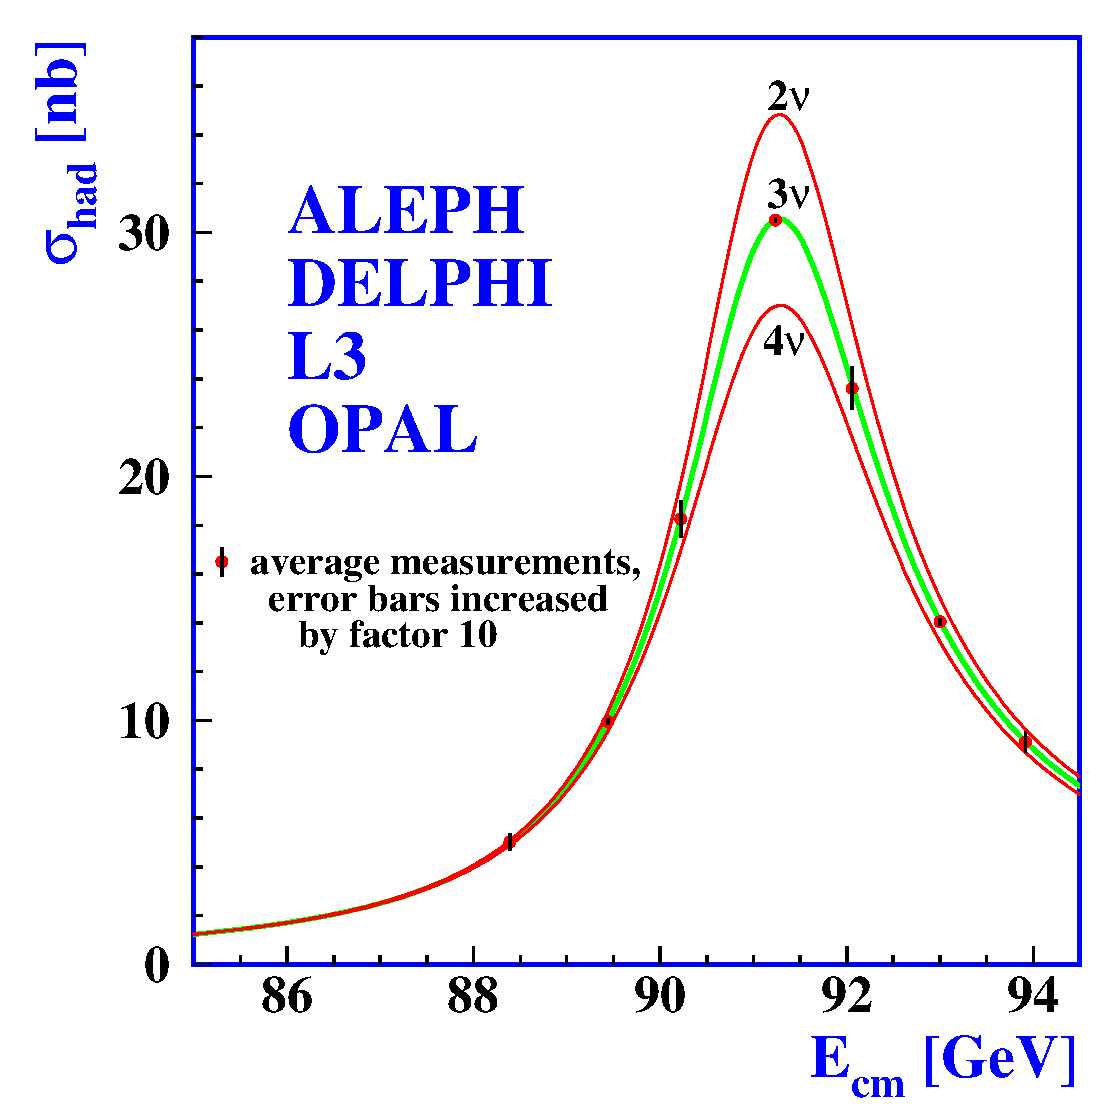
\includegraphics[width=\textwidth]{Figures/Experimental_Results/Nnu.eps}
     \caption{Measurement of the width of $Z$ boson from LEP, comparing the hypotheses of
    2, 3, or 4 neutrino generations} \label{fig:lep_Z_3_families}
   \end{subfigure}
   ~ %add desired spacing between images, e. g. ~, \quad, \qquad, \hfill etc.
      % (or a blank line to force the subfigure onto a new line)
   \begin{subfigure}[h]{0.3\textwidth}
     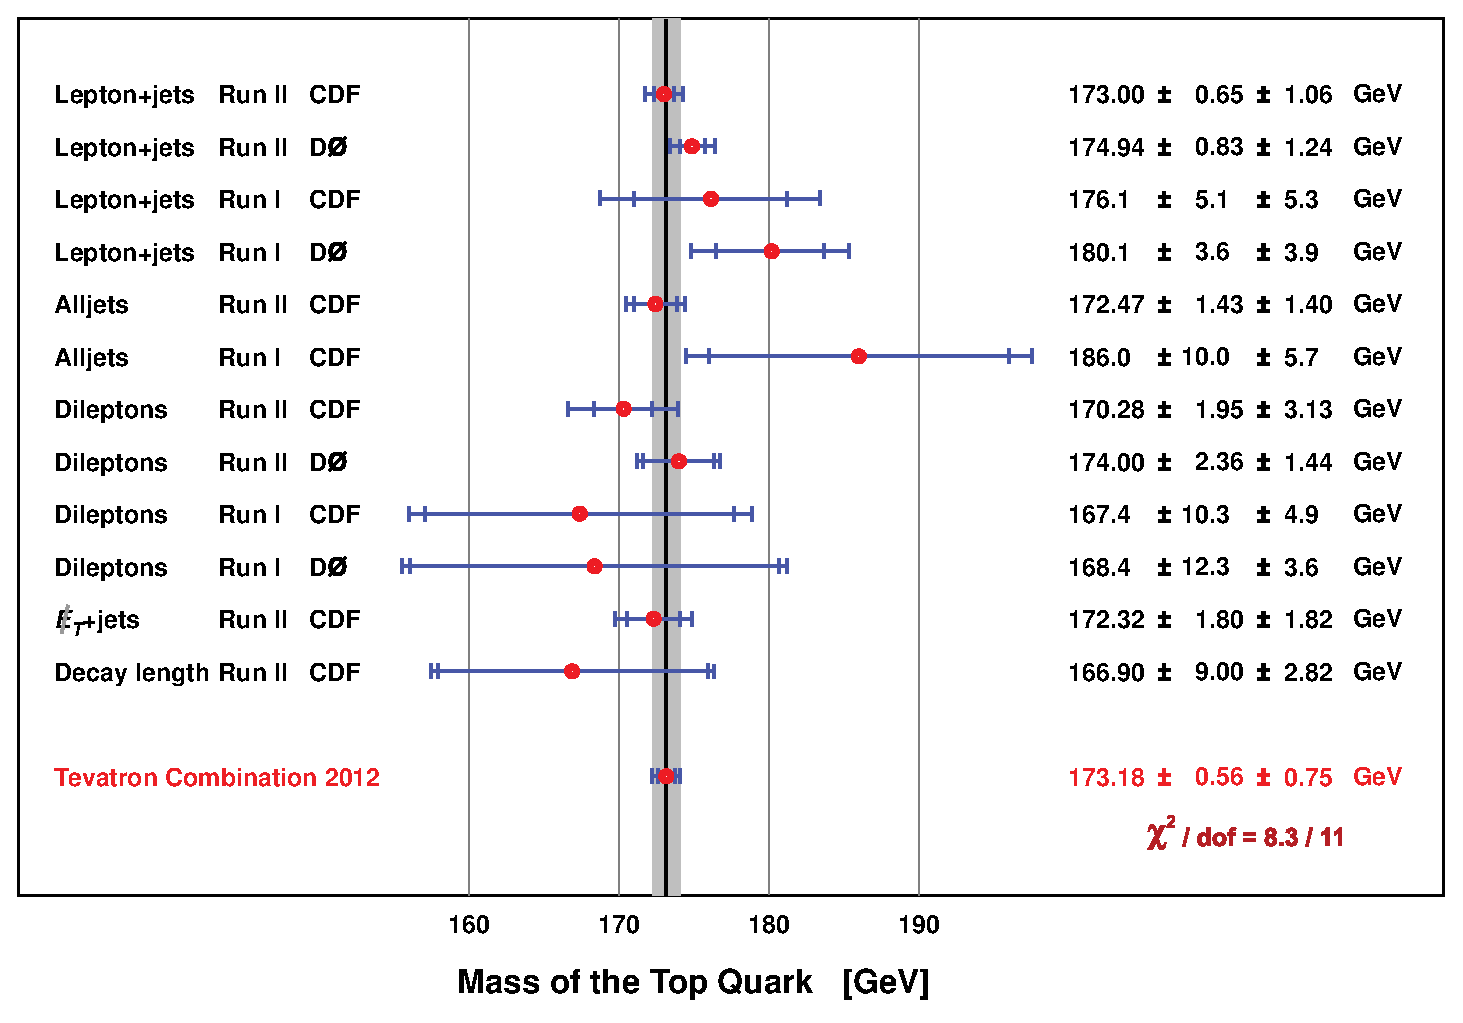
\includegraphics[width=\textwidth]{Figures/Experimental_Results/top_mass_tevatron_2012.eps}
     \caption{Measurement of the top mass from the CDF detector at the Tevatron} \label{fig:topMass_CDF}
   \end{subfigure}
   ~ %add desired spacing between images, e. g. ~, \quad, \qquad, \hfill etc.
      % (or a blank line to force the subfigure onto a new line)
   \begin{subfigure}[h]{0.3\textwidth}
     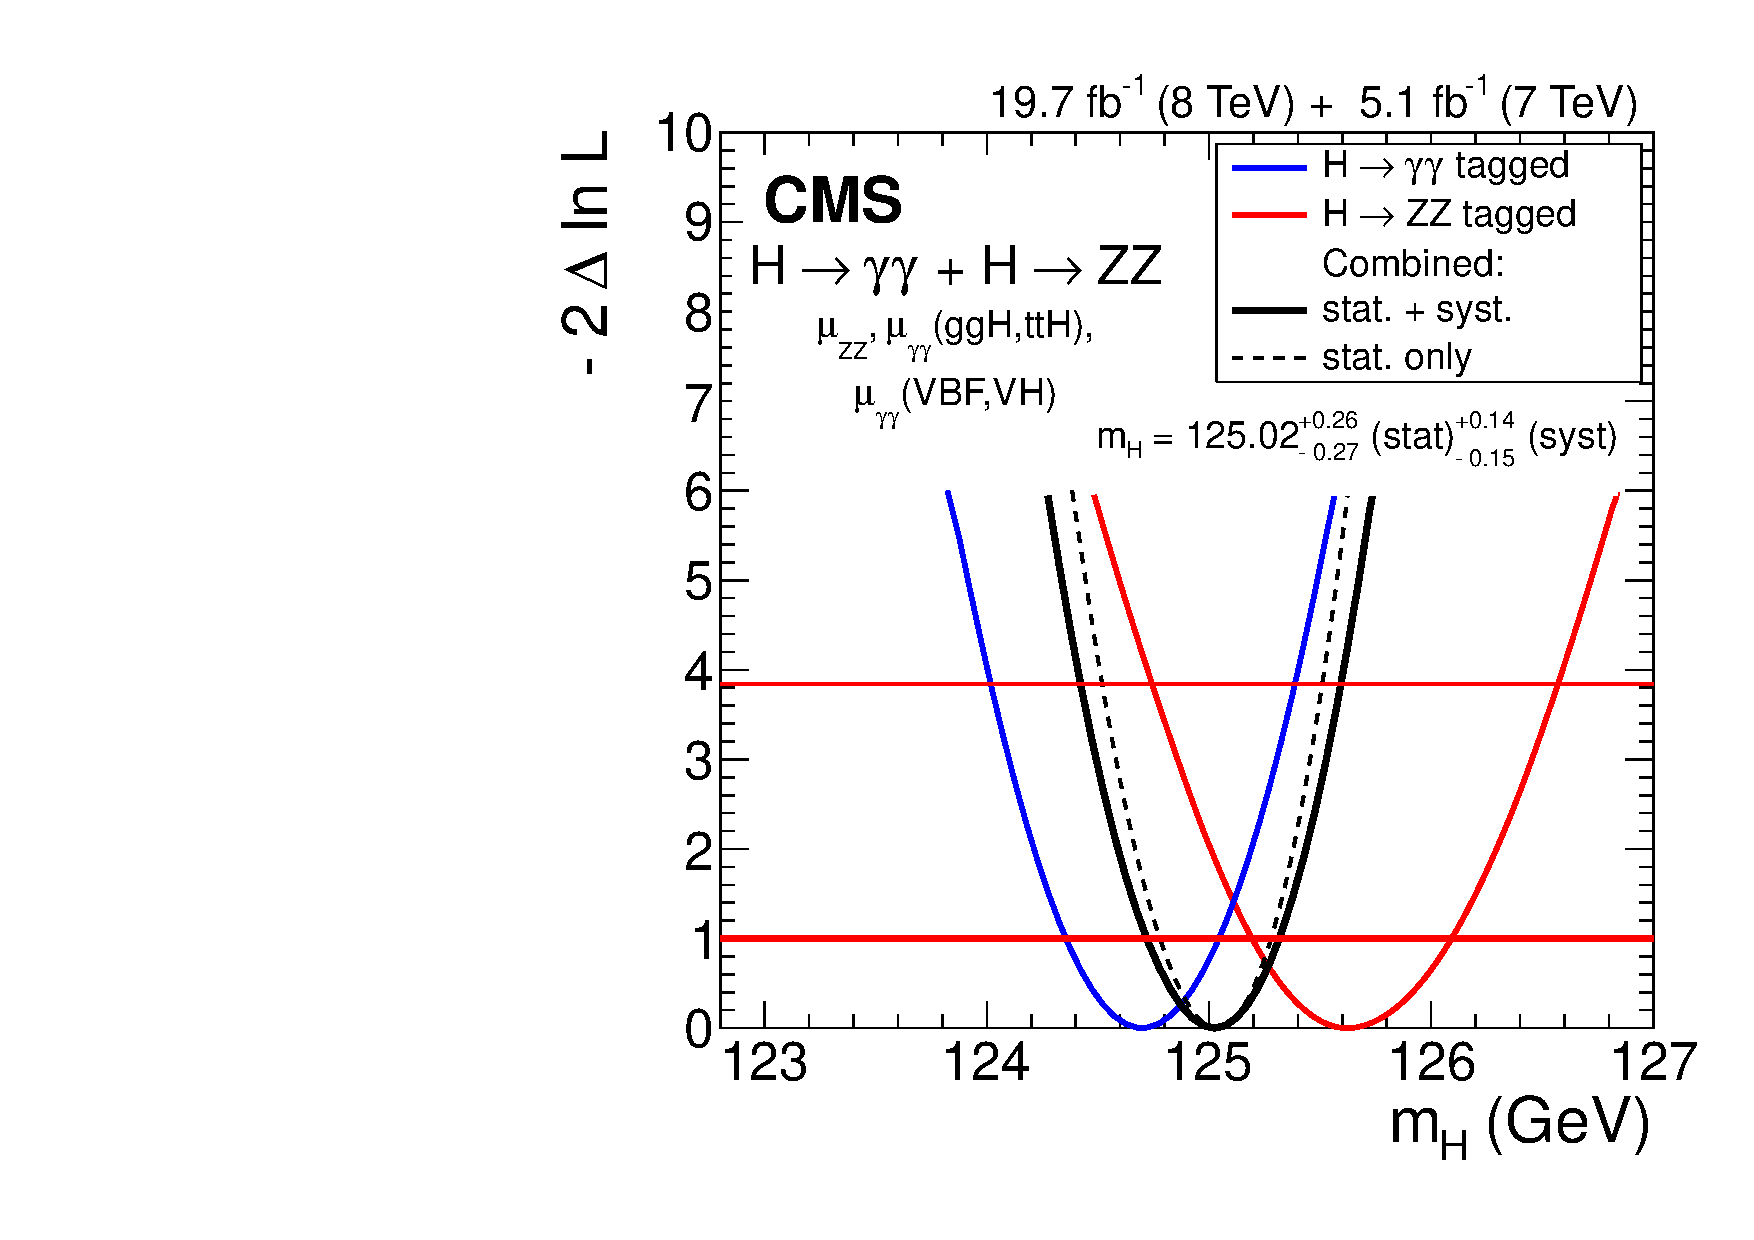
\includegraphics[width=\textwidth]{Figures/Experimental_Results/CMS_higgsMass_scan_1d_all.pdf}
     \caption{Measurement of the Higgs mass from the CMS detector at the LHC} \label{fig:topMass_CDF}
   \end{subfigure}
   \caption{Experimental milestones of the Standard Model}\label{fig:ex_milestones_sm}
\end{figure}

\noindent the experiment was also able to put stringent limits on the
existence of more than three families of leptons and quarks by
measuring the width of the $Z$ boson.  Figure
\ref{fig:ex_milestones_sm}(\subref{fig:lep_Z_3_families}) shows the
comparison of two, three, and four family hypotheses to data.   

\par Another milestone for the Standard Model occured in 1995 when the
CDF~\cite{ex:CDF_topQuark} and D0 experiments~\cite{ex:D0_topQuark} at
the Tevatron announced the observation of the top quark, with
$m_{t}\sim~176~\GeV$, in $p\bar{p}$ collisions at $\sqrt{s}=1.8~\TeV$.
Figure \ref{fig:ex_milestones_sm}(\subref{fig:topMass_CDF}) shows a
plot from 2012, the latest top quark mass measurements from CDF, which
reports a $m_{t} = 173.18 \pm 0.56 \pm 0.75~\GeV$. It was the last
quark predicted by the CKM matrix to be observed, and earned Makoto
Kobayashi and Toshihide Maskawa the nobel prize in 2008 for their work
extending the quark sector to three families and parameterizing their
electroweak mixing.    

\par Yet another milestone was reached in 2012, when the CMS and ATLAS
detectors at CERN anounced the observation of a new boson, with
characteristics strikingly similar to the elusive Higgs boson of the
SM.  Figure \ref{fig:ex_milestones_sm}(\subref{fig:topMass_CDF}) shows
the latest measurement results on the mass from the
$H\rightarrow\gamma\gamma$ and $H\rightarrow~ZZ$ channels, with a
$m_{H} = 125.02 \pm 0.27 \pm 0.15$.  One of the most important
remaining goals is to measure the couplings of this new boson to all
of the other particles in the Standard Model.  Of particular interest
is the coupling to the top-quark, since it offers the largest value of
the Higgs Yukawa coupling to measure.  This offers a test of the
nature of the coupling, as well as a probe into deviations from its
value.   


\section{Higgs Procuction in $pp$ Collisions at the LHC}
\label{higgs_production_overview}

\begin{figure}[h]
   \centering
  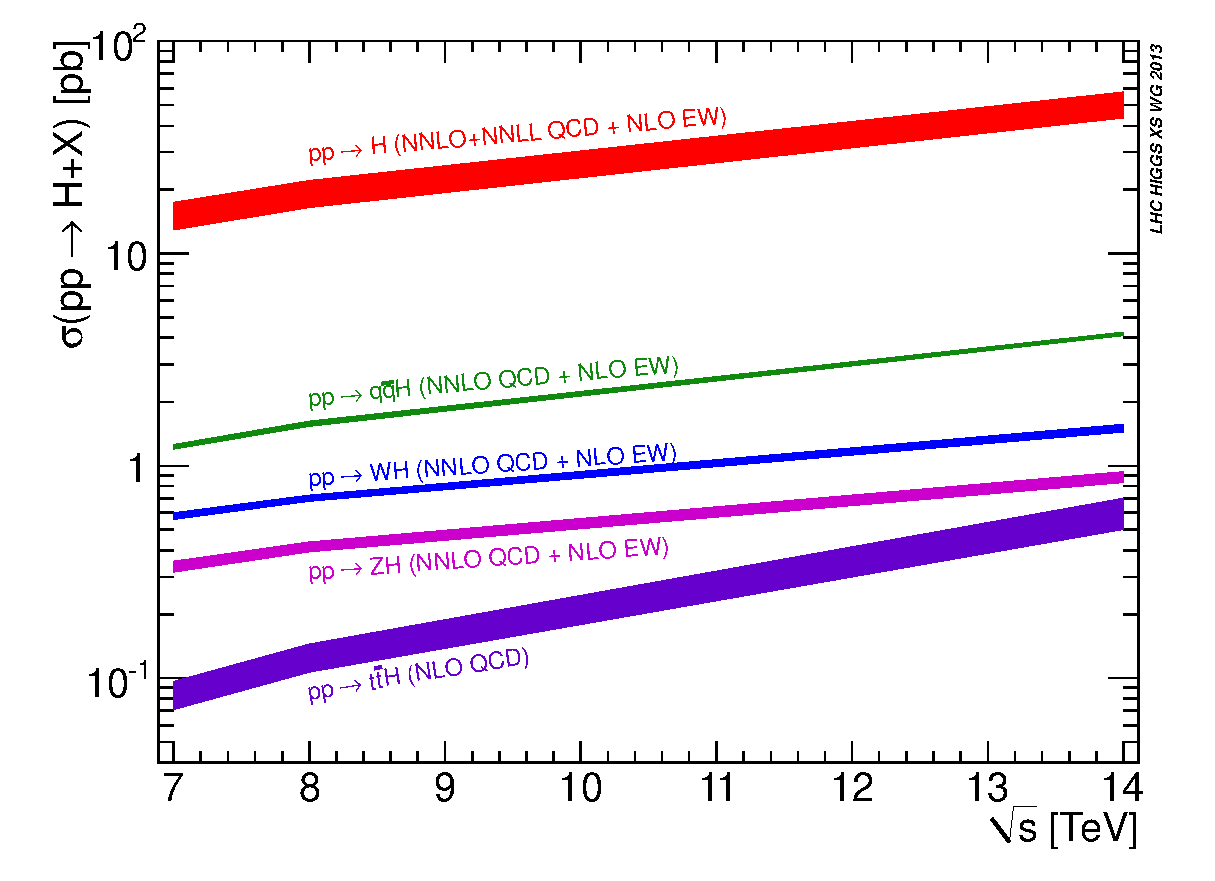
\includegraphics[width=0.5\textwidth]{Figures/Experimental_Results/Higgs_XS_7-14TeV.eps}
  \caption{Higgs production cross-sections at the LHC, for 7-14$\TeV$
    $pp$ collisions} \label{fig:Higgs_XS_7-14TeV}
\end{figure}

\par The rest of the thesis will describe the search for Higgs
boson production in proton-proton collisions at the LHC, so it will be
useful to understand the production mechanisms for the Higgs in this
scenario.  At the LHC collision energies $7-14\TeV$, there are four
dominant production mechanisms that produce Higgs events: gluon-gluon
fusion (ggf), vector-boson fusion (vbf), associated production with
vector bosons (VH), and associated production with top-quark pairs (ttH).  Figure
\ref{fig:Higgs_XS_7-14TeV} shows the relative cross sections for each
of these mechanisms.  

\begin{figure}
    \centering
    \begin{subfigure}[h]{0.3\textwidth}
        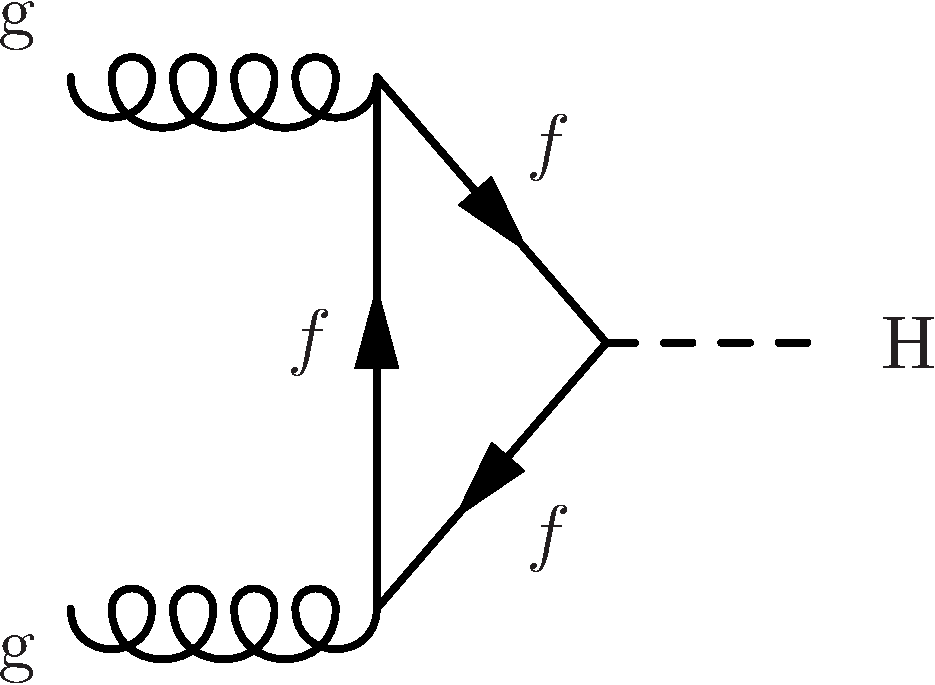
\includegraphics[width=\textwidth]{Figures/Feynman_Diagrams/higgs_production__ggf.pdf}
        \caption{Gluon-Gluon Fusion}\label{fig:higgs_production_ggf}
      \end{subfigure}
      ~ %add desired spacing between images, e. g. ~, \quad, \qquad, \hfill etc.
      % (or a blank line to force the subfigure onto a new line)
      \begin{subfigure}[h]{0.3\textwidth}
        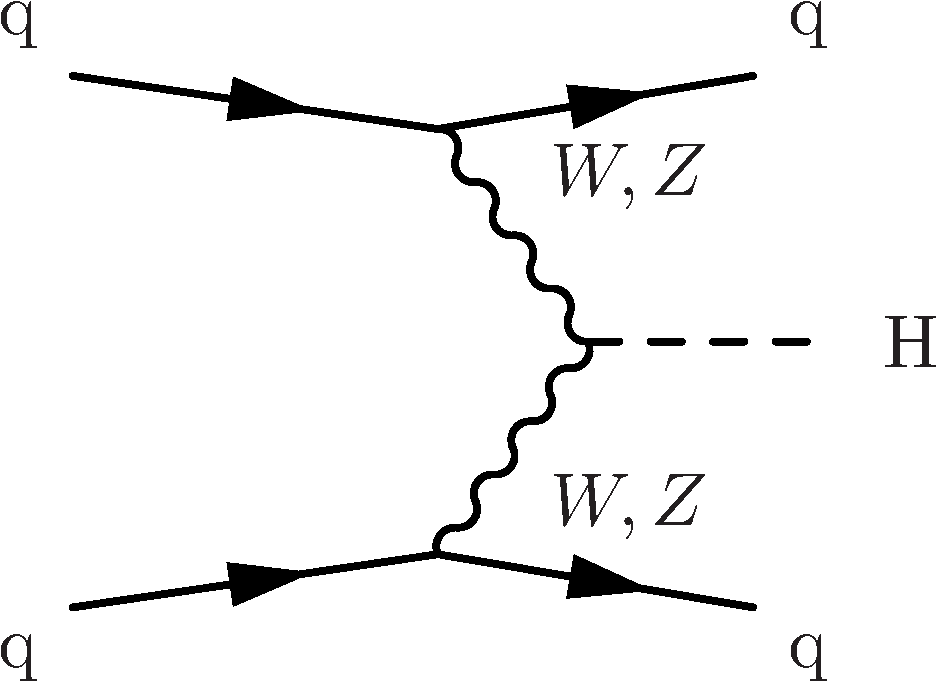
\includegraphics[width=\textwidth]{Figures/Feynman_Diagrams/higgs_production__vbf.pdf}
        \caption{Vector Boson Fusion}\label{fig:higgs_production_vbf}
      \end{subfigure}
      ~ %add desired spacing between images, e. g. ~, \quad, \qquad, \hfill etc.
      % (or a blank line to force the subfigure onto a new line)
      \begin{subfigure}[h]{0.3\textwidth}
        \includegraphics[width=\textwidth]{Figures/Feynman_Diagrams/higgs_production__vh.pdf}
        \caption{Associated Production with $W,Z$}\label{fig:higgs_production_vh}
      \end{subfigure}
      \caption{Feynman diagrams for the three largest Higgs production
        modes at the LHC} \label{fig:feynman_diagrams__higgs_production}
\end{figure}

\par Gluon-gluon fusion, which proceeds via a heavy quark
loop~\cite{th:HiggsXS_2013}, is the dominant production mechanism at
the LHC.  The QCD radiative corrections to the total cross section have been computed
at the next-to-leading order (NLO) and at the next-to-next-to-leading order (NNLO
accuracy).  The cross section for Higgs production at $m_{H} =
125\GeV$ and $\sqrt{s}=8\TeV$, the cross section is given as:
\begin{equation}\label{eq:ggf_xs}
\sigma_{ggF} = 19.27~~\pm \text{~~QCD Scale Unc.}^{+7.2\%}_{-7.8\%}~~\pm
\text{~~PDF+$\alpha_{S}$ Unc.}^{+7.4\%}_{-6.9\%}~~\pbinv
\end{equation}
\noindent Figure \ref{fig:feynman_diagrams__higgs_production}(\subref{fig:higgs_production_ggf}) shows a Feynman
diagram for this process.  The triangle loop contains all strongly
coupled fermions, which is dominated by the top-quark since the
Yukawa coupling to the Higgs is the largest.  

\par Vector boson fusion proceeds through the fusion of $W^{+}W^{-}$
or $Z^{0}Z^{0}$  gauge bosons~\cite{th:HiggsXS_2013}. The
characteristic signature of the production mode is the associated
production of two quarks, typically at a low angle relative to the
proton beam.  This process has been caclulated to NNLO for QCD and NLO
for Electroweak corrections~\cite{th:HiggsXS_2013}.  The cross section
at $m_{H} = 125\GeV$ and $\sqrt{s}=8\TeV$ is given as:
\begin{equation}\label{eq:vbf_xs}
\sigma_{VBF} = 1.653~~\pm \text{~~EW Unc.}^{+4.5\%}_{-4.5\%}~~\pm
\text{~~QCD Scale Unc.}^{+0.2\%}_{-0.2\%}~~\pm
\text{~~PDF+$\alpha_{S}$ Unc.}^{+2.6\%}_{-2.8\%}~~\pbinv 
\end{equation}
\noindent Figure
\ref{fig:feynman_diagrams__higgs_production}(\subref{fig:higgs_production_vbf})
shows a Feynman diagram for VBF production.  The large coupling to the
$W,Z$ bosons helps to make this the sub-dominant production mechanism
at the LHC.  However, the gluon content of the proton at \TeV energies
is much larger than that of the valence quarks, thus the relative
suppression.  

\par The third largest production mechanism for Higgs bosons at the
LHC is through associated production with a $W$ or $Z$
boson~\cite{th:HiggsXS_2013}.  It has been calculated to NNLO for QCD
and NLO for Electroweak corrections. This process is also sometimes
referred to as, Higgstrahlung, since it resemble the bremstrahlung
process of an electron radiating a photon. The higher order
electroweak corrections are similar to that of the Drell-Yan, so much
of the technology to compute the cross-section can be borrowed from
existing EW calculations.  The cross section for $m_{H} = 125\GeV$ and
$\sqrt{s}=8\TeV$ is:  
\begin{equation}\label{eq:vh_xs}
\begin{aligned}
\sigma_{WH} =&~ 0.7046~~\pm \text{~~QCD Scale Unc.}^{+1.0\%}_{-1.0\%}~~\pm
\text{~~PDF+$\alpha_{S}$ Unc.}^{+2.3\%}_{-2.3\%}~~\pbinv \\
\sigma_{ZH} =&~ 0.4153~~\pm \text{~~QCD Scale Unc.}^{+3.1\%}_{-3.1\%}~~\pm
\text{~~PDF+$\alpha_{S}$ Unc.}^{+2.5\%}_{-2.5\%}~~\pbinv 
\end{aligned}
\end{equation}
\noindent Figure
\ref{fig:feynman_diagrams__higgs_production}(\subref{fig:higgs_production_vh})
shows the Feynman diagram for VH production.  This channel is most
useful for identifying hadronic decays of the Higgs, since the
associated gague boson can decay to leptons, giving a strong kinematic
handle over backgrounds that would normally overwhelm a similar search
in the ggF channel.  


\section{\ttH Production in $pp$ Collisions at the LHC}
\label{ttH_production_overview}

\begin{figure}[h]
   \centering
  \includegraphics[width=0.3\textwidth]{Figures/Feynman_Diagrams/higgs_production__ttH.pdf}
  \caption{Feynman diagram for \ttH production} \label{fd:ttH_simple}
\end{figure}

\par The \ttH production mode is the fourth largest production mode at
the LHC~\cite{th:HiggsXS_2013}.  This production mode has been
calculated to NLO in
QCD~\cite{tthXS_NLO_BeenakkerEtAl_1}~\cite{tthXS_NLO_BeenakkerEtAl_2}
and has been studied recently with the state of the art NLO tools
using the aMC@NLO~\cite{tthXS_aMCatNLO_Frederix} and POWHEG
(PYTHIA+HERWIG)~\cite{tthXS_powheg_Garzelli} frameworks. Studies have
also been performed interfacing NLO QCD studies
~\cite{tthXS_NLO_Dawson} with the Sherpa parton shower
framework~\cite{tthXS_sherpa_Gleisberg}.  Additional studies on the
effects of spin correlations with the aMC@NLO and Madspin framework
have also been performed~\cite{tthXS_aMCatNLO_madspin_Artoisenet}.  

\par  It has been found that the additional of NLO effects increases
the cross-section relative to LO by $\sim20\%$.  The largest
theoretical uncertainty comes from the variation of the
renormalization and factorization scale, the QCD coupling $\alpha_{S}$,
and the PDF uncertainty.  The renomarlization and factorization scales
are set to $\mu_{R} = \mu_{F} = (1/2)(m_{T} + m_{T} + m_{H})$ and are
varied by a factor of 2 to determine the cross-section's dependence on
these parameters.  Three different PDF sets,  MSTW2008, CTEQ6.6, and
NNPDF2.0 were used with the appropriate corresponding values of
$\alpha_{S}$ to determine the combined effect of varying
PDF+$\alpha_{S}$.  The cross section for $m_{H} = 125\GeV$ and
$\sqrt{s}=8\TeV$ is given by:
\begin{equation}\label{eq:tth_xs}
\sigma_{ttH} = 0.1293~~\pm \text{~~QCD Scale Unc.}^{+3.8\%}_{-9.3\%}~~\pm
\text{~~PDF+$\alpha_{S}$ Unc.}^{+8.1\%}_{-8.1\%}~~\pbinv
\end{equation}

\noindent A search for the Higgs in this production mode is
additionally challenging due to this large $\sim10\%$ error on the
theoretical cross-section.  Figure \ref{fd:ttH_simple} shows a Feynman
diagram for this process before the branching of the top-quarks or
Higgs to final states.  

\par When asking for the Higgs to decay to b-quark
pairs, yet another complication arrises when trying to identify which
b-quarks came from a top decay or from a Higgs decay.  For example, in
the semileptonic decay of top quarks, there will be four b-quarks, and
two light-flavor quarks in the final state.  This means there are 15
(six choose four) possibilities to associate quarks to the top
system.  Although this is potentially constrained by b-tagging, and
kinematic requirements (such as forming the top or $W$ masses), the
number of remaining possibilites smears out the resolution on peaking
variables such as the invariant mass of b-quark pairs.  


\section{Background Processes to \ttH}
\label{ttH_backgrounds_overview}

\begin{figure}{h}
    \centering
    \begin{subfigure}[h]{0.4\textwidth}
        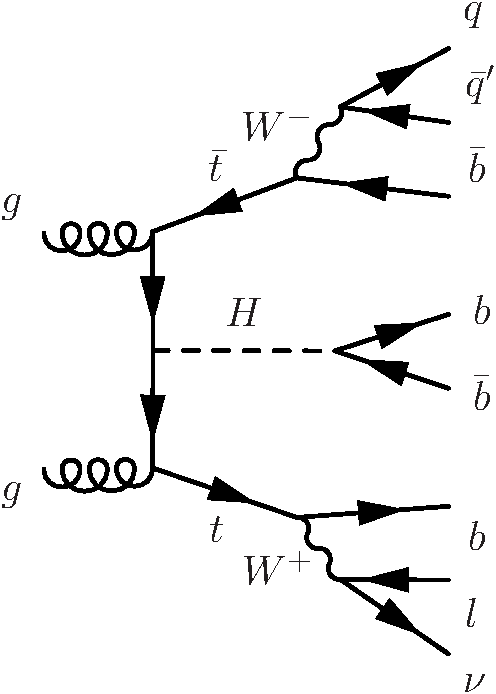
\includegraphics[width=\textwidth]{Figures/Feynman_Diagrams/higgs_production__tth_semileptonic.pdf}
        \caption{Semileptonic \ttH, with $H\rightarrow~b\bar{b}$}\label{fig:higgs_production_tth_semileptonic}
      \end{subfigure}
      ~ %add desired spacing between images, e. g. ~, \quad, \qquad, \hfill etc.
      % (or a blank line to force the subfigure onto a new line)
      \begin{subfigure}[h]{0.4\textwidth}
        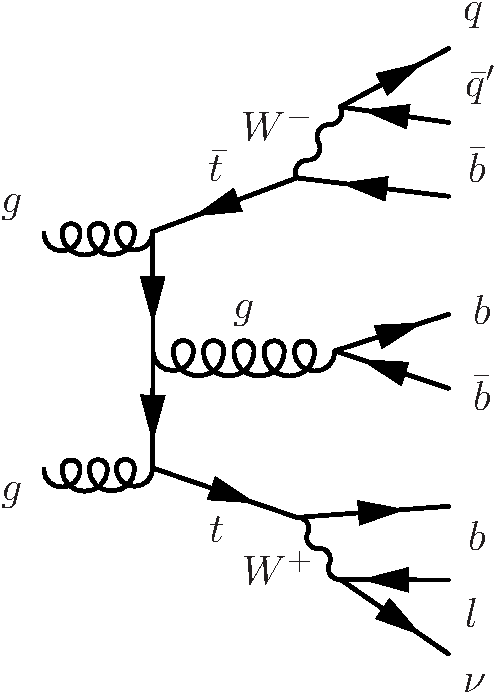
\includegraphics[width=\textwidth]{Figures/Feynman_Diagrams/backgrounds__ttbar_plus_bbar_semileptonic.pdf}
        \caption{Semileptonic \ttbb}\label{fig:higgs_production_vbf}
      \end{subfigure}
      \caption{Feynman diagrams for the semileptonic \ttH process and
        its irreducible background, \ttbb } \label{fig:feynman_diagrams__tth_vs_ttbb_semilep}
\end{figure}

\par The dominant background for \ttH production of top-quark pairs
with additional ISR/FSR jets, \ttjets.  The irreducable component of
this background is comes when the extra radiation produces a final
state with two additional b-quarks, \ttbb.  Figure
\ref{fig:feynman_diagrams__tth_vs_ttbb_semilep} compares the Feyman
diagrams for the semileptonic decays of \ttH and \ttbb.  

\par Additional difficulties come from the theoretical uncertainty on
the \ttbb background~\cite{th:HiggsXS_2013}.  The process has been
calcualted to NLO QCD in Sherpa~\cite{tthXS_sherpa_Gleisberg} and
OpenLoops~\cite{ttbbXS_openloops_Cascioli}~\cite{ttbbXS_openloops_help1_Krauss}~\cite{ttbbXS_openloops_help2_Gleisberg}.
It has been found that depending on selection cuts, and use of NLO PDF
inputs, the difference between LO and NLO calculations on the cross
section can be anywhere from $0.99\%$ to $1.96\%$.  

\par The light flavor component of the \ttjets background also enters
in the selection when any of the jets from the $t\bar{t}$ system or
extra radiation are misidentified as $b$-jets.  The cross-section for
the \ttjets process is $\sim245\pbinv$.  This is a factor of 1800, so
even if a b-tagging algorithm performs with a $1\%$ mis-identification
rate of light-jets, there will still be a large contribution from this
process that will leave a very similar signature in the detector as
\ttH. 

\begin{figure}{h}
    \centering
    \begin{subfigure}[h]{0.4\textwidth}
        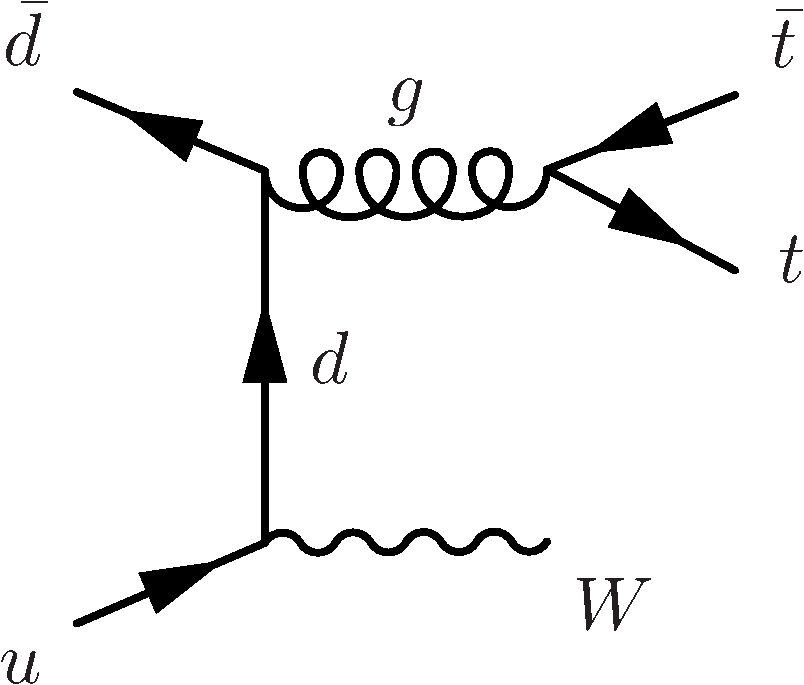
\includegraphics[width=\textwidth]{Figures/Feynman_Diagrams/backgrounds__ttbar_plus_W.pdf}
        \caption{The \ttW background}\label{fd:ttW}
      \end{subfigure}
      ~ %add desired spacing between images, e. g. ~, \quad, \qquad, \hfill etc.
      % (or a blank line to force the subfigure onto a new line)
      \begin{subfigure}[h]{0.4\textwidth}
        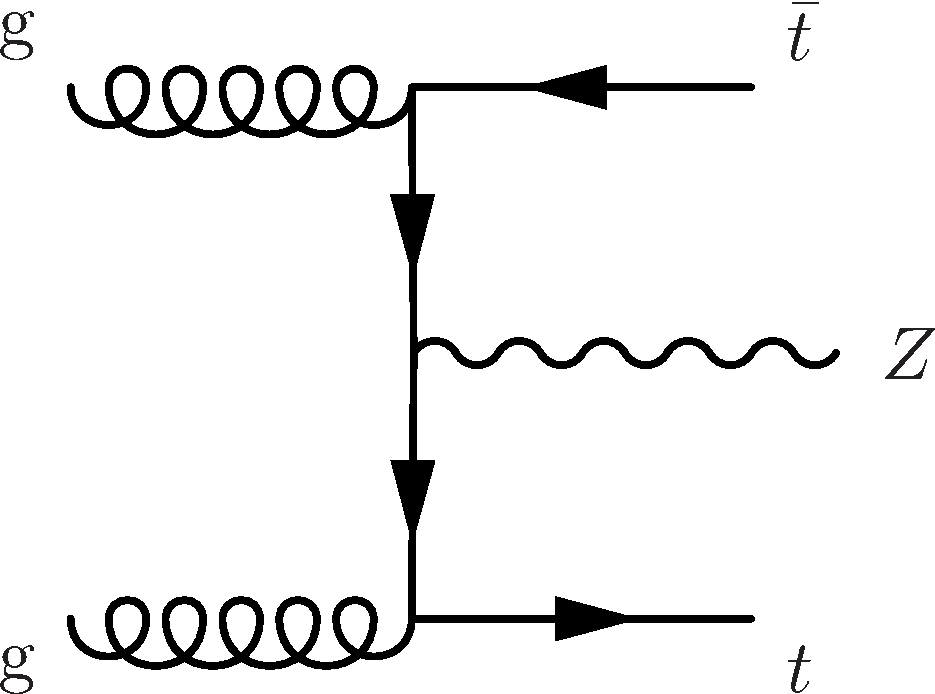
\includegraphics[width=\textwidth]{Figures/Feynman_Diagrams/backgrounds__ttbar_plus_Z.pdf}
        \caption{The \ttZ background}\label{fd:ttZ}
      \end{subfigure}
      \caption{Feynman diagrams for the \ttW and \ttZ background processes} \label{fig:feynman_diagrams__ttW_ttZ}
\end{figure}

\par The next largest background is the production of vector bosons in
association with top-quark pairs, \ttW and \ttZ.  Figure
\ref{fig:feynman_diagrams__ttW_ttZ} shows Feynman diagrams from these
two processes.  They have cross-sections of $\sigma_{ttW}=0.249\pbinv$
and $\sigma_{ttZ}=0.208\pbinv$, which are only a factor of $\sim$2
greater than the \ttH process.  These processes can enter the
semileptonic \ttH selection by a semileptonic \ttbar decay, while the
vector bosons decay to quarks, or through a hadronic \ttbar decay,
while the vector bosons decay to quarks, and in the case of \ttZ, of
the leptons is not identified in the reconstruction.  

\begin{figure}{h}
    \centering
    \begin{subfigure}[h]{0.3\textwidth}
        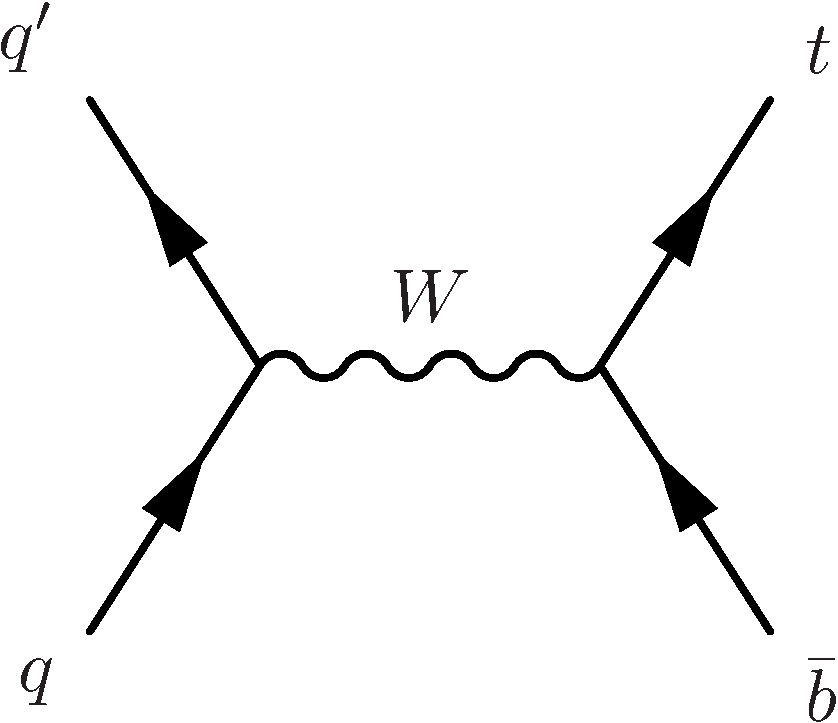
\includegraphics[width=\textwidth]{Figures/Feynman_Diagrams/backgrounds_singleT_sChan.pdf}
        \caption{Single $t$, s-channel}\label{fd:t_sChan}
      \end{subfigure}
      ~ %add desired spacing between images, e. g. ~, \quad, \qquad, \hfill etc.
      % (or a blank line to force the subfigure onto a new line)
      \begin{subfigure}[h]{0.3\textwidth}
        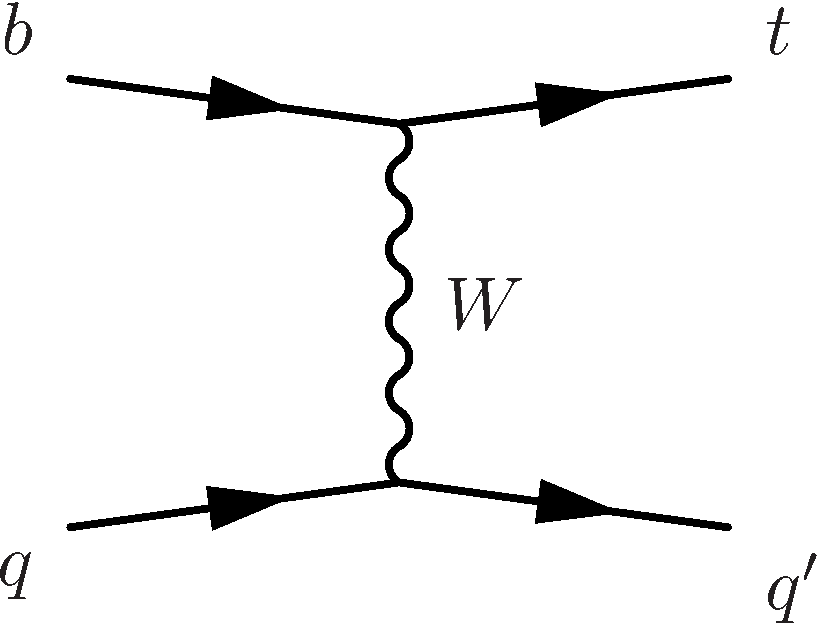
\includegraphics[width=\textwidth]{Figures/Feynman_Diagrams/backgrounds_singleT_tChan.pdf}
        \caption{Single $t$, t-channel}\label{fd:t_tChan}
      \end{subfigure}
      ~ %add desired spacing between images, e. g. ~, \quad, \qquad, \hfill etc.
      % (or a blank line to force the subfigure onto a new line)
      \begin{subfigure}[h]{0.3\textwidth}
        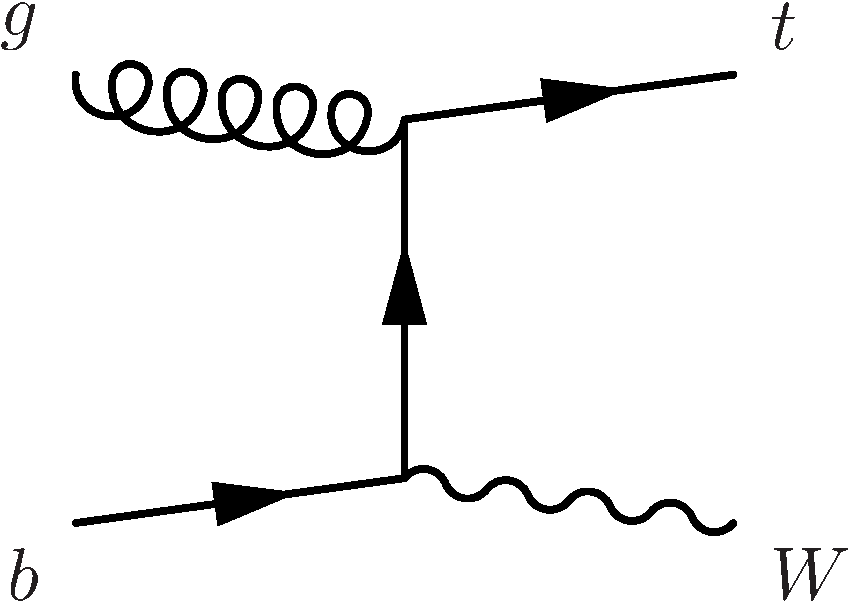
\includegraphics[width=\textwidth]{Figures/Feynman_Diagrams/backgrounds_singleT_tWChan.pdf}
        \caption{Single $t$, tW-channel}\label{fd:t_tWChan}
      \end{subfigure}
      \caption{Feynman diagrams for the single $t$ s,t, and t$W$ background processes} \label{fig:feynman_diagrams__singleT_t_s_tW_channels}
\end{figure}


\par Single top production is also an important background to consider
in a search for \ttH production.  Figure
\ref{fig:feynman_diagrams__singleT_t_s_tW_channels} shows Feynman
diagrams for this process.  It does not have as large of a
contribution as the other backgrounds, since it requires addional
radiation in order to have a similar final state jet multiplicity as
\ttH.  However, since a top-quark is still involved in the process,
the final state kinematics of its decay products will be very similar.
 Single $t$ production has a cross section of $\sigma_{t}=71.3\pbinv$,
 while Single $\bar{t}$ production has a cross section of
 $\sigma_{\bar{t}}=43.6\pbinv$, due to charge asymmetry of the valence
 quarks of the proton

\begin{figure}{h}
    \centering
    \begin{subfigure}[h]{0.3\textwidth}
        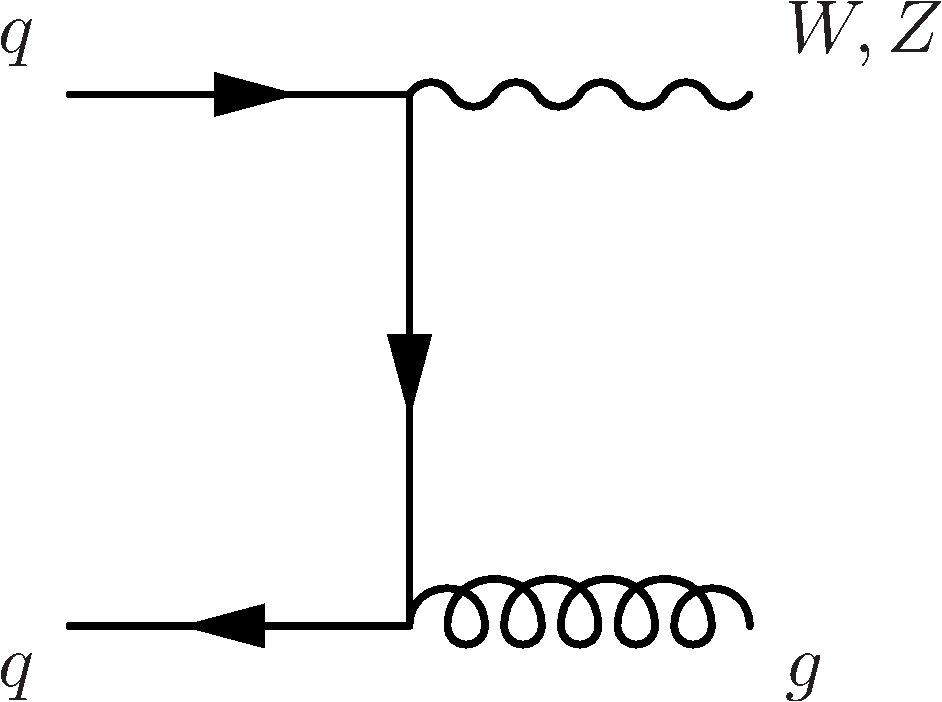
\includegraphics[width=\textwidth]{Figures/Feynman_Diagrams/backgrounds__VplusJets.pdf}
        \caption{$W,Z$ plus jets}\label{fd:t_tChan}
      \end{subfigure}
      ~ %add desired spacing between images, e. g. ~, \quad, \qquad, \hfill etc.
      % (or a blank line to force the subfigure onto a new line)
      \begin{subfigure}[h]{0.3\textwidth}
        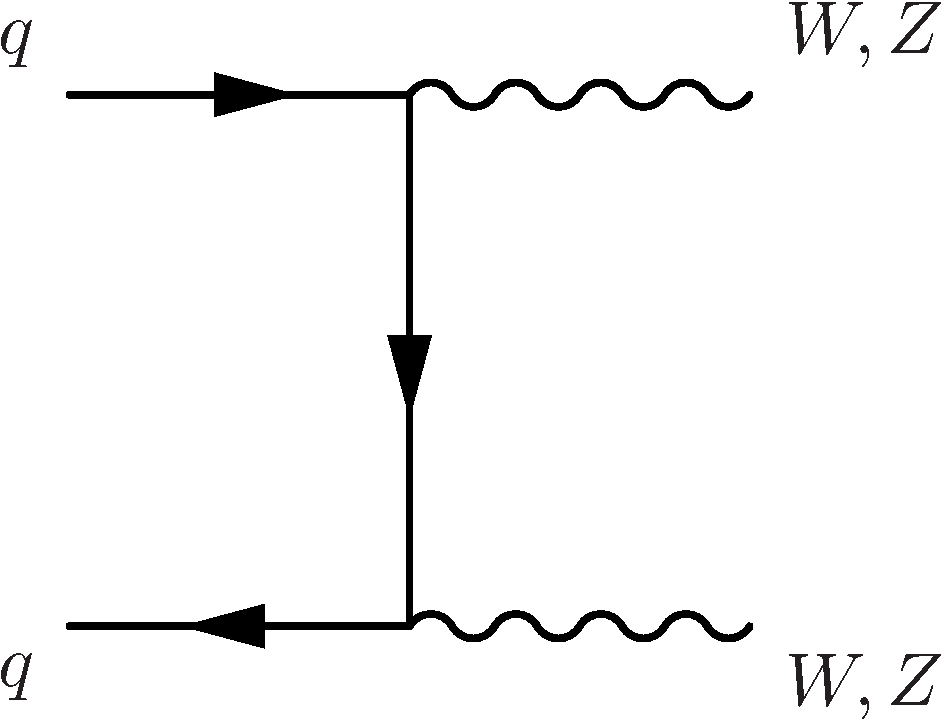
\includegraphics[width=\textwidth]{Figures/Feynman_Diagrams/backgrounds__VV.pdf}
        \caption{DiBoson Production}\label{fd:VV}
      \end{subfigure}
      \caption{Feynman diagrams for the $W,Z$ plus jets, and diBoson
        ($WW$, $WZ$, $ZZ$) production.} \label{fig:feynman_diagrams__Vjets__VV}
\end{figure}

\par The last backgorunds to consider are the electroweak production
of $W$ and $Z$ bosons in association with jets, as well as $WW$, $WZ$, and
$ZZ$ pairs in association with jets.  Figure
\ref{fig:feynman_diagrams__Vjets_VV} shows the Feynman diagrams for
these processes, where the $V$, stands in for wither $W$ or $Z$
bosons.  For a semileptonic selection of \ttH events, $Z$ plus jets
events enter from a mis-identification of one of the leptons from the
$Z$ boson decay.  Extra FSR/ISR radiation is also to leave a similar
signature in the signal region of a \ttH search, so it mainly
contributes to control regions of the data.  

\section{Potential BSM Effects on~\ttH~production}
\label{bsm_effects_overview}

\par The phenomological motivation for the existence of physics beyond
the Standard Model come from the observation of phenomenon or states
of matter not described by the theory.  Observations of the cosmic miscrowave background
from the Plank telescope have estimated that only $\sim5\%$ of the
observable universe is composed of ordinary
matter~\cite{BSM_Planck}. The remaining composition is divided between  
Dark Matter ($\sim27\%$, and $\sim68\%$ respecitvely).  Evidence for
Dark Matter also comes from discrepencies between the observed
rotational velocities of galaxies, and the observed mass
distributions, suggesting the presence of additional form of matter
which does not interact
electromagnetically~\cite{BSM_Rubin_DM_GalaxyRotations}.

\par Additionally, in 1998, the Super-Kamiokande experiment proved that
neutrinos oscillated between flavors, implying indirectly that they
also have mass~\cite{BSM_superK}.  This is something not described in
the Standard Model of physics.  Due to their neutral charge, these
particles  are extremely difficult to detect, so experiments have only
been able to measure differences in the mass squared between the three
mass eigenstates.  In 2005, the KamLAND experiment reported
$|{\Delta}m^{2}_{12}=0.000079
eV^{2}|$~\cite{BSM_neutrinoDeltaM12_kamland}.  In 2006, the MINOS
experiment reported
$|{\Delta}m_{23}=0.0027 eV^{2}|$~\cite{BSM_neutrinoDeltaM23_minos}.

\par One of the largest theoretical problems with the Standard Model,
comes the mechanism which made it all possible- the Higgs.  In
equation \ref{eq:ewk_lagrangian_unbroken} there are terms that couple
the Higgs boson to itself, $-{\lambda}vh^{3}$, and
$-\frac{1}{4}{\lambda}h^{4}$.  When computing NLO effects, these terms
lead to a divergence in the Higgs mass, when considering the effect of
a loop of fermions on the Higgs propagator.  The correctios are of the form ${\Delta}m_{H} =
-\frac{\lambda_{f}^{2}}{8\pi^{2}}\Lambda_{UV}$.  Where $\Lambda_{UV}$
is the high energy cut off for the theory, which in the limit of a
perfect theory, should extend to infinity.  This is known as the
hierarchy problem.  

\par Beyond the Standard Model physics is a term that describes
extensions of the Standard Model in order to describe the observed
phenomenon.  For the neutrino oscilations, a solution similar to CKM
matrix has been proposed, the Pontecorvo–Maki–Nakagawa–Sakata (PMNS)
matrix.  This proposes that the mass eigenstates of the neutrino are
linear combinations of the weak eigenstates, allowing for the mixing
of flavors.  Current experiments now seek to measure the free
parameters of this matrix.  

\begin{figure}[h]
   \centering
  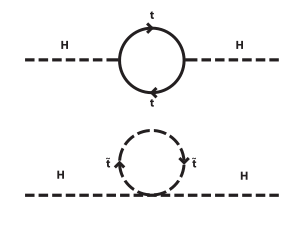
\includegraphics[width=0.5\textwidth]{Figures/Basic_Diagrams/hierarchy_problem_susy_solution.png}
  \caption{The cancellation of the divergent Higgs mass from a loop of
  top-quarks is cancelled by a loop of supersymmetric top-quarks,
  stop-quarks,} \label{fig:hierarchy_problem}
\end{figure}

\par Both the dark matter and hierarchy problems suffer in the fact
that there is no clear model, such as the PMNS matrix, to provide a
theoretical solution.  Out of the plethora of theories that attempt to
solve these problems, supersymmetry (SUSY) is the most popular in the
theoretical and experimental community.  It suggests that there is a
broken symmetry between fermions and bosons, and introduces a partner
to each Standard Model particle with a spin quantum number less
1/2~\cite{Martin_SUSY_primer}.  For the hierarch problem, this
provides a set of particles to cancel out the divergences in the NLO
corrections to the Higgs mass.  Figure \ref{fig:hierarchy_problem}
shows the Feynmann diagrams for a supersymmetric top-quark, or stop
quark, that would cancel the divergent contribution from the Standard
Model top quark.  Depending on the specific form of the SUSY model,
the stop quarks can potentially couple directly or indirectly to the
top-quark, producing them at a higer rate during $pp$ collisions.
This would effect the number of observed events making it into the
\ttH~selection.  

\par A number of extensions to the SM also involve introducing new
top-like particles into the theory.  Vector-like quarks would be spin
1/2 particles that transform as triplets under the $SU(3)$ color group
and whose left and right-handed components have the same  
color and electroweak quantum
numbers~\cite{VectorLikeQuarks_Aguilar-Saavedra}.  These objects are
common to several different types of models.  Little Higgs
models~\cite{BSM_littleHiggs_Burdman}~\cite{BSM_littleHiggs_Perelstein}~\cite{BSM_littleHiggs_PhysRevD.74.055001}, 
models with extra
dimensions~\cite{BSM_extraD_Cheng:1999bg}~\cite{BSM_extraD_Carena:2006bn},
top-color models~\cite{BSM_topColor_Hill:1991at}, and composite Higgs
models~\cite{BSM_composite_Higgs_Contino:2006qr}, include a
vector-like top partner,$ t^{\prime}$ that decays to a top-quark and
either a Higgs, $W$, or $Z$ particle.  Both $t^{\prime}t^{\prime}$
pair production and $t^{\prime}t$ production would yield the ttH final
state, or at least one indistinguishable detector signature.  \ttH
search can provide indirect limits on these models, by observing an
excess or lack thereof of \ttH events, without having to directly
construct a $t^{\prime}$ resonance.  


      

\chapter{The Large Hadron Collider}
\label{lhc_overview}

\begin{figure}[h]
   \centering
  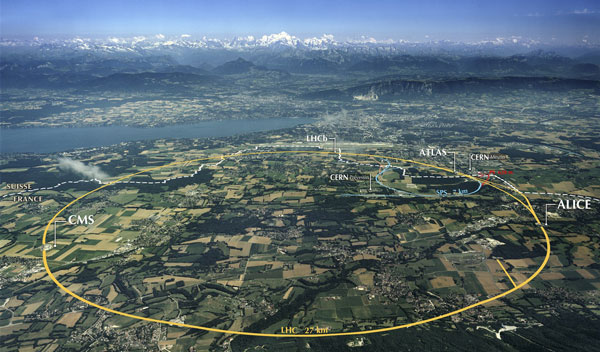
\includegraphics[width=1.0\textwidth]{Figures/LHC_Diagrams/LHC_Aerial_View.jpg}
  \caption{Aerial view of the LHC complex, spanning the French-Swiss border~\cite{LHC:Aerial_View}} \label{fig:lhc_aerial_with_labels}
\end{figure}

\par The \acrfull{lhc}, is a superconducting, proton-proton,
accelerator and collider operated by the \acrfull{cern} laboratory in
Geneva, Switzerland~\cite{lhc:machine_description}.  Figure
\ref{fig:lhc_aerial_with_labels} shows an aerial view of the LHC
complex, with the main laboratory camus being labeled as CERN, with
four of the detector experiments being labeled as ALICE, ATLAS, CMS,
and LHCb.  Three smaller experiments, not pictured, also use the LHC
ring, and are TOTEM, LHCf, and MOeDAL.  It was designed to elucidate
the mechanism of electroweak symmetry breaking and explore \TeV scale
of particle physics.  As such, it is required to produce a large
number of high center-of-mass energy events.  The high center-of-mass
energy allows the creation of heavy particles, while a large
luminosity allows for the creation of rare processes.  The number of events
produced at a collider is a product of the luminosity of the collider
and the total cross-section for the objects being collided.  

\begin{equation}\label{eq:Nevents}
N_{events} = L\sigma_{event}
\end{equation}

\noindent  The cross-section, $\sigma_{event}$, can be estimated from the
theory of the Standard Model as described in section
\ref{qft_overview} and validated by measuremnt at detectors, such as
CMS, as shown in section \ref{ttH_backgrounds_overview}.  The
luminosity is a control of the experiment, and for Guassian
distributed beams, is given by the equation:

\begin{equation}\label{eq:lumi}
L = \frac{ N_{b}^{2}n_{b}f_{rev}\gamma_{r}
}{ 4\pi\epsilon_{n}\beta^{\ast} }F
\end{equation}

\noindent The parameters of this equation and their value for the LHC
is as follows:
\begin{itemize}
\item $N_{b}$ - Number of of particles per bunch, squared since there
  are two beams.  The mechanism of acheiving such high energies is
  based in Radio-Frequency (RF) cavity technology, which clusters the
  protons together into packets, which are all accelerated and
  collided together.  For the LHC, $N_{b} = 1.15 x 10^{11}$.
\item $n_{b}$ - Number of bunches per beam.  The maximum design for
  the LHC allows for $n_{b} = 2808$ bunches, however in practice,
  lower number of bunches have been run with in order to create more
  time between bunch crossings.  
\item $f_{rev}$ - Revolution frequency of the protons in the LHC
  ring.  This is determined by ring circumference, and for the LHC,
  $f_{rev} = 11.2$ kHz. 
\item $\gamma_{r}$ - This is the relativistic gamma-factor, determined
  by the speed, and thus the center of mass energy of the collisions.  
\item $\epsilon_{n}$ - This is the normalized transverse emmitance of
  the beam, which describes the RMS spread of the beam in its
  transverse plane.  For the LHC $\epsilon_{n} = 3.75~\mu$m.  
\item $\beta^{\ast}$ - Is the minimum of the $\beta$ function, which
  is defined as the square of the transverse beamsize divided by
  $\epsilon_{n}$.  It is minimized at interaction regions, where the
  beams are being squeezed into the smallest region possible, to
  maximize the probability of protons colliding during each bunch
  crossing.  For the LHC, $\beta^{\ast} = 0.55$ 
\item $F$ - This is the efficiency for having the two beams head-on,
  and is determined by the crossing angle at which the two
  counter-rotating beams meet each other.  
\end{itemize}

\noindent The LHC is designed to deliver a maximum luminosity of L =
10$^{34}$cm$^{2}$s$^{1}$ to the CMS and ATLAS experiments, with a
maximum center-of-mass energy of $\sqrt{s}=14\TeV$.  


\begin{figure}[h]
   \centering
  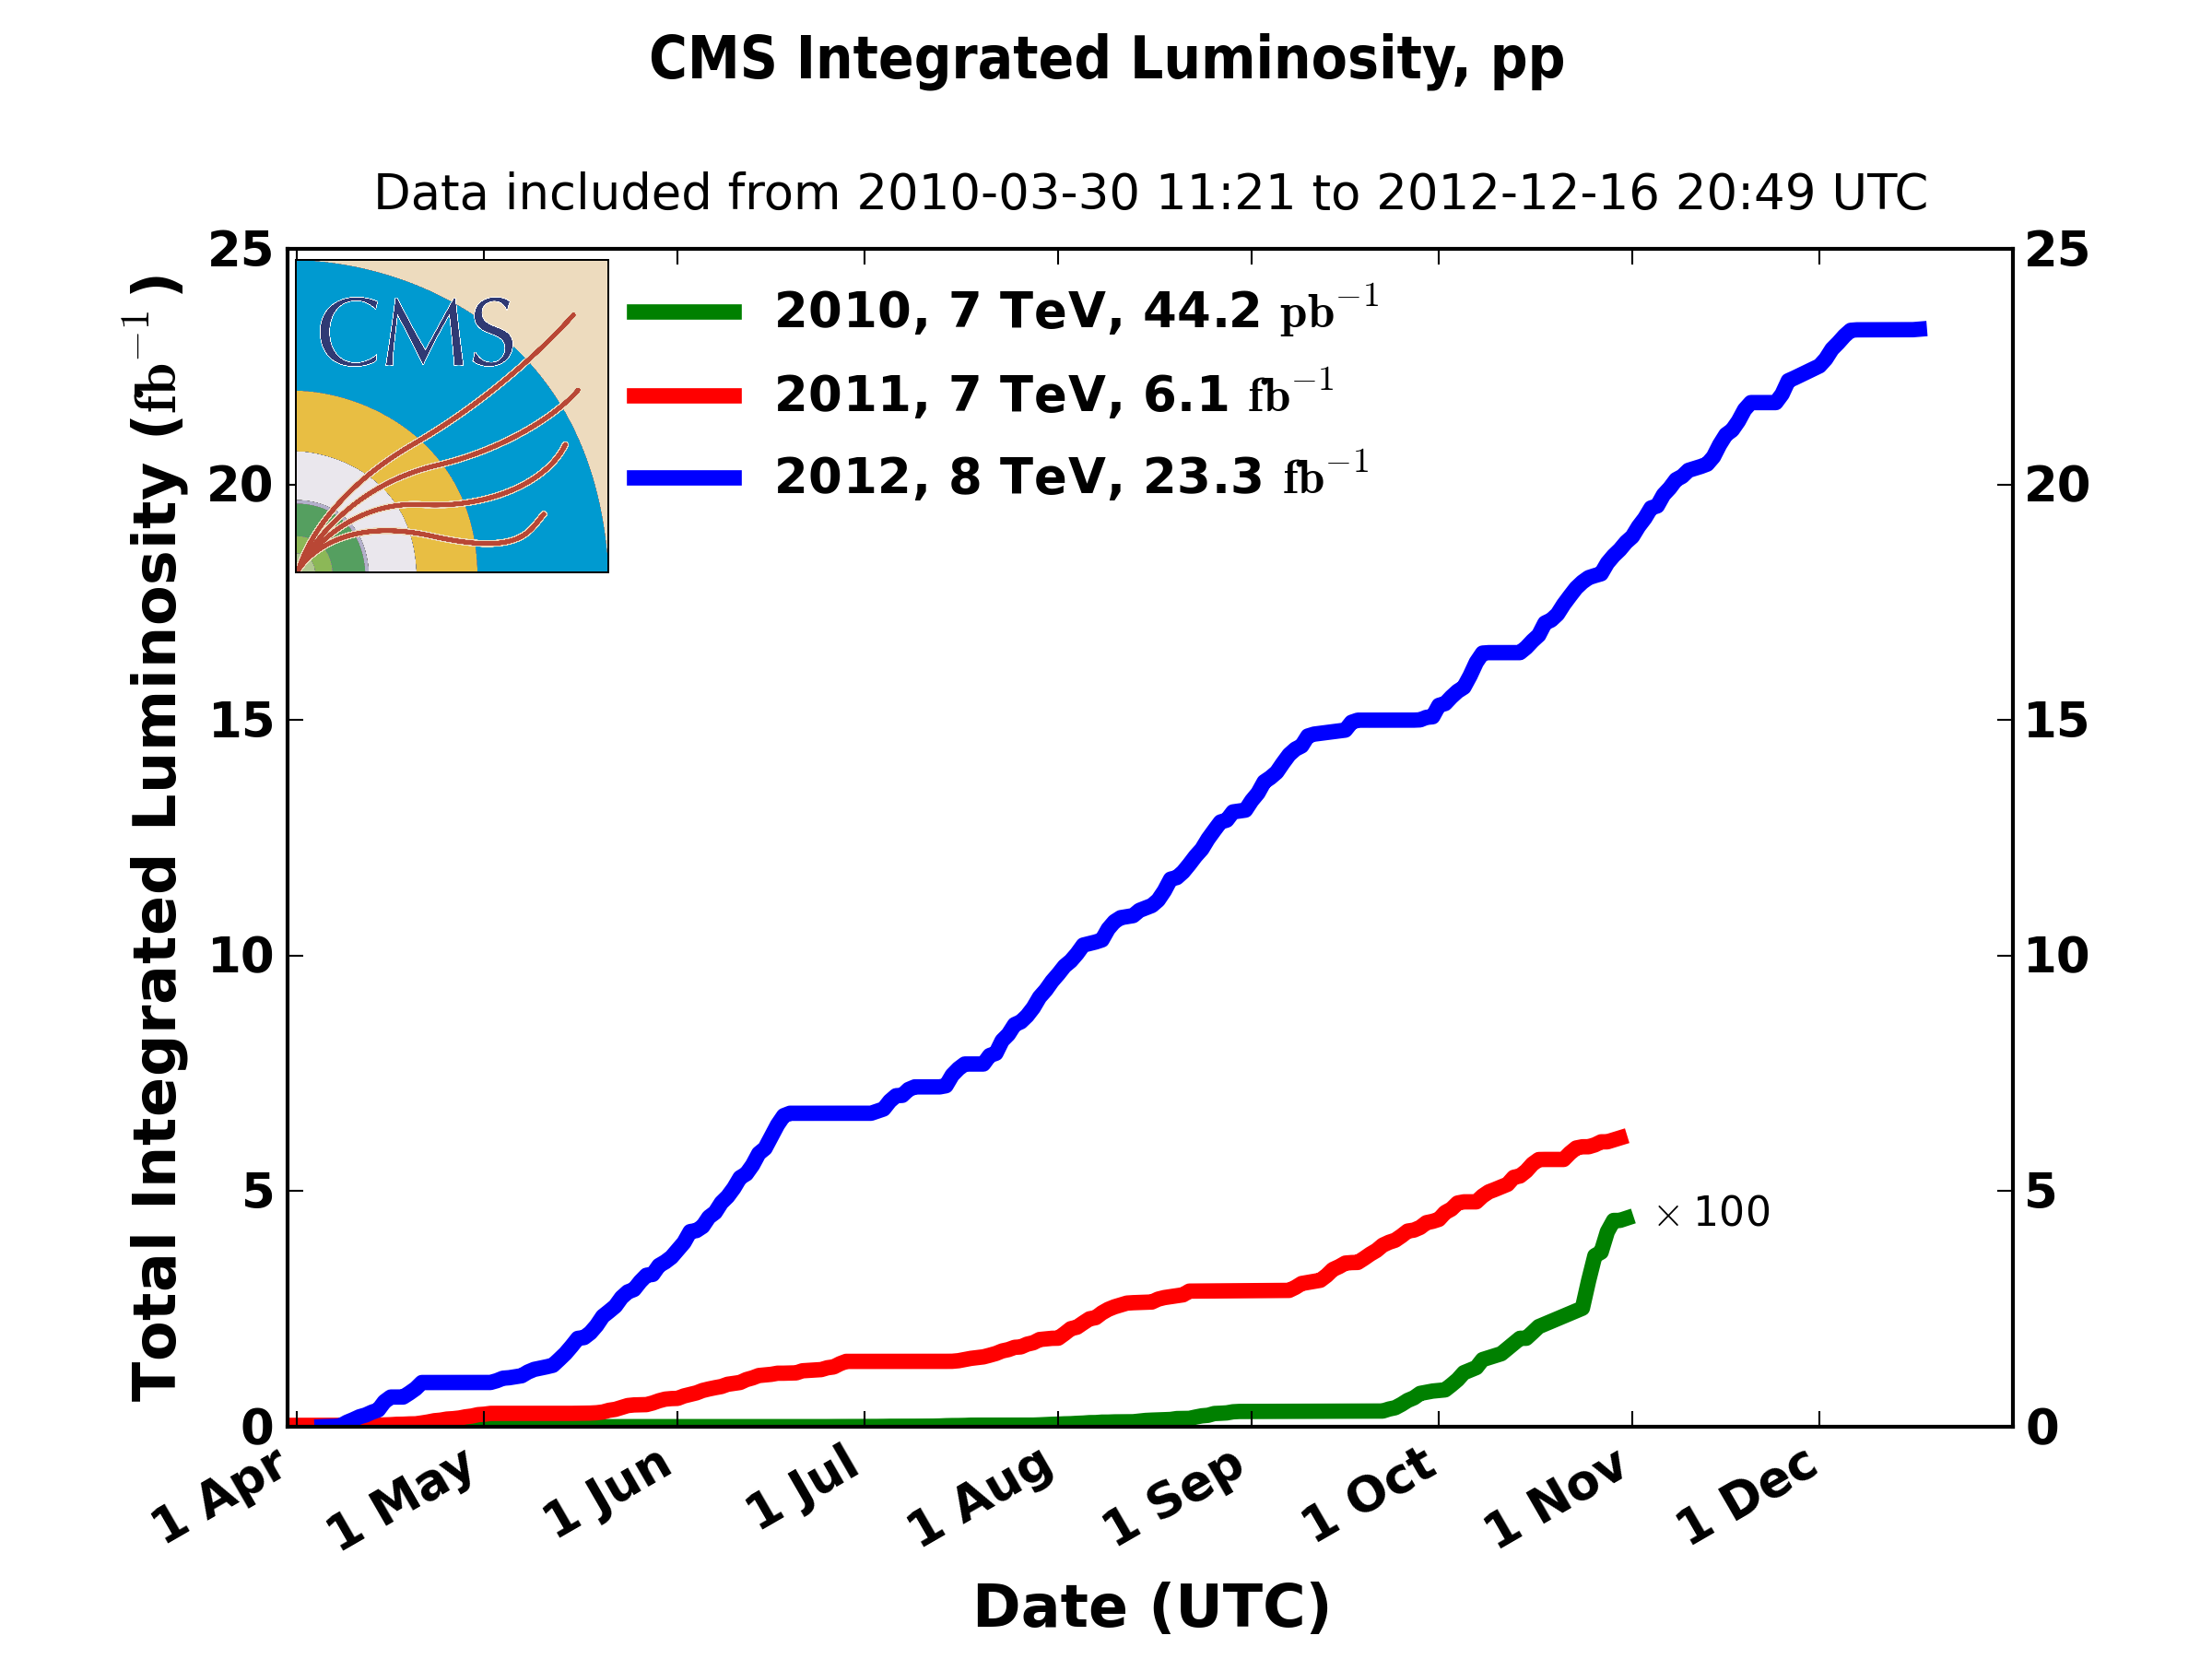
\includegraphics[width=0.8\textwidth]{Figures/Experimental_Results/CMS__int_lumi_cumulative_pp_2.png}
  \caption{Integrated Luminosity delived to the CMS experiment from 2010-12} \label{fig:cms_integrated_lumi}
\end{figure}

\par In 2010-11, the LHC ran at center-of-mass energy,
$\sqrt{s}=7\TeV$ and delivered $\sim6\fbinv$ of data to the CMS
experiment.  In 2012, it ran at $\sqrt{s}=8\TeV$ and collected
$\sim23\fbinv$.  Figure \ref{fig:cms_integrated_lumi} shows a diagram of
the luminosity collected as a function of time for each year running.  

\par The next sections will describe the LHC accelerator complex, the
chain of events leading up to collisions of protons at the LHC, and
the associated technologies that allow for the control and operation
of the high-energy, high-luminosity beams that allow the CMS and ATLAS
experiments to search for heavy particles and rare-processes.  


\section{The LHC Accelerator Complex}
\label{lhc_injection_chain}

\par The main LHC ring is a 26.7 km tunnel, that is 45 m to 170 m
underneath the surface of the earth, with 1.4$\%$ slope towards Lake
Leman.  It extends accross the French-Swiss border, into the French
coutnryside.  The tunnel was originally constructed between 1984 and 1989 for
the Large Electron Positron (LEP) experiment that is famous for it's
precision mesaurements of several Standard Model
parameters~\cite{lhc:machine_description}.  The choice to build the
ring underground was driven by real estate costs, but the underground
setting also provides natural radiation shielding from the beamline
and greatly reduces the impact of cosmic radiation on the detectors.  

\begin{figure}[h]
   \centering
  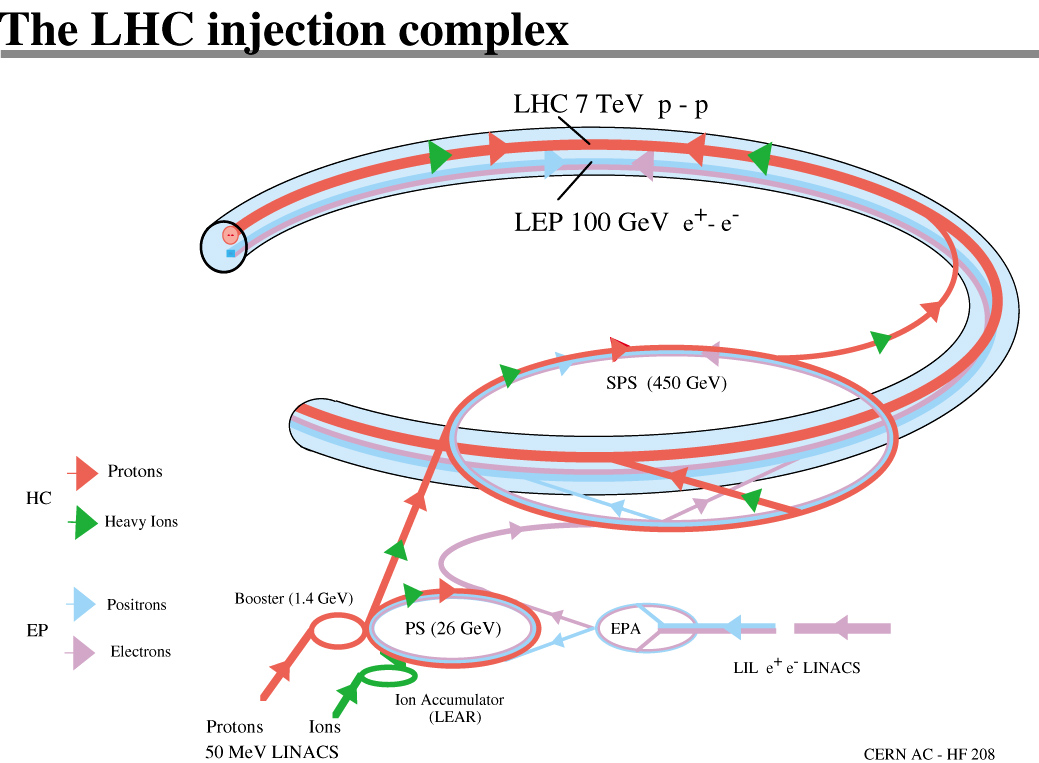
\includegraphics[width=0.8\textwidth]{Figures/LHC_Diagrams/LHC_injection_complex.jpg}
  \caption{The LHC accelerator complex, taking protons from a bottle
    of Hydrogen at the Linac2, all the way to the LHC
    ring} \label{fig:lhc_accelerator_complex}
\end{figure}

\par The LHC also utilizes the existing accelerator complex from the
LEP expermiment, which is shown in figure
\ref{fig:lhc_accelerator_complex}.  The complex is composed a series
of increasingly powerful accelerators that gradually increase the
energy of the protons.  

\begin{figure}{h}
    \centering
    \begin{subfigure}[h]{0.4\textwidth}
        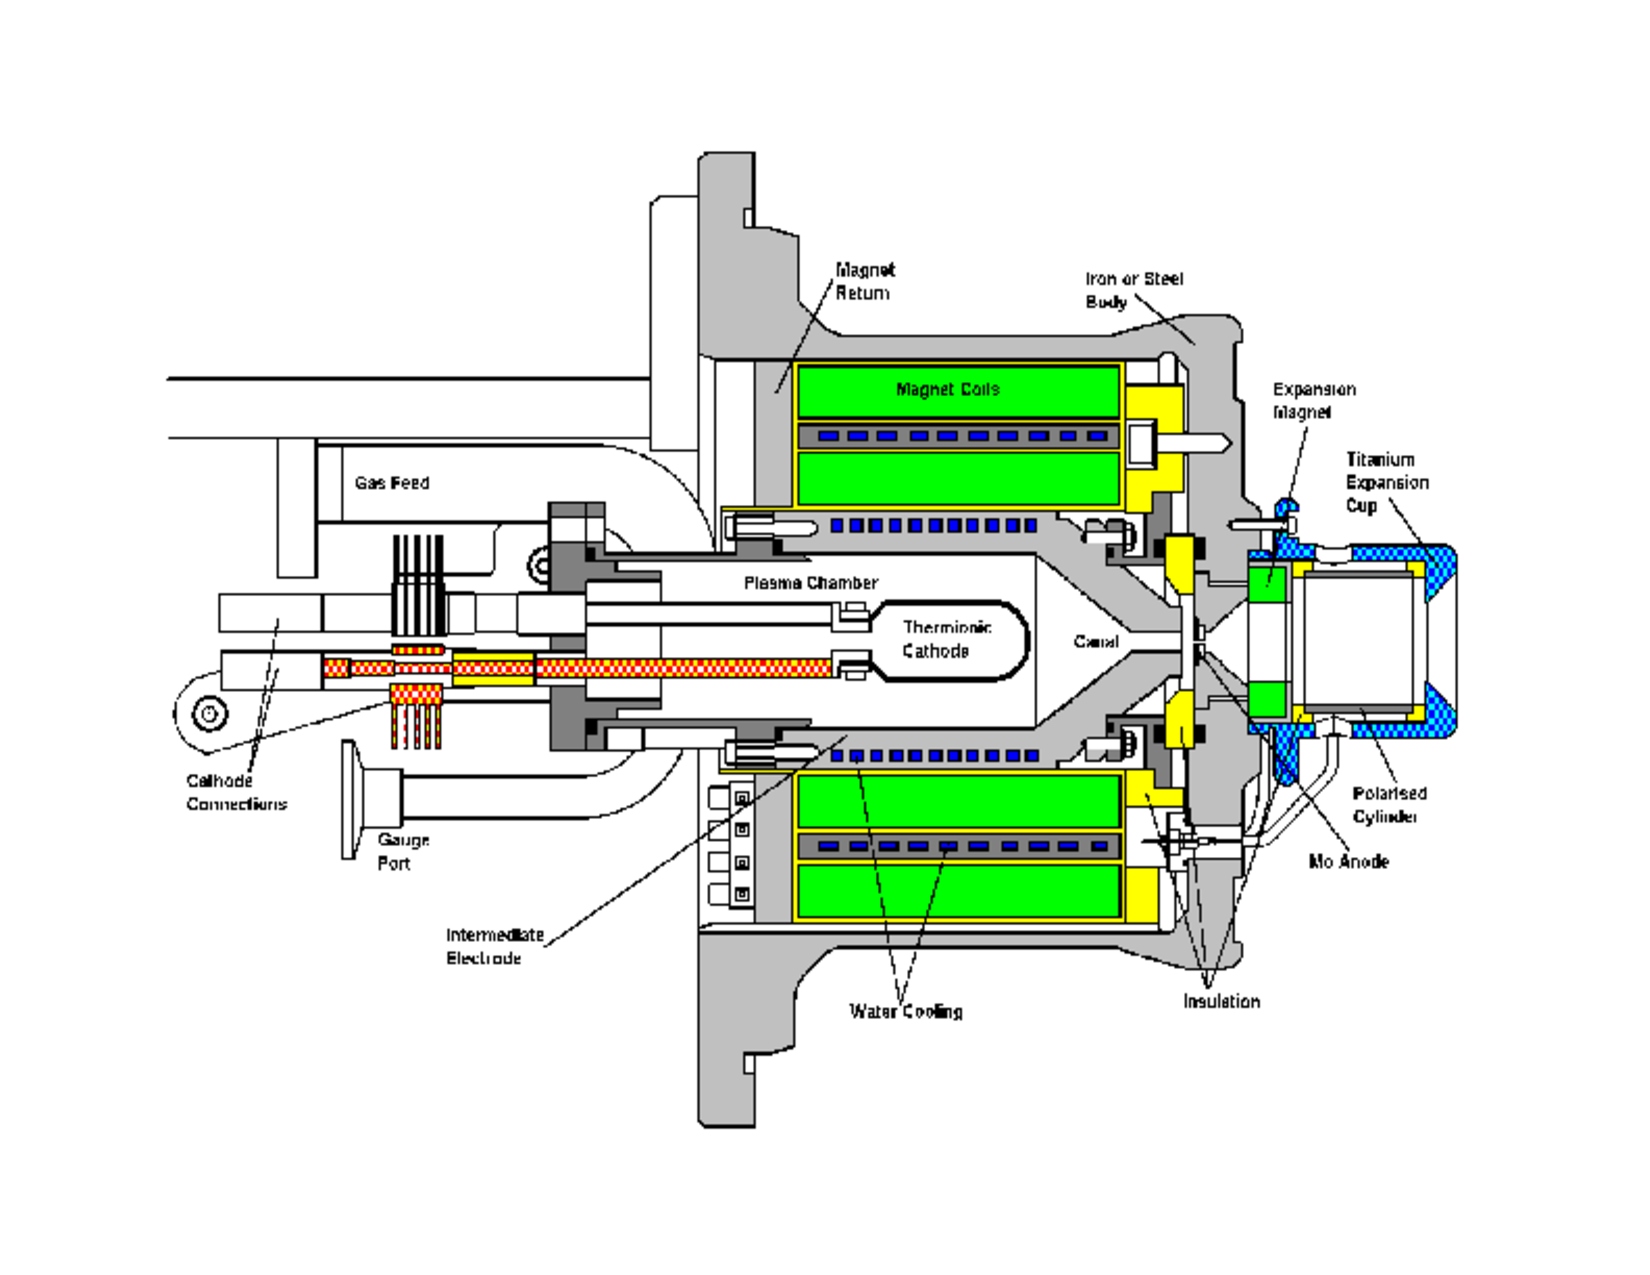
\includegraphics[width=\textwidth]{Figures/LHC_Diagrams/LHC__Linac2__Duoplasmatron_Schematic.pdf}
        \caption{Schematic of the duoplasmatron ion source, which
          creates a proton beam from source bottle of Hyrdogen}\label{fig:duoplasmatron_schematic}
      \end{subfigure}
      ~ %add desired spacing between images, e. g. ~, \quad, \qquad, \hfill etc.
      % (or a blank line to force the subfigure onto a new line)
      \begin{subfigure}[h]{0.4\textwidth}
        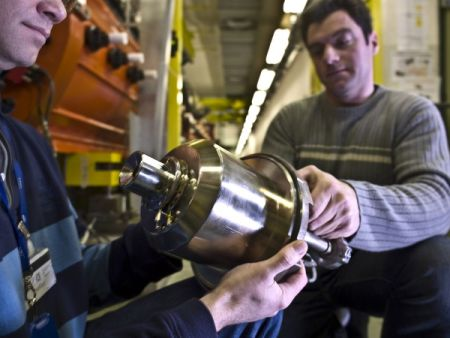
\includegraphics[width=\textwidth]{Figures/LHC_Diagrams/LHC__Linac2__Duoplasmatron__CF002521-ProtonSourceDuoplasmatronRichardChristianss.jpg}
        \caption{The Duoplasmatron used in the Linac2 at CERN, the
          source of the LHC proton beam}\label{fig:duoplasmatron_actual}
      \end{subfigure}
       ~ %add desired spacing between images, e. g. ~, \quad, \qquad, \hfill etc.
      % (or a blank line to force the subfigure onto a new line)
      \begin{subfigure}[h]{0.4\textwidth}
        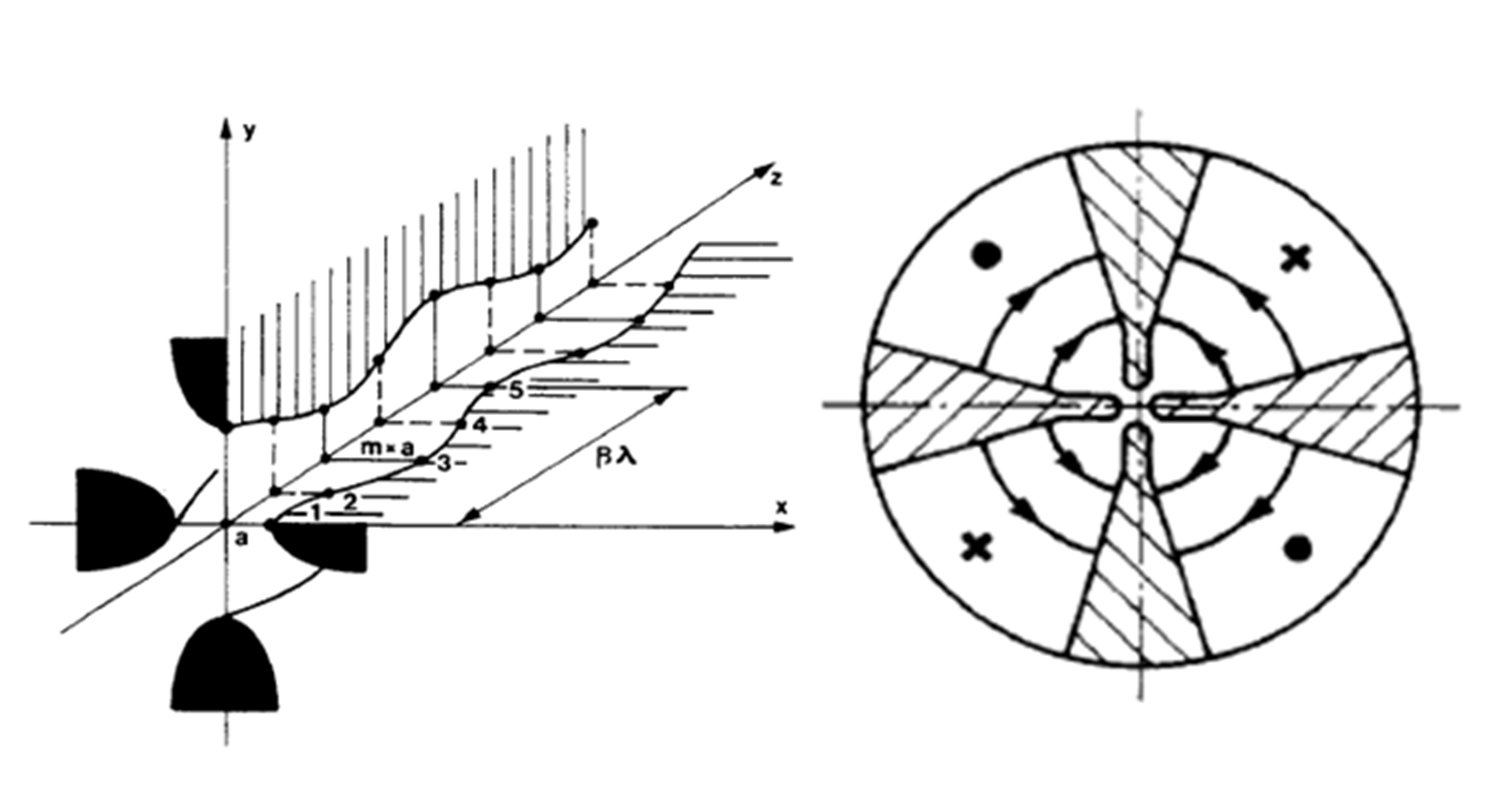
\includegraphics[width=\textwidth]{Figures/LHC_Diagrams/LHC__Linac2__RFQ_schematic.jpg}
        \caption{A schematic of a RFQ, showing the modulation of the
          flanges in the longitudinal direction}\label{fig:rfq_schematic}
      \end{subfigure}
       ~ %add desired spacing between images, e. g. ~, \quad, \qquad, \hfill etc.
      % (or a blank line to force the subfigure onto a new line)
      \begin{subfigure}[h]{0.4\textwidth}
        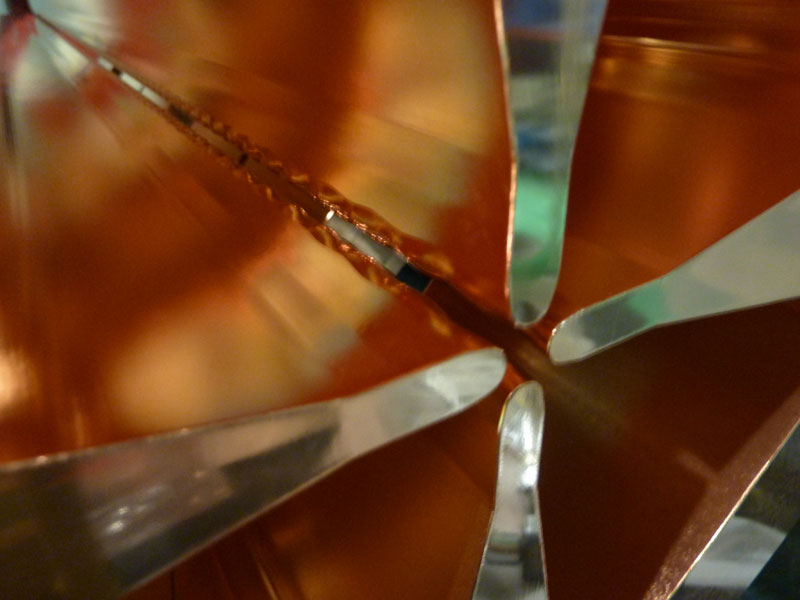
\includegraphics[width=\textwidth]{Figures/LHC_Diagrams/LHC__Linac2__RFQ.jpg}
        \caption{A close-up image of a RFQ, showing the precise
          machining of the longitudanal modulation of the flanges}\label{fig:rfq_actual}
      \end{subfigure}
      ~ %add desired spacing between images, e. g. ~, \quad, \qquad, \hfill etc.
      % (or a blank line to force the subfigure onto a new line)
      \begin{subfigure}[h]{0.4\textwidth}
        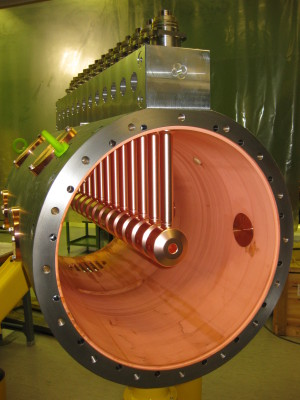
\includegraphics[width=\textwidth]{Figures/LHC_Diagrams/LHC__Linac2__AlvarezTube_Inside__DTL_proto_assembled_image.jpg}
        \caption{The inside of an Alveraz tank, showing the central
          drift tubes, where the protons are accelerated at each gap
          between successive drift tubes}\label{fig:alvarez_tank_inside}
      \end{subfigure}
      ~ %add desired spacing between images, e. g. ~, \quad, \qquad, \hfill etc.
      % (or a blank line to force the subfigure onto a new line)
      \begin{subfigure}[h]{0.4\textwidth}
        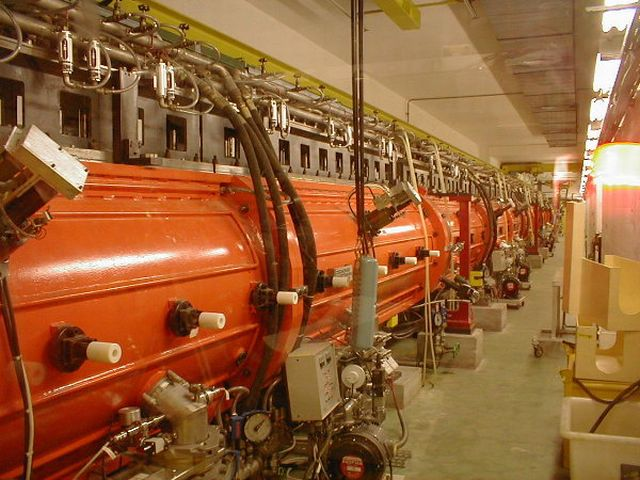
\includegraphics[width=\textwidth]{Figures/LHC_Diagrams/LHC__Linac2__AlvarezTubes.jpg}
        \caption{The Alvarez tanks at the Linac2}\label{fig:alvarez_tank_actual}
      \end{subfigure}
      \caption{Features of the Linac2, the first stage of
        acceleration in the LHC injection chain} \label{fig:linac2}
\end{figure}

\par Protons are initially accelerated by the Linac2 linear accelator
up to 50
\MeV~\cite{LHC:TDR_Vol3_InjectionChain_Benedikt}~\cite{LHC:LHIC_linac2_lhcTests_Hill}.
A bottle of Hydrogren is attached to a duoplasmatron source.  This
device ionizes the Hydrogren, and creates a 300 mA beam of protons,
through a high-voltage anode, and a geometry designed to focus and
collimate the beam as it leaves the device.  Figure
\ref{fig:linac2}(\subref{fig:duoplasmatron_schematic}) shows a
schematic for this device, showing the gas input on the left, and
proton beam leaving to the right.  Figure
\ref{fig:linac2}(\subref{fig:duoplasmatron_actual}) shows the actual
device used in the Linac2 at CERN.  The proton beam then enters the
Radio-Frequency Quadropole (RFQ) system, which accelerates and bunches
the protons up to 750 keV.  The RFQ is a waveguide with four flanges,
which have been machined with a sinusoidal modulation in the
longitudanal direction, which creates an standing electric wave in
this direction, accelerating the protons.  Figure
\ref{fig:linac2}(\subref{fig:rfq_schematic}) shows a schematic of this
modulation, and figure \ref{fig:linac2}(\subref{fig:rfq_actual}) is a
close-up image of this modulation in an actual RFQ. The last stage of
acceleration is provided by three Alvarez tanks.  Each Alvarez tank
holds a series of elctrically isolated cylinders, known as drift
tubes, coaxial with the main tank, with gaps in between them. An
alternating electric field is present in the gaps, and space between
each drift tube and the walls of the tank.  Protons passing through
the center of the drift tubes feel no electric field, but the gaps are
located such that, a proton will always see an accelerating field in
the gap, and are thus receive a boost of energy from each gap as it
traverses the length of the three tanks.  Figure
\ref{fig:linac2}(\subref{fig:alvarez_tank_inside}) shows an image of
the inside of an Alvaez tank, and figure
\ref{fig:linac2}(\subref{fig:alvarez_tank_actual}) shows the tanks at
the Linac2 at CERN.  The final product is a 180 mA, 50 \MeV proton
beam, which is steered to the Proton Synchrotron Booster for the next
stage of acceleration.

\begin{figure}{h}
    \centering
    \begin{subfigure}[h]{0.4\textwidth}
        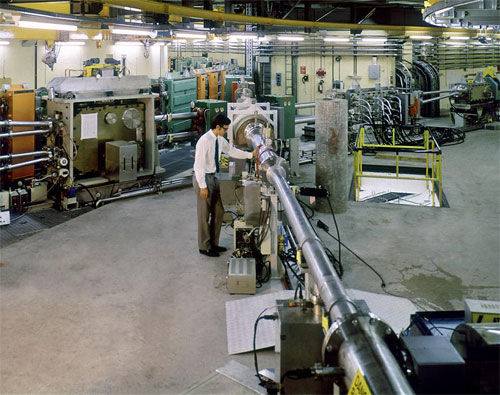
\includegraphics[width=\textwidth]{Figures/LHC_Diagrams/LHC__PSbooster__psb_injection.jpg}
        \caption{The Injection site from the Linac2 into the PS booter}\label{fig:linac2_to_psbooster_injection}
      \end{subfigure}
      ~ %add desired spacing between images, e. g. ~, \quad, \qquad, \hfill etc.
      % (or a blank line to force the subfigure onto a new line)
      \begin{subfigure}[h]{0.4\textwidth}
        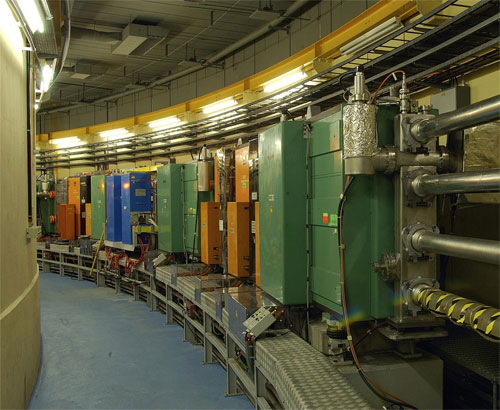
\includegraphics[width=\textwidth]{Figures/LHC_Diagrams/LHC__PSbooster__psb_4_beamLines_shown.jpg}
        \caption{A section of the PS booster, with the four stack
          synchotron beamlines shown in the lower right hand side of the picture}\label{fig:psbooster_4stacks}
      \end{subfigure}
       ~ %add desired spacing between images, e. g. ~, \quad, \qquad, \hfill etc.
      % (or a blank line to force the subfigure onto a new line)
      \begin{subfigure}[h]{0.4\textwidth}
        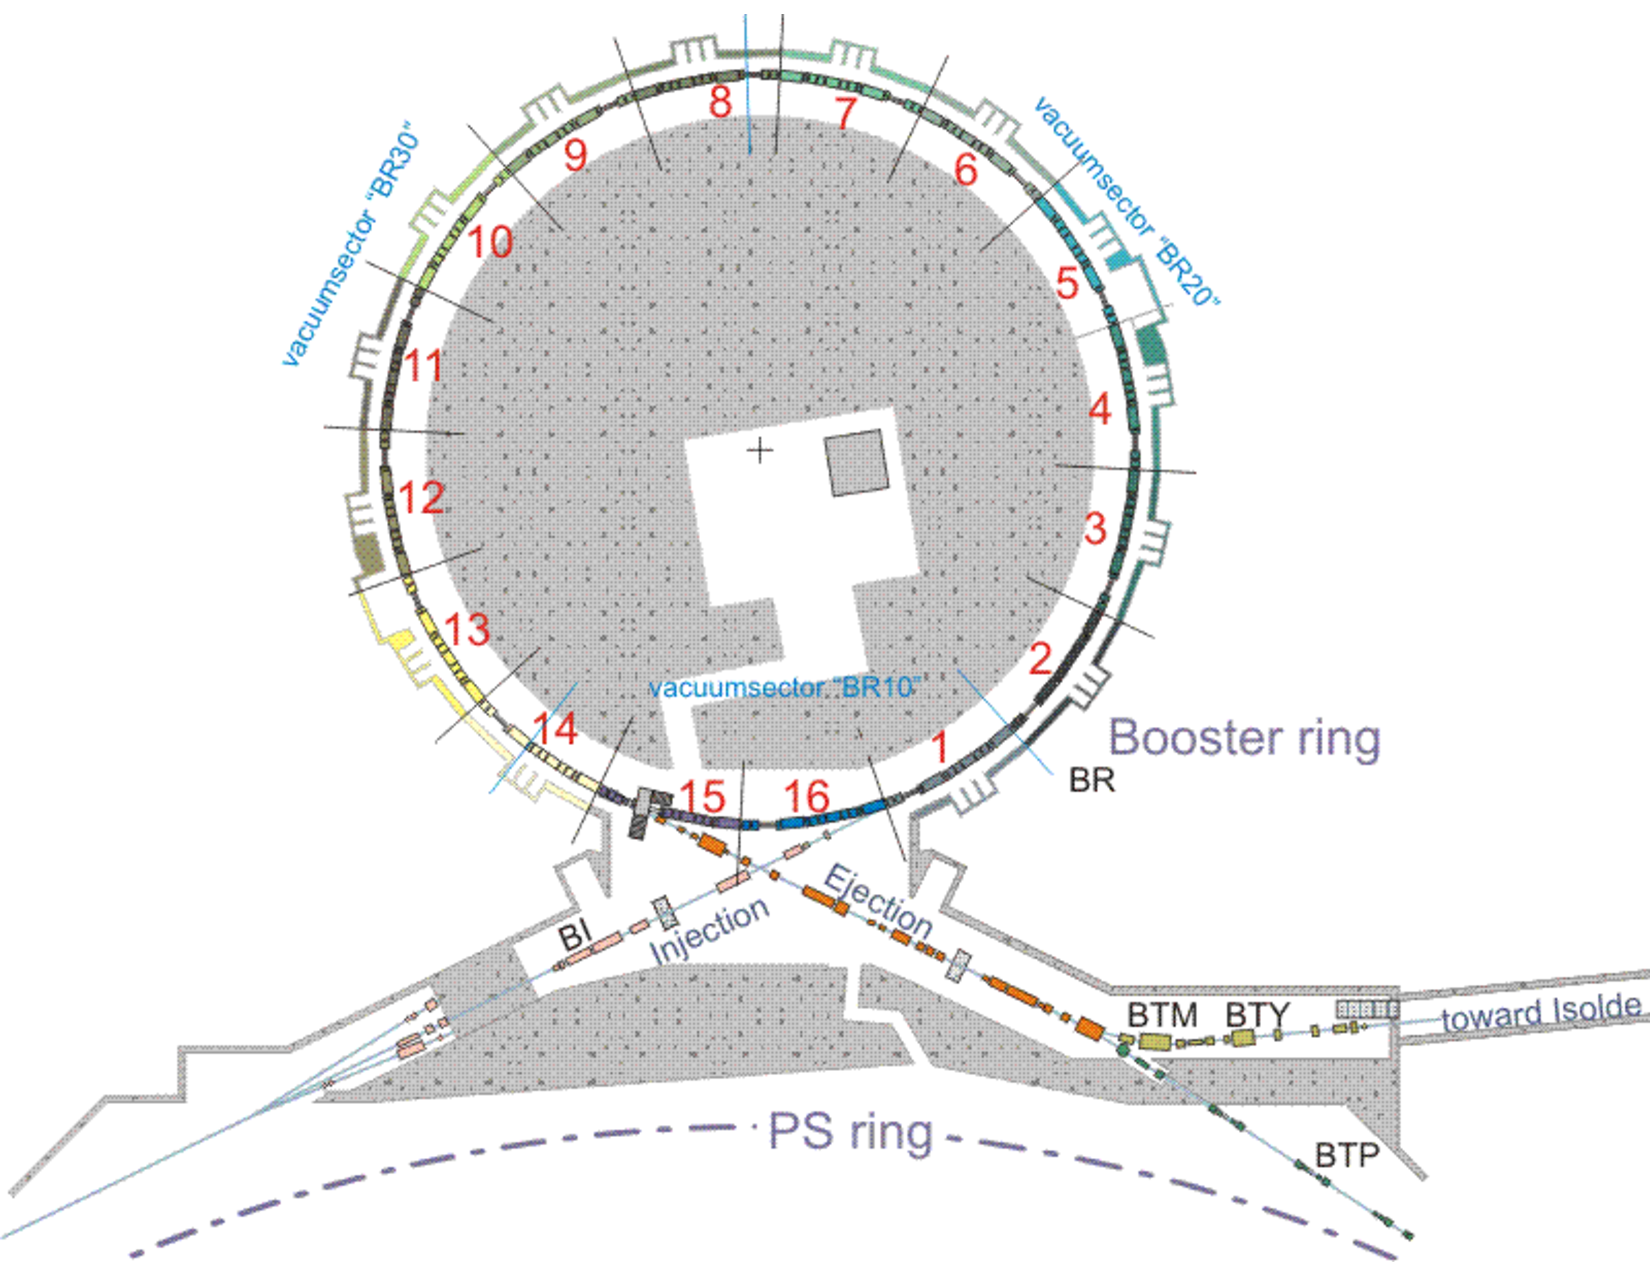
\includegraphics[width=\textwidth]{Figures/LHC_Diagrams/LHC__PSbooster__Layout.pdf}
        \caption{A drawing of the 16 sections of the PS booster}\label{fig:psbooster_16sections}
      \end{subfigure}
       ~ %add desired spacing between images, e. g. ~, \quad, \qquad, \hfill etc.
      % (or a blank line to force the subfigure onto a new line)
      \begin{subfigure}[h]{0.4\textwidth}
        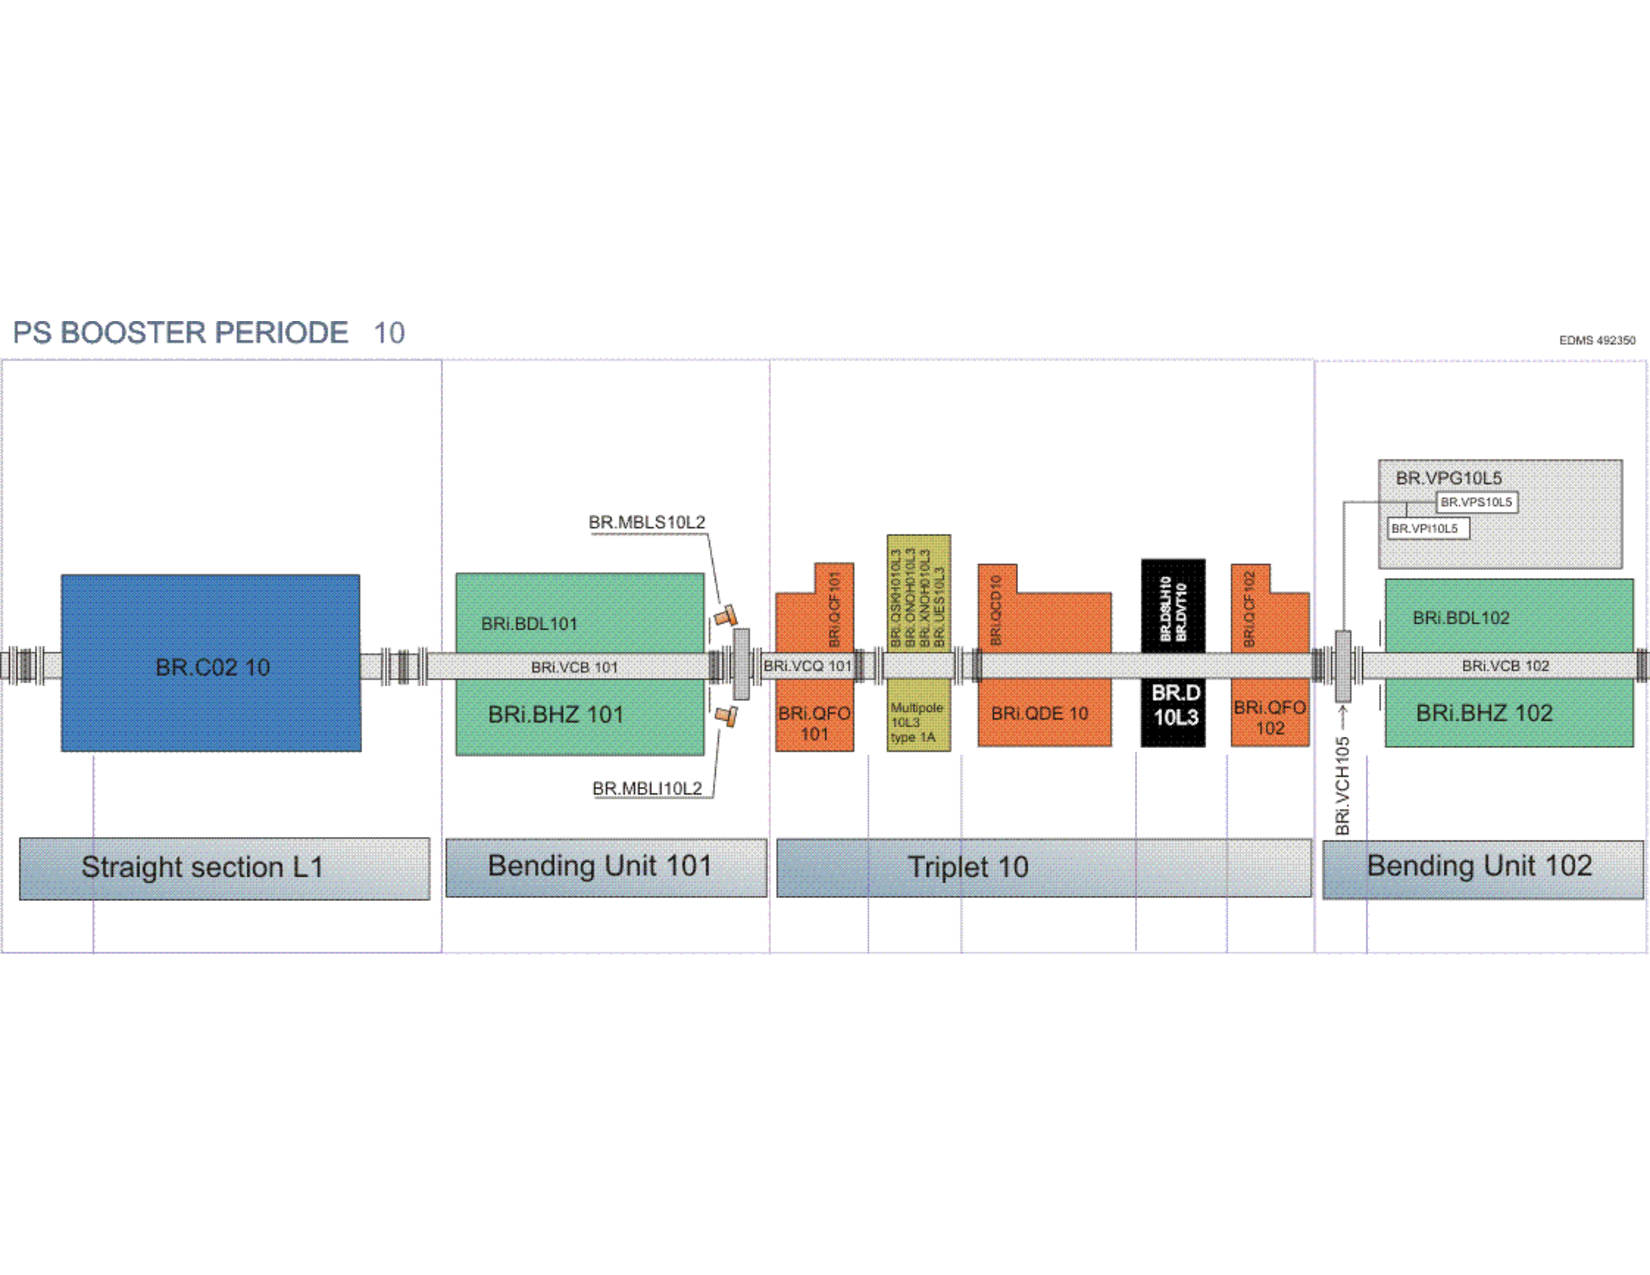
\includegraphics[width=\textwidth]{Figures/LHC_Diagrams/LHC__PSbooster__sect10.pdf}
        \caption{Section 10 of the PS booster.  This begins with the
          CO2 cavity, the main driver of the acceleration; followed by
        a dipole magnet, a triplet of focusing magnets, and a second
        dipole magnet}\label{fig:psbooster_section10}
      \end{subfigure}
      ~ %add desired spacing between images, e. g. ~, \quad, \qquad, \hfill etc.
      % (or a blank line to force the subfigure onto a new line)
      \begin{subfigure}[h]{0.4\textwidth}
        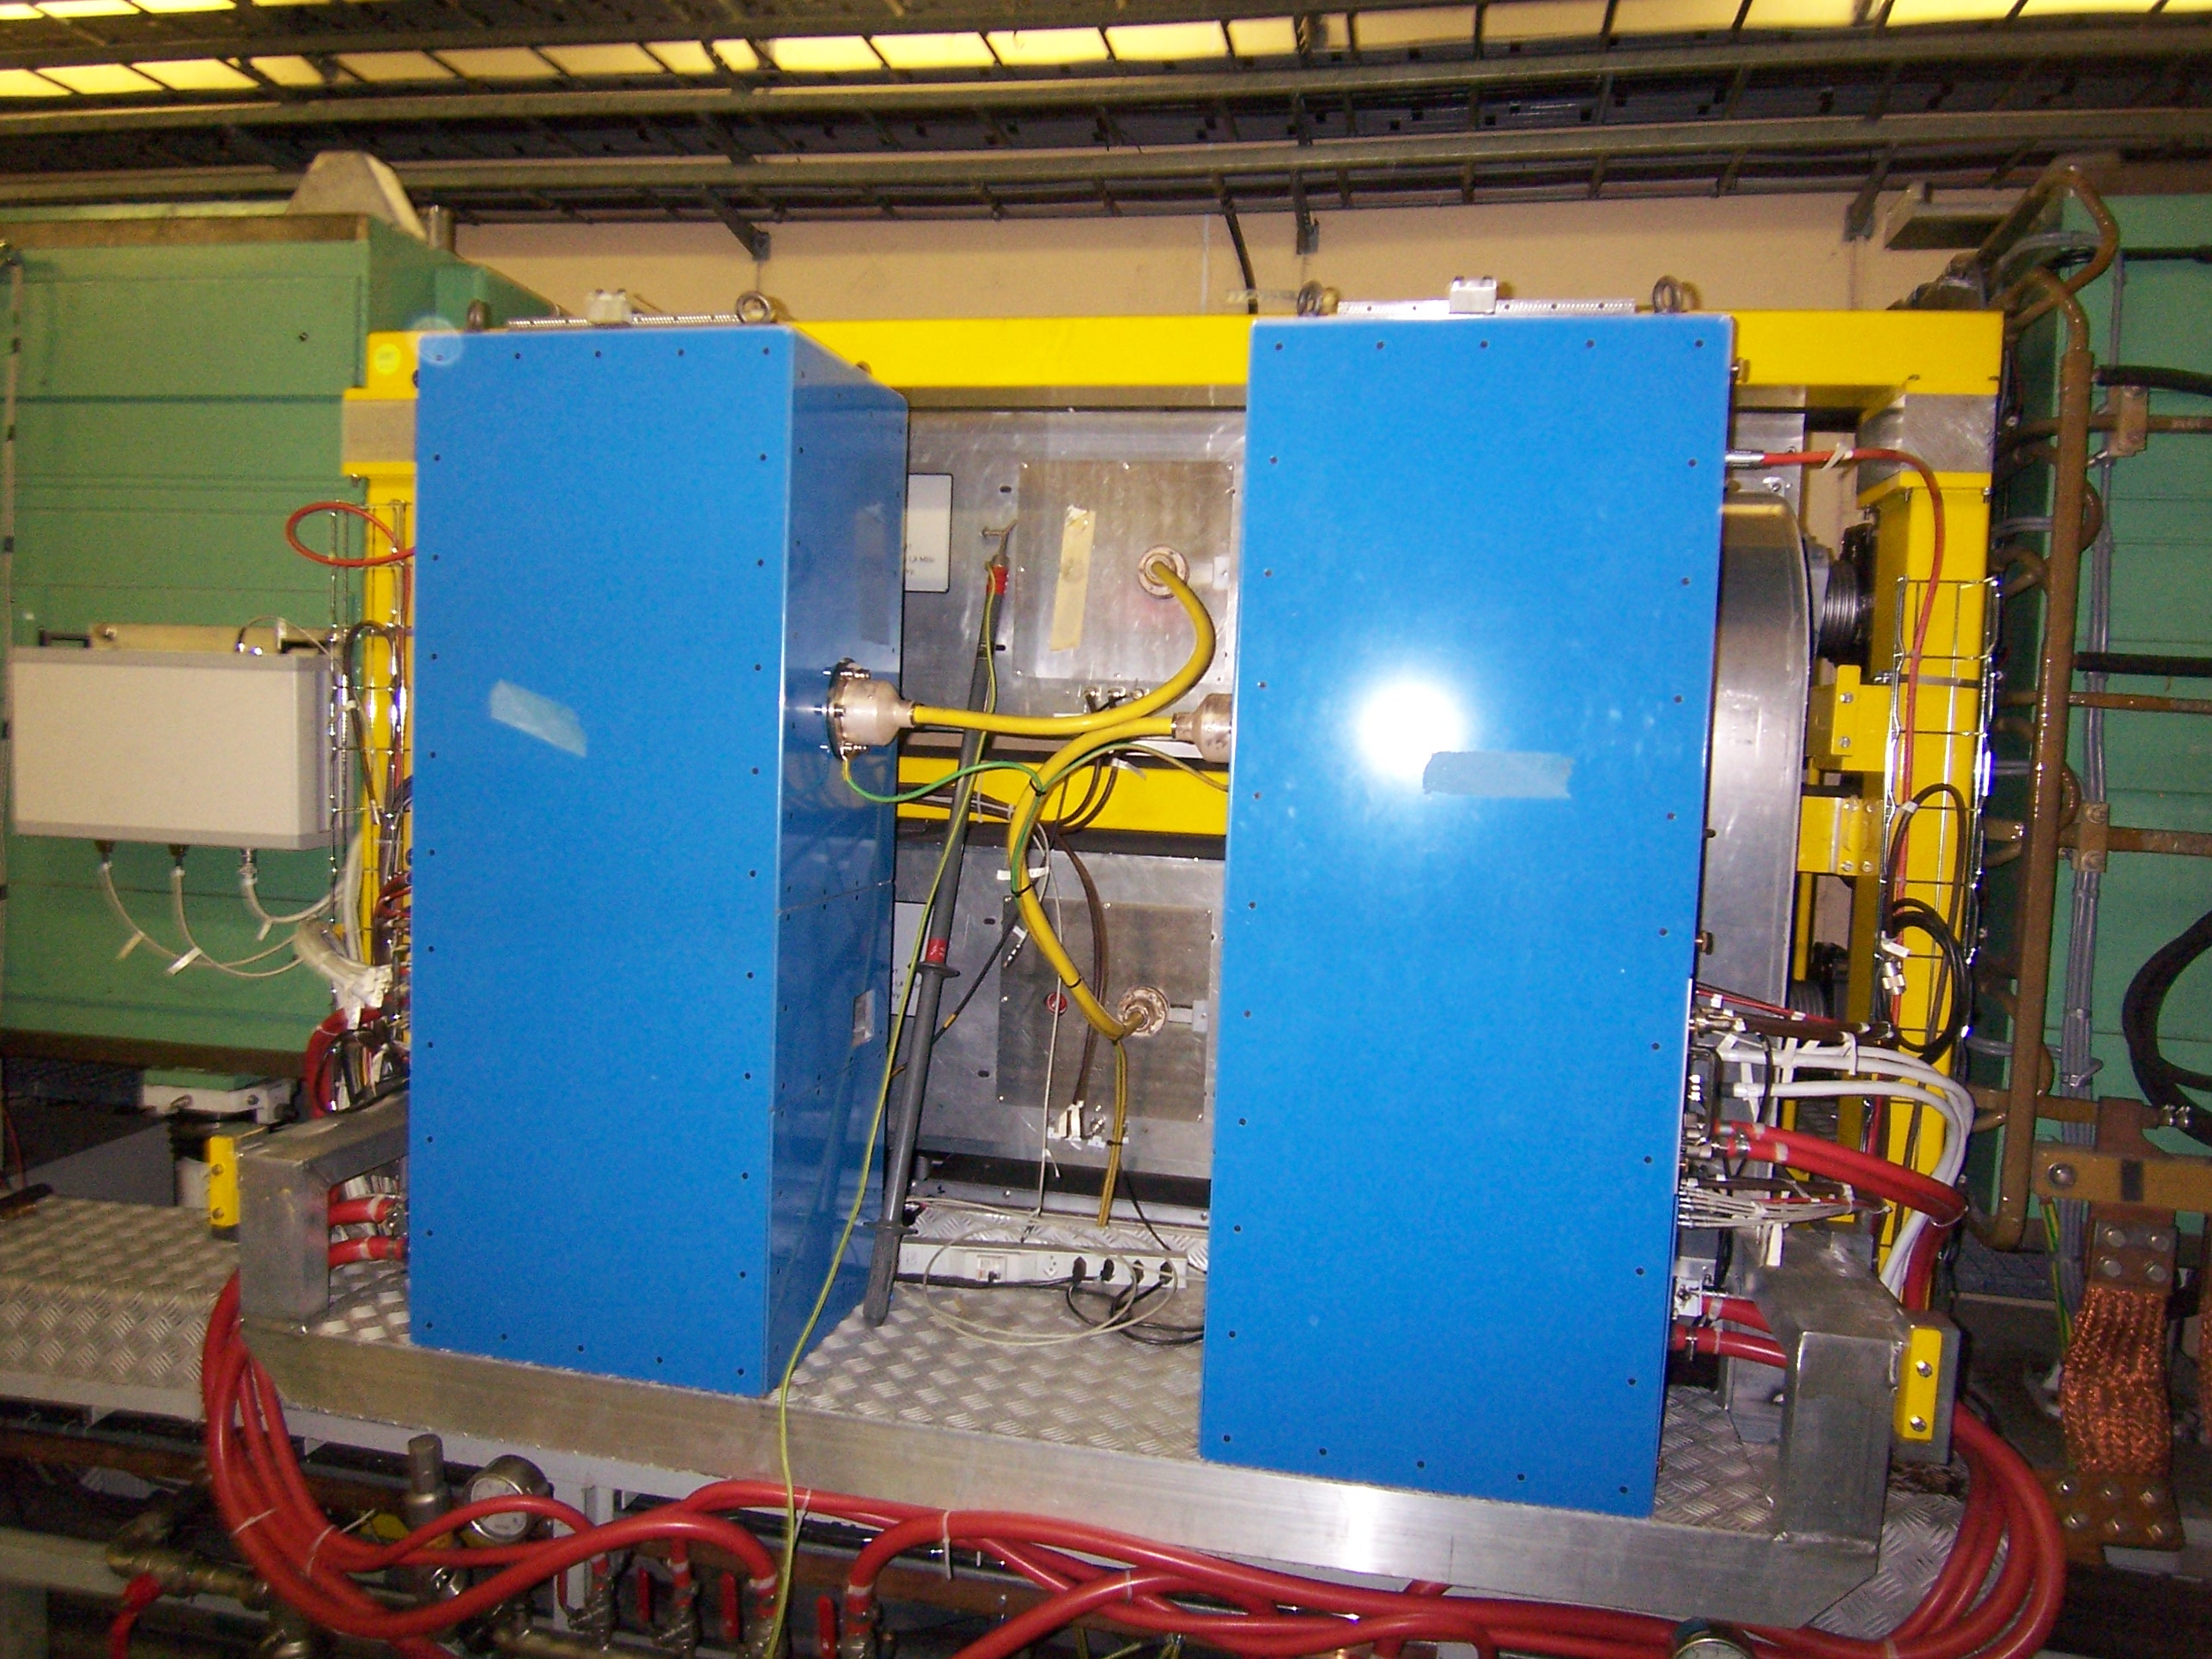
\includegraphics[width=\textwidth]{Figures/LHC_Diagrams/LHC__PSbooster__CO2_RFCavity__P10L1.JPG}
        \caption{A picture of the CO2 RF Cavity, which provides the
          priniciple acceleration for the protons in the PS booster}\label{fig:psbooster_CO2_RFCavity}
      \end{subfigure}
      ~ %add desired spacing between images, e. g. ~, \quad, \qquad, \hfill etc.
      % (or a blank line to force the subfigure onto a new line)
      \begin{subfigure}[h]{0.4\textwidth}
        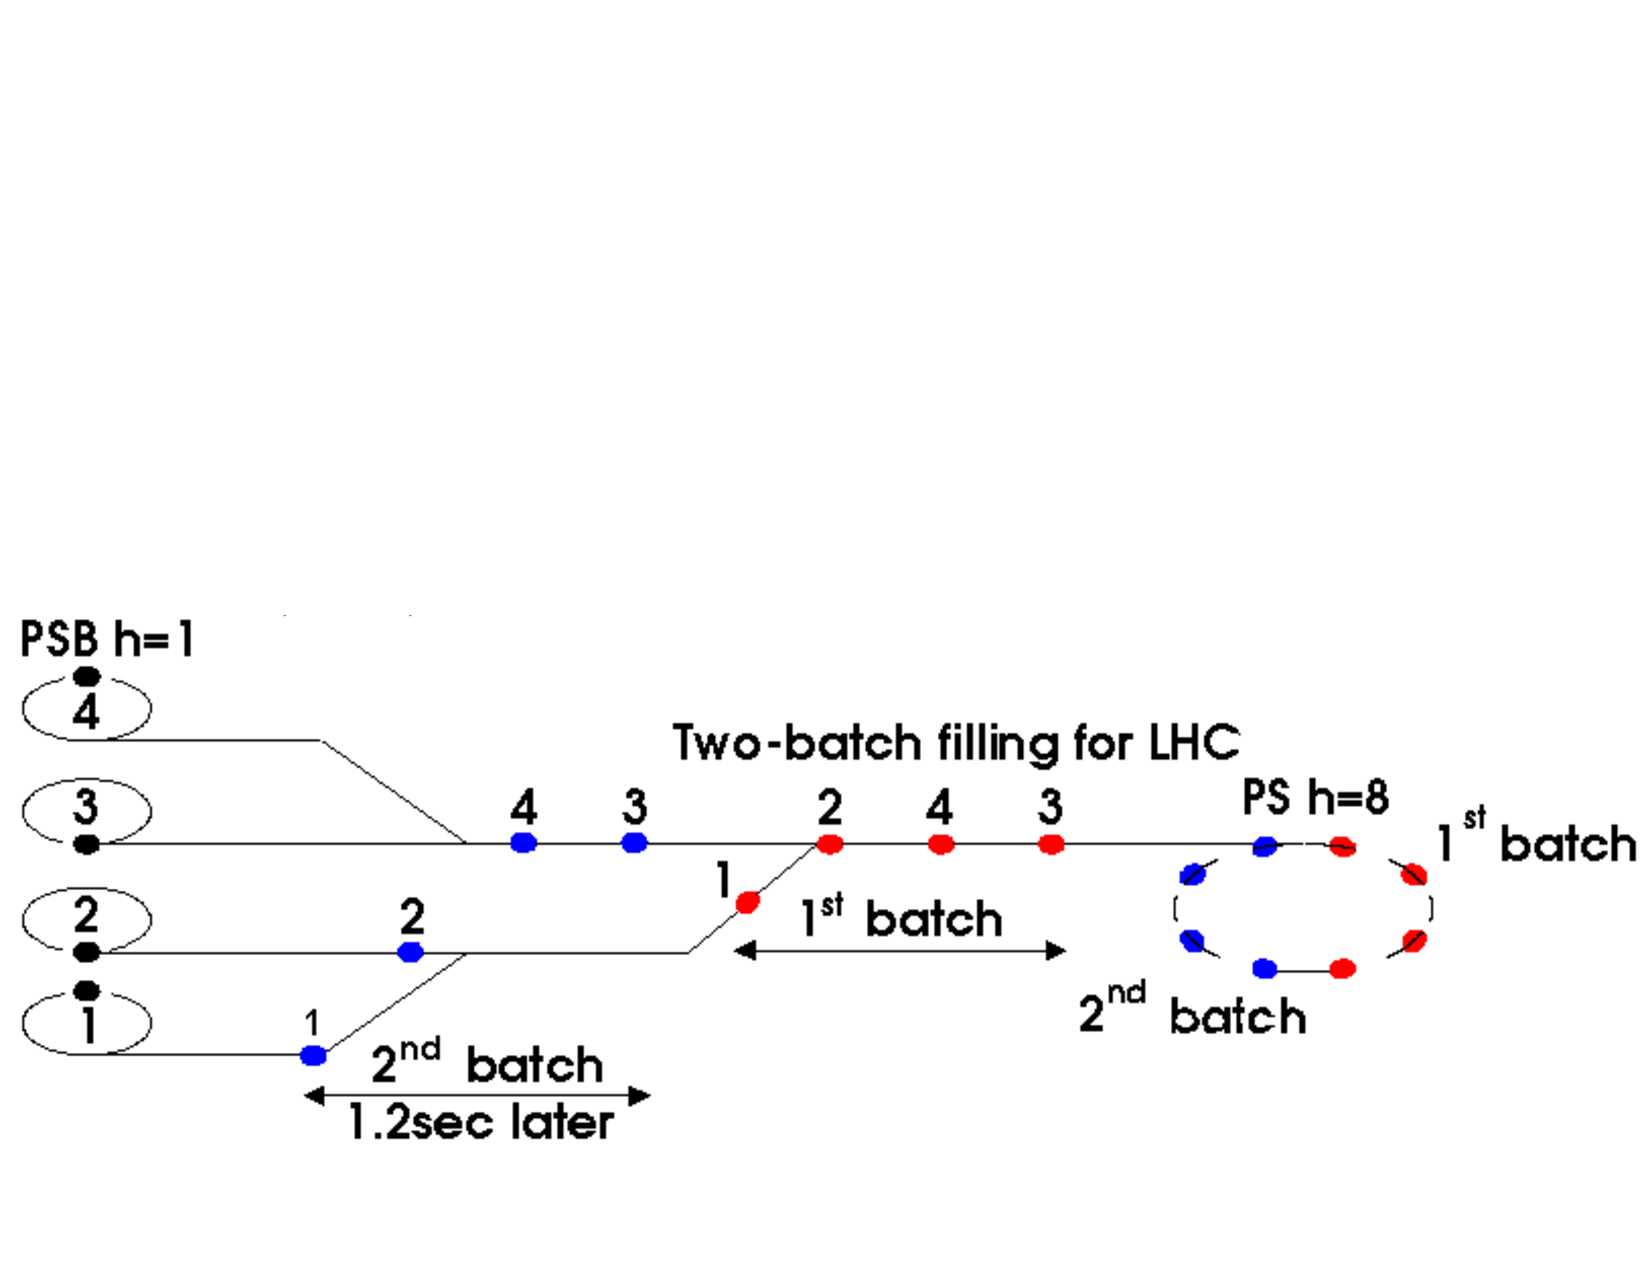
\includegraphics[width=\textwidth]{Figures/LHC_Diagrams/LHC__PSbooster__2batchFillingScheme__schindlrf.pdf}
        \caption{The two batch filling scheme for the PS.  It takes
          1.2 s for each batch to be accelerated from 50 \MeV to 1.4 \GeV}\label{fig:psbooster_2batchScheme}
      \end{subfigure}
      \caption{Features of the PS booster, the second stage of
        the LHC injection chain}\label{fig:psbooster}
\end{figure}

\par The Proton Synchotron Booster (PS booster) complex accelerates
the protons up to 1.4
\GeV~\cite{LHC:TDR_Vol3_InjectionChain_Benedikt}.  The complex takes
the proton beam from the Linac2 and splits the beam into four
separate, synchrotrons, stacked on top of one another.  Figure
\ref{fig:psbooster}(\subref{fig:linac2_to_psbooster_injection}) shows the
injection site of the proton beam from the Linac2 into the PS booter.
The right side of figure
\ref{fig:psbooster}(\subref{fig:psbooster_4stacks}) shows the four
synchotron beam pipes stacked vertically on top one another.  The
splitting of the beam is done in order to reduce the effect of the
space charge of the proton beam, which would increase the transverse
emmitance beyond a tolerable degree.  The PS booster uses thirty-two
0.87 T dipole magnets to bend the beams, and fourty-eight quadrupoles
to focus the beam as it makes its way around each of the 50 m diameter
rings.  Each magnet is composed of a vertical stack of four magnets,
one for each of the synchotrons, and share a common yoke, allowing one
power supply to provide the current to all of them in 
series~\cite{LHC:LHC_psbooster_boosterTurns40}.  The booster is
divided into 16 arcs, as shown in figure
\ref{fig:psbooster}(\subref{fig:psbooster_16sections}).  Each arc contains
a bending dipole, 3 focusing quadrupoles, and a second bending dipole,
followed by a straight section containing beam diagnostic, injection
and ejection systems, and in three sections, the Radio-Frequency (RF) cavities, which is
the mechanism of accelerating the
beam~\cite{LHC:LHC_psbooster_layout}.  Figure
\ref{fig:psbooster}(\subref{fig:psbooster_section10}) shows the layout
of the tenth arc, which also contains one of the RF cavities in the first
section.
  
\par An RF cavity is a specially shaped, hollow
conductor, that the beam passes
through~\cite{LHC:BasicsOfAccelerators_Baird}.  The shape of the
cavity determines the resonant frequency and harmonics (integer
multiples of the fundamental frequency), of the standing
electromagnetic fields that result when the cavity is driven by an
alternating voltage source.  The idea is to choose a resanant
frequency such that the proton will always experience a positive
electric field, and thus an acceleration, each time it passes through
the RF cavity.  This means that the revolution requency of the proton
must be equal to the fundamental frequency or harmonic of the RF
cavity, $f_{RF} = n{\times}f_{rev}$, with $n=1,2,3...$.  Eventually,
the proton is accelerated up to an equilibrium speed and will enter the
cavity just as the standing electric field is alternating through it's
zero point.  If arrives too early for this (moving too fast), then it
will experience a negative electric force, a decceleration, which will
eventually bring it back to the equilibrium revolution frequency,
where it experiences zero net force.  A diffuse beam of protons will
be bunched into groups of protons through this effect as well, as the
faster protons in the beams are deccelerated, and the slower ones
accelerated, until they all reach the same equilibrium revolution
frequency.  Driving  the RF cavity with a harmonic, n, of the proton's
revolution speed will thus create n bunches of protons.  Each one of
the potential n bunch positions is referred to as a bucket.  In the
case where a proton has to be accelerated through a wide range of
energies, the frequency of the cavity must also increase to maintain
synchronization with the proton revolution frequency.  

\par Three types of RF cavities are used to accelerate the beam
during each revolution.  The first of the three types of RF cavities
is the CO2, with frequency range of 0.6 to 2.0 MHz and is used to
drive the $h=1$ harmonic of the  synchrotron, and is pictured in
figure \ref{fig:psbooster}(\subref{fig:psbooster_CO2_RFCavity}).  The
second type of cavity is the CO4 chamber, with a frequency range of
1.2 to 3.9 MHz, and drives the $h=2$ mode of the synchrotron.  This
second mode is capable of spliting the beam and creating two separate
bunch  structures.  However, for LHC running, only one bunch is used,
and is driven primarily by the $h=1$ mode.  The $h=2$ mode is
supplemental and is used to shape the beam.  A third type of RF
cavity, CO16, has a frequency range of 5 to 16 MHz, and is used to
control the longitudal shape of a bunch during acceleration. The beam
leaves the PS booster and enters the PS in a two-batch filling scheme,
taking only 1.2 s to accelerate a second batch of protons from 50 \MeV
to 1.4 \GeV.  This second batch enters just as the first batch has
traveled to the opposite side of the PS ring.  A schematic of this
process is shown in figure
\ref{fig:psbooster}(\subref{fig:psbooster_2batchScheme}).  To acheive
the 25 ns bunch spacing design of the LHC, only 6 bunches of proton
beam need to be delivered to PS.  This is acheived by either using a
4+2 or 3+3 filling scheme, in terms of the number of proton bunches
delived from the four possible synchotrons.   

\begin{figure}{h}
    \centering
    \begin{subfigure}[h]{0.45\textwidth}
        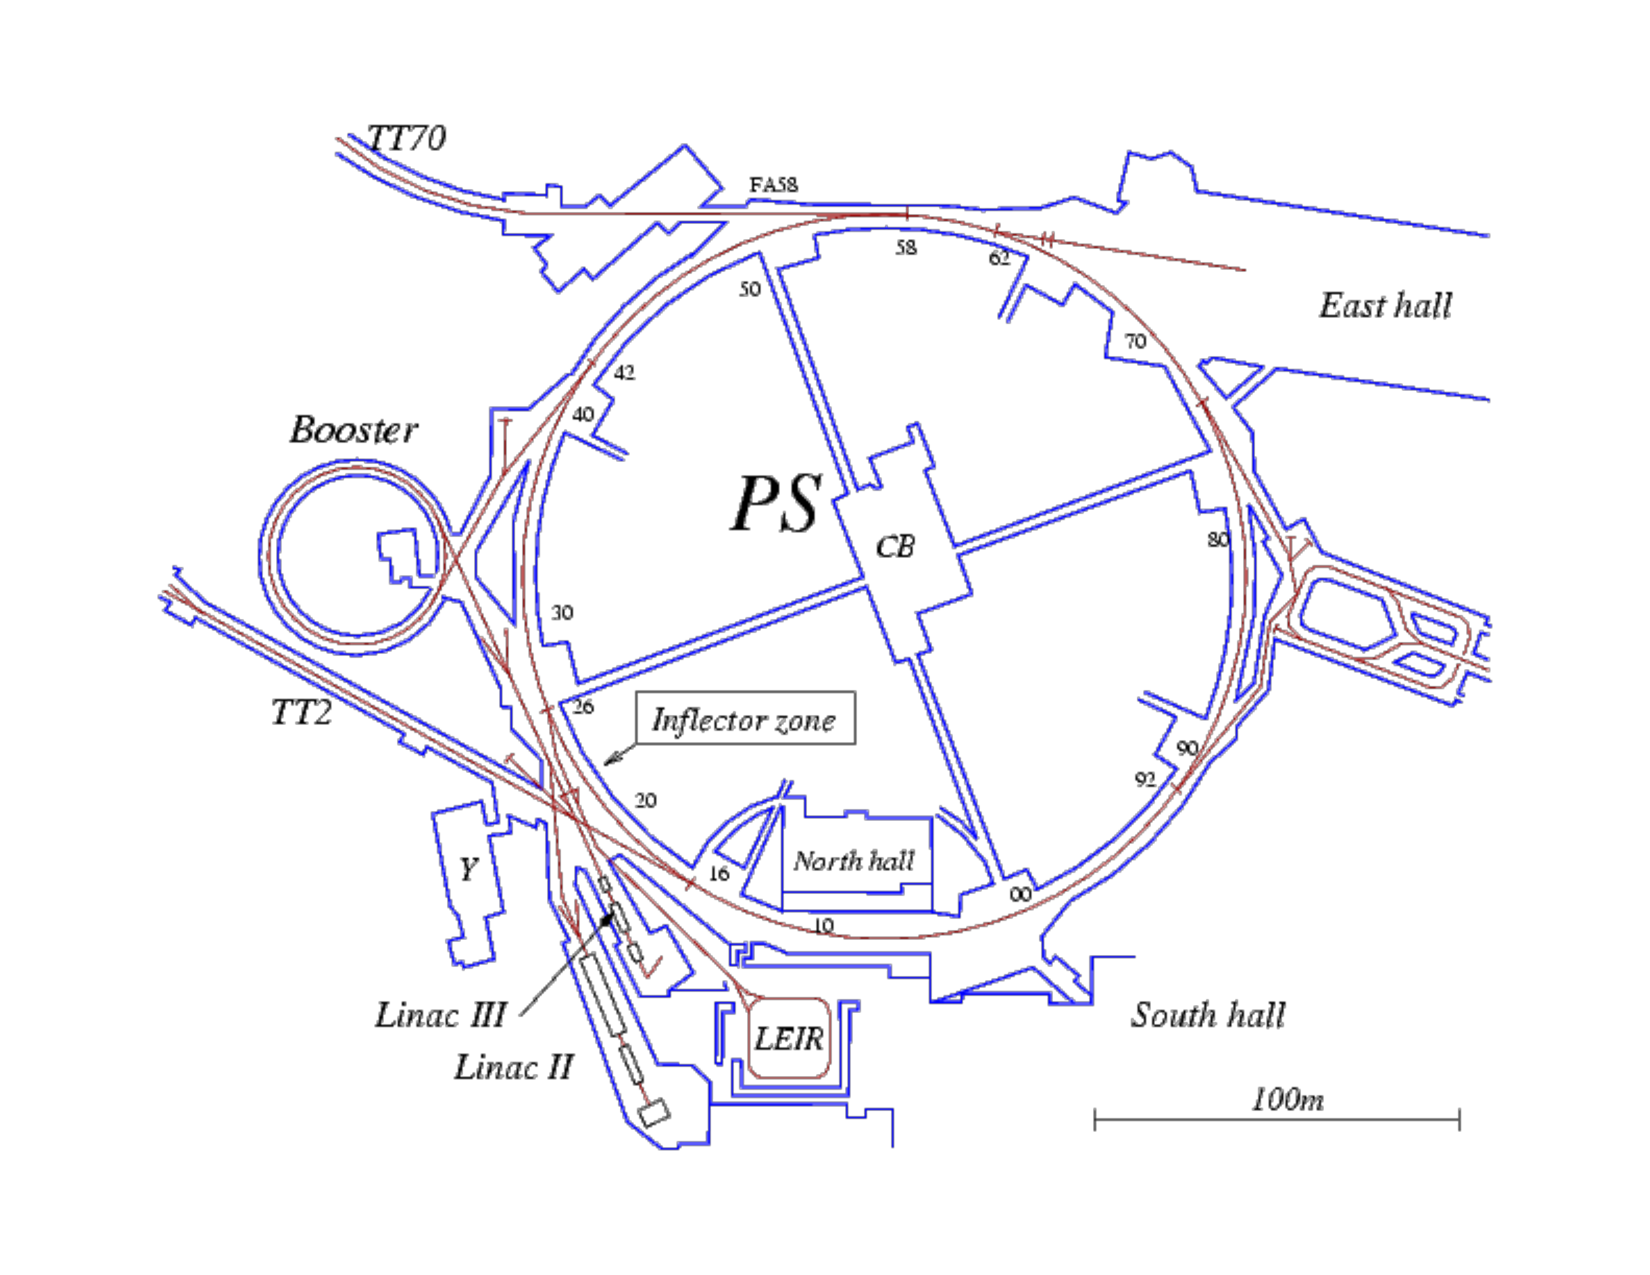
\includegraphics[width=\textwidth]{Figures/LHC_Diagrams/LHC__PS__pscomplex.pdf}
        \caption{A diagram of the PS layout}\label{fig:ps_layout}
      \end{subfigure}
      ~ %add desired spacing between images, e. g. ~, \quad, \qquad, \hfill etc.
      % (or a blank line to force the subfigure onto a new line)
    \begin{subfigure}[h]{0.45\textwidth}
        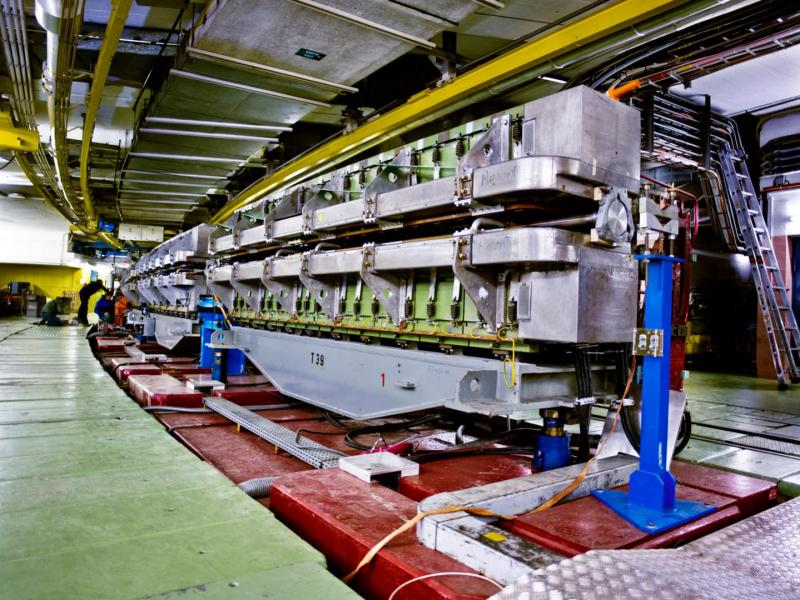
\includegraphics[width=\textwidth]{Figures/LHC_Diagrams/LHC__PS__Dipoles_accelerators-ps.jpg}
        \caption{Dipole magnets used to steer the beam around the 100
          m radius PS ring}\label{fig:ps_dipoles}
      \end{subfigure}
      ~ %add desired spacing between images, e. g. ~, \quad, \qquad, \hfill etc.
      % (or a blank line to force the subfigure onto a new line)
      \begin{subfigure}[h]{0.45\textwidth}
        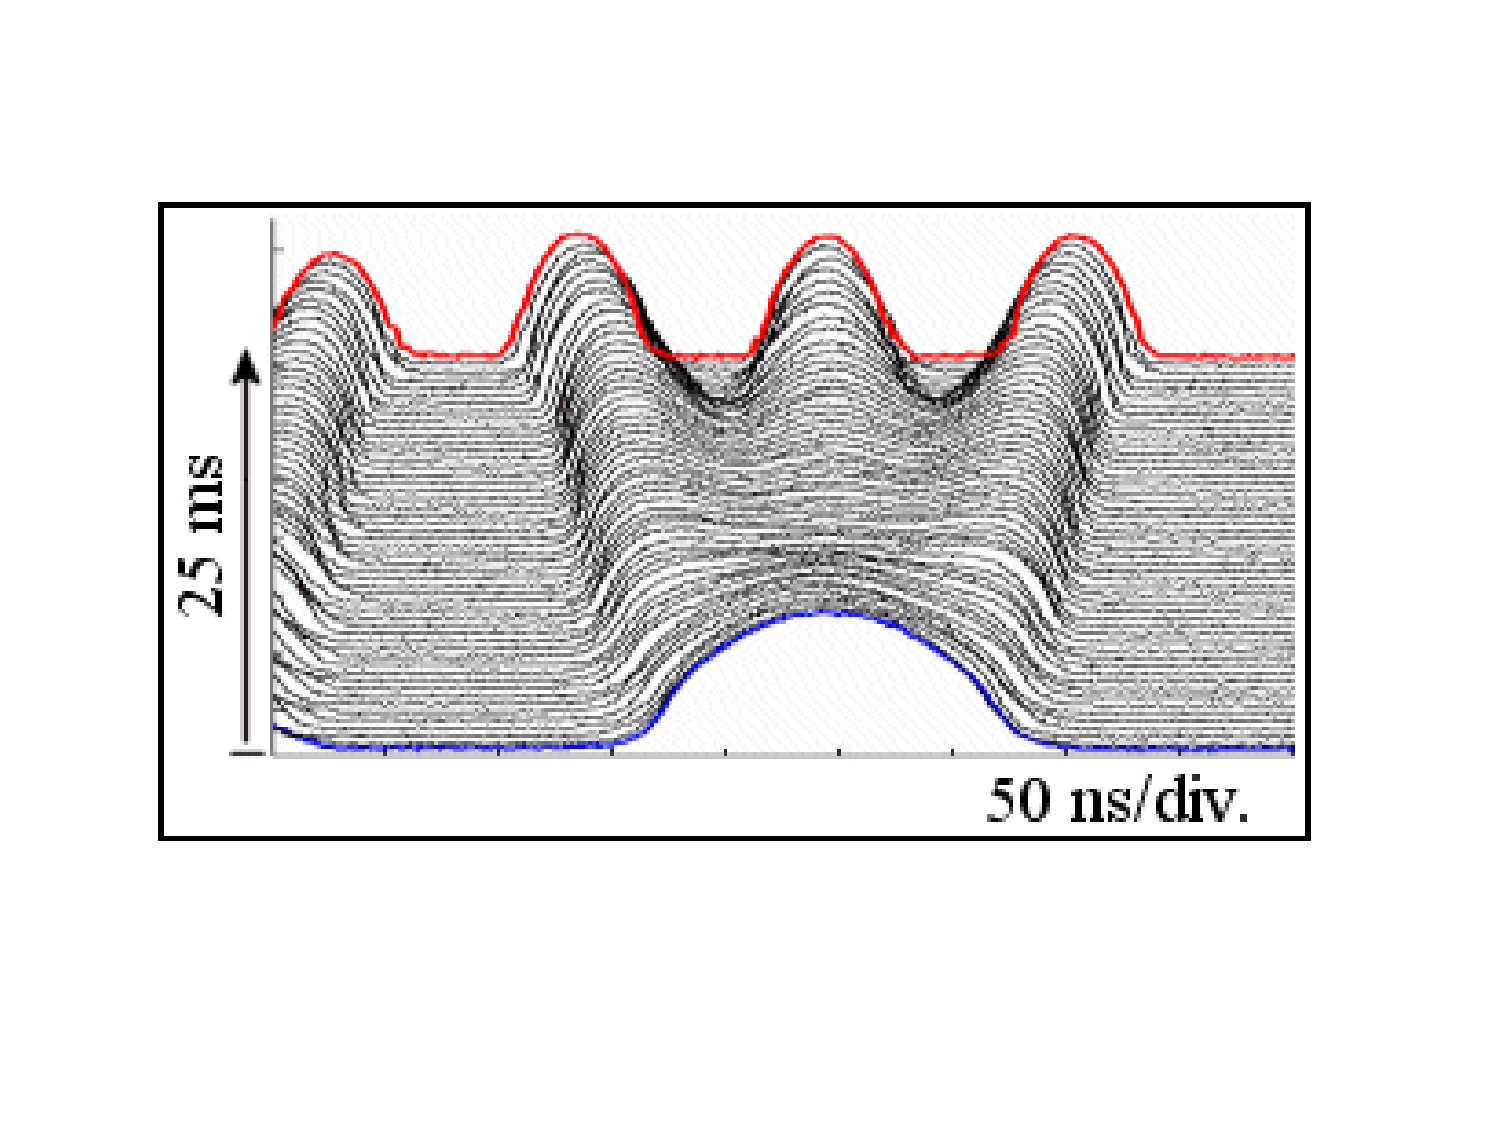
\includegraphics[width=\textwidth]{Figures/LHC_Diagrams/LHC__PS__TripleBunchSplitting.pdf}
        \caption{A simulation of the PS using the $h=7,14,21$ modes of
        to split the beam into 3 bunches}\label{fig:ps_split3}
      \end{subfigure}
       ~ %add desired spacing between images, e. g. ~, \quad, \qquad, \hfill etc.
      % (or a blank line to force the subfigure onto a new line)
      \begin{subfigure}[h]{0.45\textwidth}
        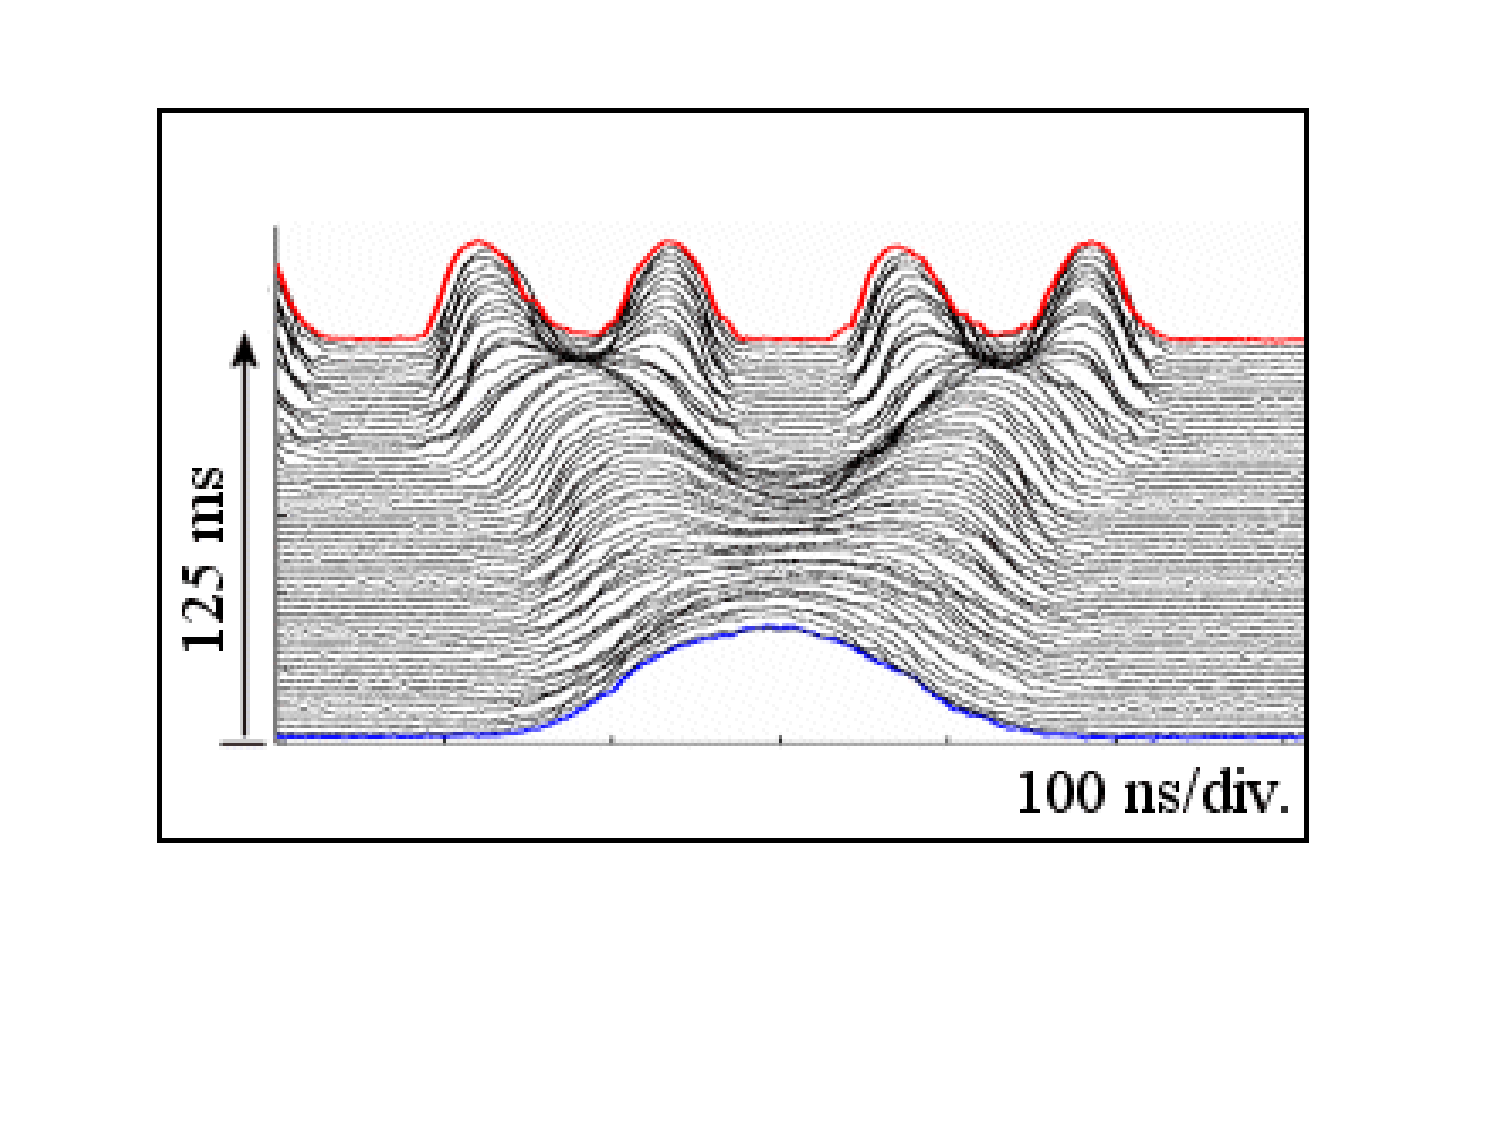
\includegraphics[width=\textwidth]{Figures/LHC_Diagrams/LHC__PS__DoubleDoubleBunchSplitting.pdf}
        \caption{A simulation of the }\label{fig:ps_split2x2}
      \end{subfigure}
       ~ %add desired spacing between images, e. g. ~, \quad, \qquad, \hfill etc.
      % (or a blank line to force the subfigure onto a new line)
      \begin{subfigure}[h]{0.45\textwidth}
        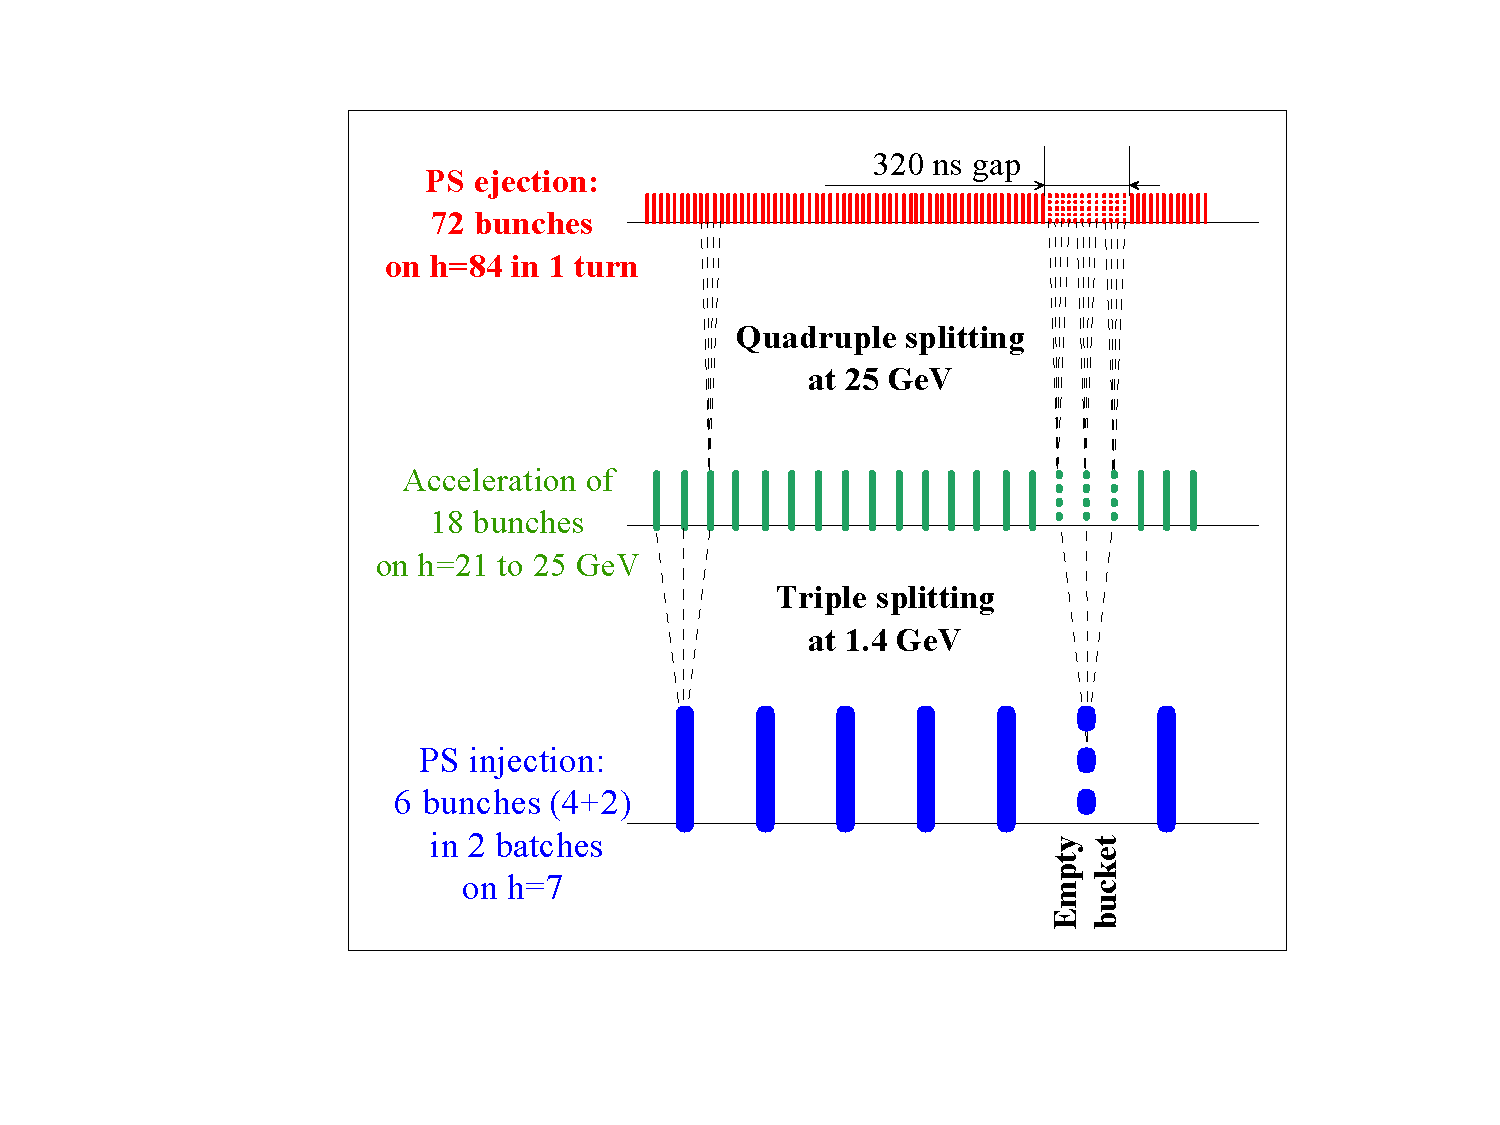
\includegraphics[width=\textwidth]{Figures/LHC_Diagrams/LHC__PS__BunchSplittingDiagram.pdf}
        \caption{An overview of the splitting procedure}\label{fig:ps_splitting}
      \end{subfigure}
      ~ %add desired spacing between images, e. g. ~, \quad, \qquad, \hfill etc.
      % (or a blank line to force the subfigure onto a new line)
      \begin{subfigure}[h]{0.45\textwidth}
        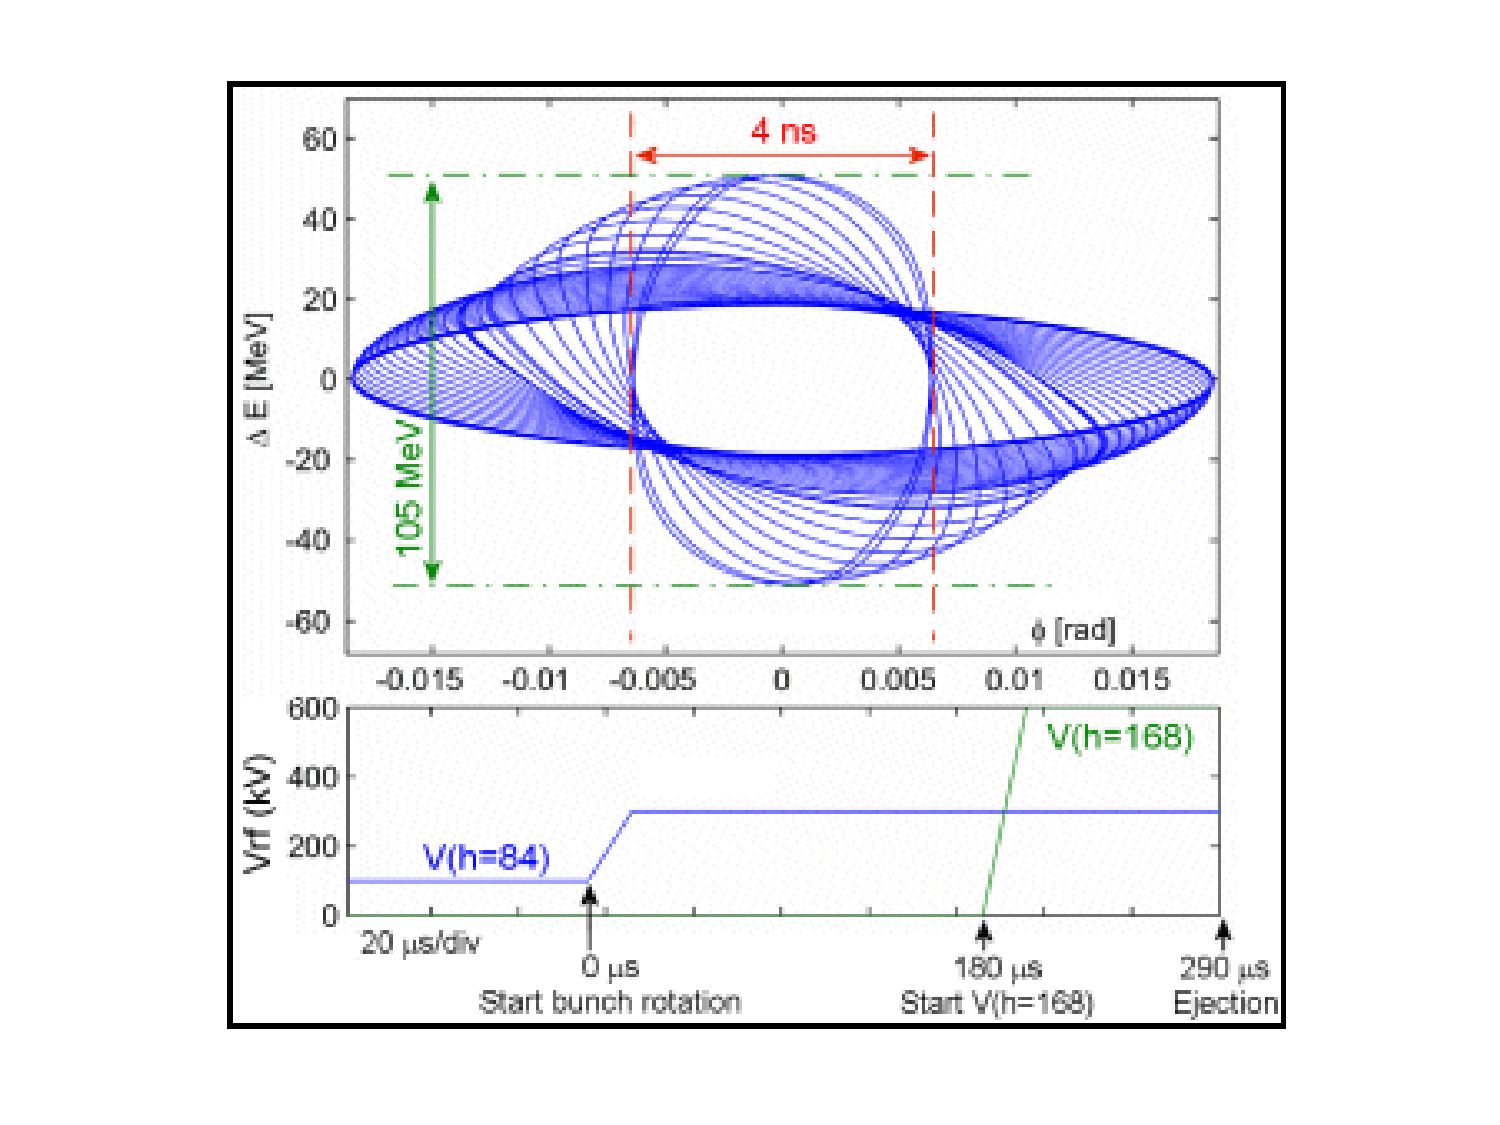
\includegraphics[width=\textwidth]{Figures/LHC_Diagrams/LHC__PS__BunchCompression.pdf}
        \caption{Rotation in phase space of the 25 \GeV proton beam,
          compressing the bunch lengths from 11 ns to 4 ns}\label{fig:ps_bunch_compression}
      \end{subfigure}
      \caption{Features of the PS, the third stage of
        the LHC injection chain}\label{fig:ps}
\end{figure}


\par The next stage is the Proton Synchrotron (PS), which will boost the
protons up to 25 \GeV~\cite{LHC:TDR_Vol3_InjectionChain_Benedikt}.
The layout is shown in figure \ref{fig:ps}(\subref{fig:ps_layout}).  
The ring has a circumfrence of 628 m, and uses 100 dipole magnets and
177 higher-order focusing magnets, to steer the beam around the ring.
Figure \ref{fig:ps}(\subref{fig:ps_dipoles}) shows a picture of one of
the dipole magnets used at the PS.  In addition to providing
acceleration up to 25 \GeV, the PS forms the basis of the bunch
structure that is eventually used in the LHC.  The $h=7$ harmonic is
used to capture the 6 bunches of protons delivered from the PS
booster, leaving a gap in the place of a seventh bunch.  The beam is
then split into three, by using three different RF cavities tuned to
the $h=7,14,21$ modes of the PS.  Figure
\ref{fig:ps}(\subref{fig:ps_split3}) shows a simulation of a proton
bunch being divided  into three over the course of 25 ms.  The $h=21$
mode is then used to accelerate the protons to from 1.4 to 25 \GeV
using the 20 MHz RF cavity.  Each bunch is then split twice,
using the $h=21,42,84$ synchroton modes, to create 72 bunches, spaced
25 ns apart, with a 320 ns gap for the 12 unused buckets of the $h=84$
harmonic. This process is simulated in figure
\ref{fig:ps}(\subref{fig:ps_split2x2}), over the course of 125 ms. The
320 ns gap is created to account for the rise time of the  kicker
magnet, which ejects the beam out of the PS into the SPS.  The entire
splitting process is summarized in figure
\ref{fig:ps}(\subref{fig:ps_splitting}).  For the case of 50 ns bunch
spacing, the final stage of splitting is not performed, and the
$h=21,42$ modes are used to split the beam.  Finally, in order to fit
the bunches into the 200 MHz RF acceleration scheme of the SPS, the 
bunch length must be compressed from 11 ns to 4 ns.  This is acheived
by rotating the beam in the energy vs time phase space by sequential
increases in voltage to the 40 MHz $h=84$ mode, followed by an
increase to the 80 MHz $h=168$ mode.  Figure
\ref{fig:ps}(\subref{fig:ps_bunch_compression}) shows the result of
this rotation - a distortion free ellipse with a smaller 4 ns spread,
but a larger spread in the energy spectrum of the proton beam.   

\begin{figure}{h}
    \centering
    \begin{subfigure}[h]{0.45\textwidth}
        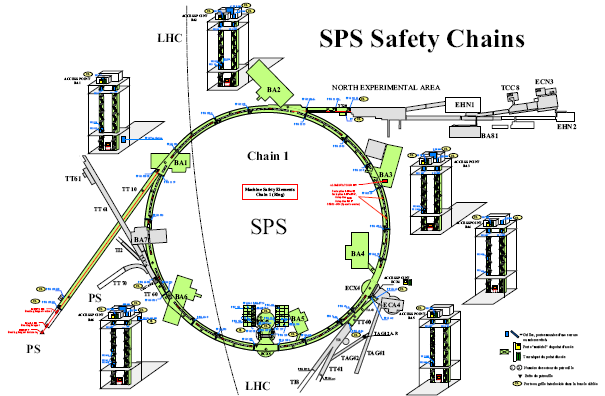
\includegraphics[width=\textwidth]{Figures/LHC_Diagrams/LHC__SPS__layout.png}
        \caption{The layout of the SPS facility}\label{fig:sps_layout}
      \end{subfigure}
      ~ %add desired spacing between images, e. g. ~, \quad, \qquad, \hfill etc.
      % (or a blank line to force the subfigure onto a new line)
    \begin{subfigure}[h]{0.45\textwidth}
        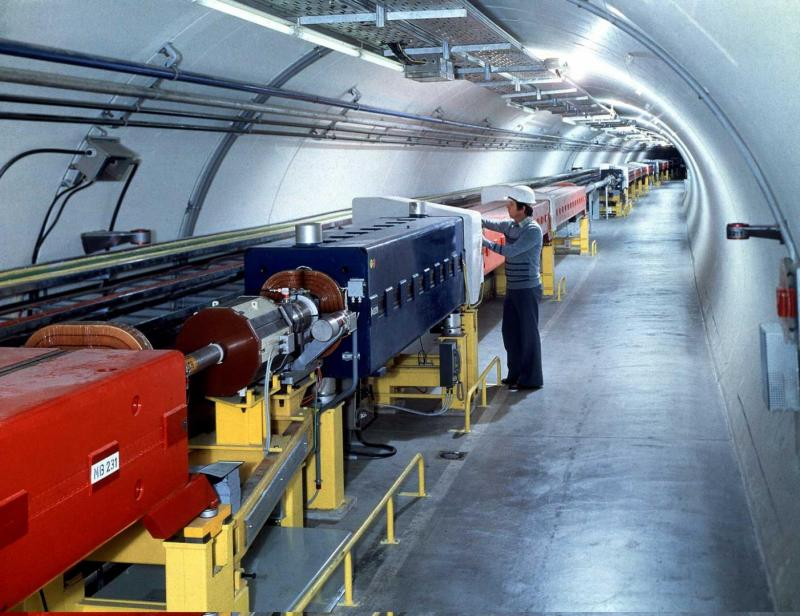
\includegraphics[width=\textwidth]{Figures/LHC_Diagrams/LHC__SPS__beamline.jpg}
        \caption{A sectio of dipole magnets used in the SPS}\label{fig:sps_dipoles}
      \end{subfigure}
      ~ %add desired spacing between images, e. g. ~, \quad, \qquad, \hfill etc.
      % (or a blank line to force the subfigure onto a new line)
      \begin{subfigure}[h]{0.45\textwidth}
        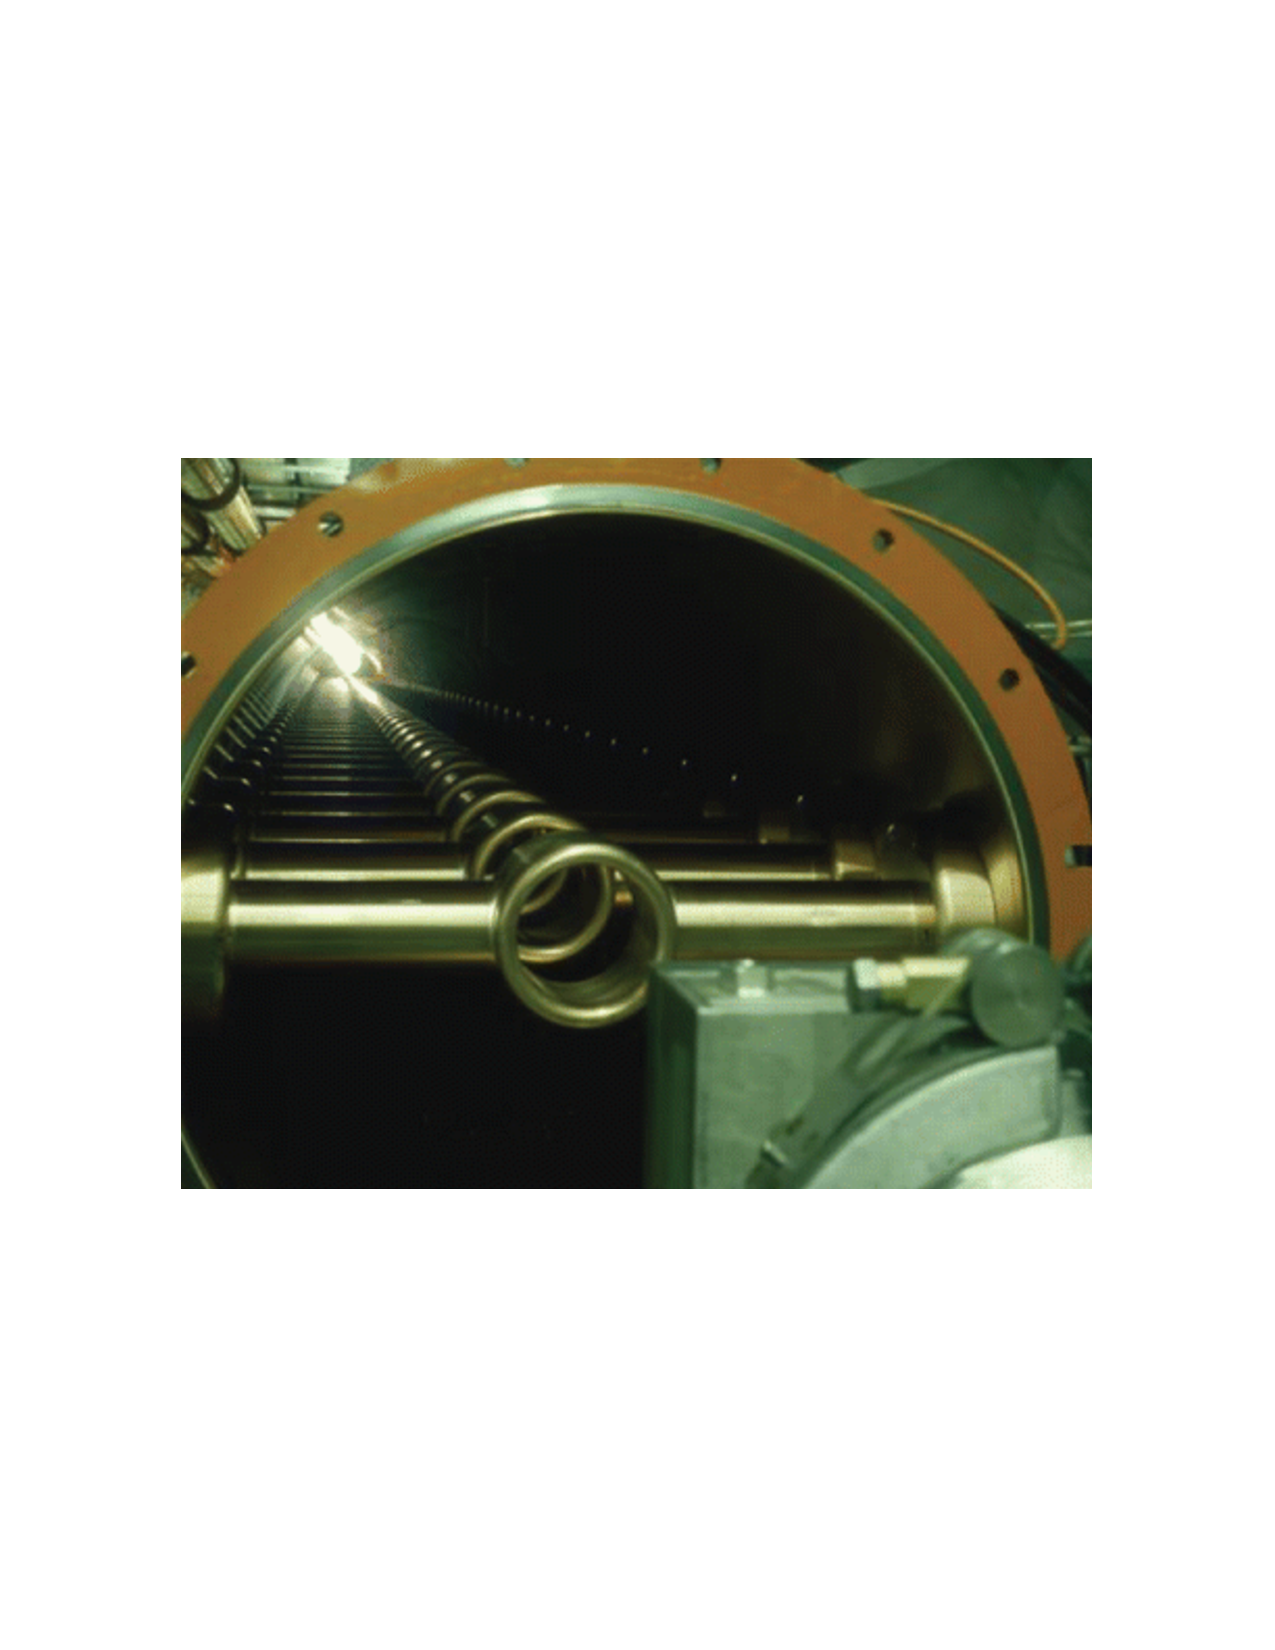
\includegraphics[width=\textwidth]{Figures/LHC_Diagrams/LHC__SPS__RFCavity_InsideView.pdf}
        \caption{The inside of the travelling wave guide structure,
          for the 200 MHz RF cavity in the SPS}\label{fig:sps_rf_inside}
      \end{subfigure}
       ~ %add desired spacing between images, e. g. ~, \quad, \qquad, \hfill etc.
      % (or a blank line to force the subfigure onto a new line)
      \begin{subfigure}[h]{0.45\textwidth}
        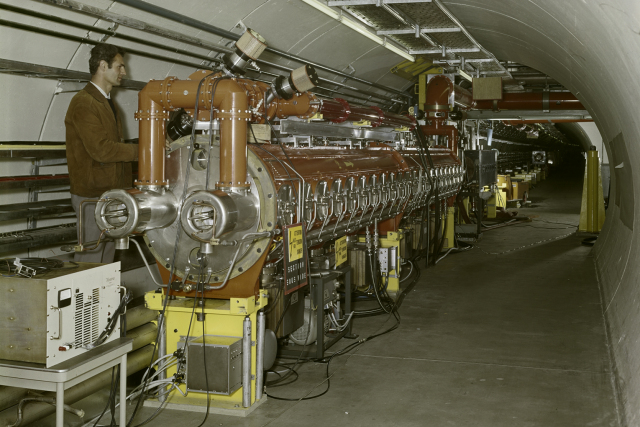
\includegraphics[width=\textwidth]{Figures/LHC_Diagrams/LHC__SPS__RFCavity_OutsideView.jpg}
        \caption{The outside of the 200 MHz RF cavity used to
          accelerate protons from 25 to 450 \GeV }\label{fig:sps_rf_outside}
      \end{subfigure}
       \caption{Features of the SPS, the fourth and final stage of
        the LHC injection chain}\label{fig:sps}
\end{figure}

\par Next, the protons arrive at the Super Proton Synchotron (SPS), where
they will be accelerated to 450 \GeV.  The SPS is the last stage of acceleration
before the protons are injected into the LHC.  The layout is show in
figure \ref{fig:sps}(\subref{fig:sps_layout}).  It has a circumference
of 7 km, and steers the proton beam with 744 dipole magnets, with 573
higher-order focusing magnets~\cite{LHC:LHC_sps_cern_website}.  Figure
\ref{fig:sps}(\subref{fig:sps_dipoles}) shows one of the dipole
mangets in the SPS tunnel.  Like all the other synchrotrons in the
injection chain, the acceleration is provided by RF cavities.  A 200
MHz system of RF cavities capture and fill the SPS by using 2-4
batches of 72 bunch proton beams from the
PS~\cite{LHC:TDR_Vol3_InjectionChain_Benedikt}.  Although the relative
change in frequency is small, the large degree of acceleration
necessitates the use of a tunable RF cavity.  The 200 MHz system has 2
sections of 4 travelling wave cavities in series, and another 2
sections of 5 cavities in series.  Figure
\ref{fig:sps}(\subref{fig:sps_rf_inside}) shows the insde of this
structure, which uses drift tubes to accelerate protons in the gaps
between tubes, with horziontally mounted bars, spaced 374
mm~\cite{LHC:LHC_SPS_200MHzRF_Dôme} apart, determining the periodicity
of the resonant RF field that builds up inside.  The outside of the
structure is shown in figure
\ref{fig:sps}(\subref{fig:sps_rf_outside}).  An additional 800 MHz
system is used to control the transverse emmitance.  It is also used
to stabalize the beam-line and prevent coupled-bunch
instabilities~\cite{LHC:TDR_Vol3_InjectionChain_Benedikt}.  

\par Finally, protons are injected into the LHC ring in one clockwise,
and another counter-clockwise rotating beams.  In order to work in the
limited space of the existing LEP tunnel, the two beams are contained
within a single meachanical and cryostate structure, with a dual-bore
design for each of the beams.  Here, each proton beam is
accelerated to their final energy of 7 \TeV, moving at 99.9999991$\%$
the speed of light, before they meet head on, producing 14 \TeV
center-of-mass collisions.  

\begin{figure}[h]
   \centering
  \includegraphics[width=0.8\textwidth]{Figures/LHC_Diagrams/LHC_Octant.jpg}
  \caption{The LHC ring is divided into eight octants} \label{fig:lhc_octants}
\end{figure}

\par The LHC ring itslef is divided into eight octants, with eight
straight sections that are located in front and behind each of the
eight collision points, where the beams are made to cross and
collide, as shown in figure \ref{fig:lhc_octants}.  These crossings
are known as interaction regions (IRs).  Four of these points are
currently being used by experiments.  TOTEM has detectors on either
side of the CMS experiment at one interaction region, known as point 5
(P5).  LHCf has detectors on either side of ATLAS at point 1 (P1).
MOeDAL has detectors near LHCb at point 8 (P8) and the ALICE detector
is located at point 2 (P2).  The following sections will cover the RF,
magnet, cryogen, and vaccuum technologies used in the LHC ring.  


\section{LHC Magnets}
\label{lhc_magnets}

\par Several types of magnets are used in order to properly circulate
and focus the proton beam as it makes its way around the 26.7 km long
tunnel.  A complete list of all types, can be found in the technical
design report~\cite{LHC:TDR_Vol1_MainRing_Brüning}, as well as through
CERN's outreach web
resources~\cite{LHC:LHC_outreach_listOfAllMagnets}.  This section will
give an overview of the a few of the critical subsystems: the septum
and kicker magnets used for injection from the SPS, the dipole mangets
used for bending the beam around the circumference of the ring, and
the higher-order-pole magnets that are used for focusing the beam.  

\begin{figure}[h]
   \centering
  \includegraphics[width=0.8\textwidth]{Figures/LHC_Diagrams/LHC_SingleTurnInjection.pdf}
  \caption{The single turn injection scheme.  A septum magnet makes
    the initial alignment.  The kicker magnet times the injection and
    makes the final alignment.  Bumper magnets align the LHC beam with
  the injected beam.} \label{fig:lhc_singleTurnInjection}
\end{figure}

\par The injection and extraction of proton beams from one synchrotron
to another involves three types of magnets, septums, kickers, and
bumpers.  Septum magnets contain a partition, or a septum, that
provides a boundary between a high magnetic field region and a
near-zero magnetic field region and are operated in DC or a
slow-pulsed mode~\cite{LHC:LHC_septums_Barnes}.  In case of injecting
a beam of protons into a synchrotron, the target beampipe of the synchrotron
passes through the low-field region, so the trajectory is unaffected
by the high-field region, which bends the injection beam towards the
synchroton alligning it horizontally, with the target beam.  The
kicker magnet, is a fast-pulsed magnet and provides the timing
selection in order to make a final bend vertical bend into the
synchrotron orbit, and into the correct basket of the synchroton bunch 
train~\cite{LHC:LHC_kickers_Barnes}.  Finally, bumper magnets make
small bends to the beam and align it with the injection site.  Figure
\ref{fig:lhc_singleTurnInjection} shows a schematic for this process,
where a transfer line brings protons to a septum, which bends the beam
to a kicker, which makes the final corrections to match the
synchrotron orbit.  For extraction, the kicker magnet quickly
displaces a portion of the beam, which is steered away by the septum,
while the original beam passes through it's low-field region 
unaffected.   

\begin{figure}[h]
   \centering
  \includegraphics[width=0.8\textwidth]{Figures/LHC_Diagrams/LHC_IR8-layout.pdf}
  \caption{Layout of Interaction Region 8, where one proton beam is
    injected into the LHC ring.  A transfer line from the SPS bring a
    proton in from the right.  In green, a septum magnet aligns the
    beam horizontally with the LHC.  In blue, a kicker magnet makes
    the final vertical alignment into the LHC, and is timed to fill
    one of the 400 MHz buckets of the RF capture
    system} \label{fig:lhc_IR8_layout}
\end{figure}

\begin{figure}[h]
   \centering
  \includegraphics[width=0.8\textwidth]{Figures/LHC_Diagrams/LHC_bunchStructure.pdf}
  \caption{The initial filling of 6 batches of protons from the PSB to
  the PS, leaves 12 empty buckets in the PS bunch structure.  The rise
time of the SPS magnet creates an additonal gap in the SPS bunch
structure.  Additional gaps emerge due to the rise time of the LHC
injection and dumping kicker magnets} \label{fig:lhc_bunchStructure}
\end{figure}

\par At the LHC, beam is injected at Interaction Regions (IR) 2 and
8~\cite{lhc:machine_description}.  Two transfer lines bring the beam
extracted from the SPS to $\sim150$ m of the LHC ring.  Five
Labertson-type septum magnets, of field strength $\sim1$ T, are used
to deflect each of the transfer line beams 12 mrad to align the
transfer beam horizontally with the LHC orbit.  Then, four $\sim0.12$T
MKI kicker magnets quickly deflect the beam 0.85 mrad to close the
obrit with the LHC ring.  Figure \ref{fig:lhc_IR8_layout} shows the
layout of the injection point at IR 8.  The green circle encloses the
septum structure, which provides the horizontal alignment, and the
blue encloses the kicker structure, which makes the final vertical
alignment and synchronizes the injection of the beam into the LHC.
The rise time for the field provided by the kicker magets in the LHC
and SPS determine the final bunch structure of the LHC.  Figure
\ref{fig:lhc_bunchStructure} extends figure
\ref{fig:ps}(\subref{fig:ps_splitting}) showing how the rise times of
the kickers that inject, or eject beam create gaps in the bunch
structure of the LHC.  The intial filling of the PS with 6 batches of
protons from the PSB, leaves one initial bucket unused in the PS.
After the splitting of the beam into the 25 ns bunches, there 12 empty
buckets at the of the PS bunch train.  The SPS is filled with three to
four of these trains, leaving an additional 8 25 ns buckets unfilled
due to the 220 ns rise time of the SPS kicker magnet. These three to
four trains are then injected into the LHC, where there are 38 or 39
bunch gaps due to the LHC injector 0.94 $\mu$s rise time.  At the end
of a full LHC orbit, 119 buckets are left empty to allow for the rise
time of the beam dumping kicker magnet, used to remove beam from the
LHC.     

\begin{figure}{h}
    \centering
    \begin{subfigure}[h]{0.450\textwidth}
        \includegraphics[width=\textwidth]{Figures/LHC_Diagrams/LHC_XSec_Dipole_Magnet__LHC-PHO-2001-187.jpg}
        \caption{Cross Section of a LHC dipole magnet}\label{fig:lhc_dipole_xs}
      \end{subfigure}
      ~ %add desired spacing between images, e. g. ~, \quad, \qquad, \hfill etc.
      % (or a blank line to force the subfigure onto a new line)
    \begin{subfigure}[h]{0.450\textwidth}
        \includegraphics[width=\textwidth]{Figures/LHC_Diagrams/LHC_Dipole_CollarAndCoils.jpg}
        \caption{A close-up picture of the non-magnetic collar and
          supercunducting coils of an LHC dipole magnet}\label{fig:lhc_dipole_collarAndCoils}
      \end{subfigure}
      ~ %add desired spacing between images, e. g. ~, \quad, \qquad, \hfill etc.
      % (or a blank line to force the subfigure onto a new line)
      \begin{subfigure}[h]{0.450\textwidth}
        \includegraphics[width=\textwidth]{Figures/LHC_Diagrams/LHC_Dipole_Field.pdf}
        \caption{A simulation of the homogenous, vertical magnetic field lines of the
          dipole. }\label{fig:lhc_dipole_field}
      \end{subfigure}
       ~ %add desired spacing between images, e. g. ~, \quad, \qquad, \hfill etc.
      % (or a blank line to force the subfigure onto a new line)
      \begin{subfigure}[h]{0.450\textwidth}
        \includegraphics[width=\textwidth]{Figures/LHC_Diagrams/LHC_Dipole_ExageratedCurvature.pdf}
        \caption{A diagram showing the exagerated curvature of a
          dipole magnet, with measurements for some of it's most
          important features. }\label{fig:lhc_dipole_curvature}
      \end{subfigure}
      \begin{subfigure}[h]{0.450\textwidth}
        \includegraphics[width=\textwidth]{Figures/LHC_Diagrams/LHC_Dipole_transp-2001-001_05.jpg}
        \caption{A $\sim$15 m long dipole magnet, in a staging area at
        CERN, awaiting installation}\label{fig:lhc_dipole_staging}
      \end{subfigure}
       \caption{Features of the dipole magnets used in the LHC}\label{fig:lhc_dipole}
\end{figure}

\par Once the beam is injected, the curved path around the
circumference of the LHC is maintained via 1232 superconducting dipole
magnets.  The superconducting material niobium-titanium, NbTi, is
cooled to 1.9 K in order to produce the 8.33 T field.  Figure
\ref{fig:lhc_dipole}(\subref{fig:lhc_dipole_xs}) shows a cross-section
view of one of the LHC dipoles.  The dual-bore design of the beam-pipe
is enclosed by an iron yoke, that serves as the cold mass to maintain
the superconducting temperature, and provides a 195 mm gap between
each beam.  A close up picture of the non-magnetic collar and
superconducting coils are shown in figure
\ref{fig:lhc_dipole}(\subref{fig:lhc_dipole_collarAndCoils}).  A
simulation  of the magnet in figure
\ref{fig:lhc_dipole}(\subref{fig:lhc_dipole_field}) shows the
homogenous, vertical magnetic field produced in the center of the
coil.  Diagram \ref{fig:lhc_dipole}(\subref{fig:lhc_dipole_curvature})
shows an exagerated view of the 2812 m radius curvature of each
dipole. However, since each dipole is only $\sim14$ m in length, this
curvature is hardly noticeable, as shown in a photo of an actual
dipole magnet in a staging area at CERN, awaiting installation in
figure \ref{fig:lhc_diple}(\subref{fig:lhc_dipole_staging}).   

\begin{figure}{h}
    \centering
    \begin{subfigure}[h]{0.450\textwidth}
        \includegraphics[width=\textwidth]{Figures/LHC_Diagrams/LHC_Quardupole_Schematic-1998-312.jpg}
        \caption{Cross Section of a LHC quadrupole magnet}\label{fig:lhc_quadrupole_xs}
      \end{subfigure}
      ~ %add desired spacing between images, e. g. ~, \quad, \qquad, \hfill etc.
      % (or a blank line to force the subfigure onto a new line)
    \begin{subfigure}[h]{0.450\textwidth}
        \includegraphics[width=\textwidth]{Figures/LHC_Diagrams/LHC_Quadrupole_TwinMagnets_Staged.jpg}
        \caption{A dual-bore quadrupole magnet, in a staging aread
          prior to installation}\label{fig:lhc_quadrupole_staged}
      \end{subfigure}
      ~ %add desired spacing between images, e. g. ~, \quad, \qquad, \hfill etc.
      % (or a blank line to force the subfigure onto a new line)
      \begin{subfigure}[h]{0.450\textwidth}
        \includegraphics[width=\textwidth]{Figures/LHC_Diagrams/LHC_Quadrupole_Focusing.png}
        \caption{A quadrupole magnet can provide focusing either in
          the horizontal or vertical direction}\label{fig:lhc_quadrupole_field}
      \end{subfigure}
       ~ %add desired spacing between images, e. g. ~, \quad, \qquad, \hfill etc.
      % (or a blank line to force the subfigure onto a new line)
      \begin{subfigure}[h]{0.450\textwidth}
        \includegraphics[width=\textwidth]{Figures/LHC_Diagrams/LHC_MultipoleFields.jpg}
        \caption{Multipole fields from a sextupole and an octupole magnet}\label{fig:lhc_multipole_field}
      \end{subfigure}
      \begin{subfigure}[h]{0.450\textwidth}
        \includegraphics[width=\textwidth]{Figures/LHC_Diagrams/LHC_MagneticCell.png}
        \caption{A typical 110m long magnetic cell at the LHC feturing
        several types of multipole magnets}\label{fig:lhc_magnetic_cell}
      \end{subfigure}
      ~ %add desired spacing between images, e. g. ~, \quad, \qquad, \hfill etc.
      % (or a blank line to force the subfigure onto a new line)
      \begin{subfigure}[h]{0.450\textwidth}
        \includegraphics[width=\textwidth]{Figures/LHC_Diagrams/LHC_InnerTriplet.pdf}
        \caption{Schematic of the Inner triplet structure that brings
          the two serarate beams together in the interagction region}\label{fig:lhc_inner_triplet}
      \end{subfigure}
      ~ %add desired spacing between images, e. g. ~, \quad, \qquad, \hfill etc.
      % (or a blank line to force the subfigure onto a new line)
      \begin{subfigure}[h]{0.450\textwidth}
        \includegraphics[width=\textwidth]{Figures/LHC_Diagrams/LHC_InteractionRegion.jpg}
        \caption{A simulation of two beams being squeezed together by
          the inner triplet.}\label{fig:lhc_beam_squeeze}
      \end{subfigure}
       \caption{Features of the dipole magnets used in the LHC}\label{fig:lhc_multipole}
\end{figure}


\par Quadrupole, septupole, octupole, and other multipole magnets are
used to focus a single beam, as well as squeeze the two beams
together.  There are 392 quadrupole magnets
on the LHC ring, each controlling the height and width of the beam.
Figure \ref{fig:lhc_multipole}(\subref{fig:lhc_quadrupole_xs}) shows a
schematic of a dual-bore quadrupole magnet, and figure
\ref{fig:lhc_multipole}(\subref{fig:lhc_quadrupole_staged}) shows an
actual quadrupole in a staging area before  installation.  Quadrupole
magnets use four sets of coils to create a magnetic field that either
squeezes the beam horizonally or vertically, as shown in figure
\ref{fig:lhc_multipole}(\subref{fig:lhc_quadrupole_field}). Finer
corrections to the beam shape are made with the multipole magnets,
since they are able to compress the beam from more than two axes.
Figure \ref{fig:lhc_multipole}(\subref{fig:lhc_multipole_field})
shows the fields lines of a sextupole and  octuple magnet.  A typical
cell of magnets, 110 m long, in the LHC beamline is shown in a diagram
in figure \ref{fig:lhc_multipole}(\subref{fig:lhc_magnetic_cell}), where the dipole, 
quadrupole and higher order magnet work in series to confine the
protons to the LHC ring.  Finally, a set of single bore magnets, known
as an inner triplet, bring the two beams together into an interaction
region.  Figure
\ref{fig:lhc_multipole}(\subref{fig:lhc_inner_triplet}) shows the
arrangement of magnets that squeeze the beam together, while figure
\ref{fig:lhc_multipole}(\subref{fig:lhc_beam_squeeze}) shows a
simulation of the beams being brought together to collide in the
interaction region.  


\section{LHC RF Technology}
\label{lhc_rf_overview}

\begin{figure}{h}
    \centering
    \begin{subfigure}[h]{0.450\textwidth}
        \includegraphics[width=\textwidth]{Figures/LHC_Diagrams/LHC_RFCavity_Schematic-1994-006.jpg}
        \caption{Cross section of a LHC superconducting Radio
          Frequency cavities, which accelerates the beam by imparting
          275 kW of power through a 400 MHz, 16 MV electric field
          resonanting in the cavity.}\label{fig:lhc_rf_xs}
      \end{subfigure}
      ~ %add desired spacing between images, e. g. ~, \quad, \qquad, \hfill etc.
      % (or a blank line to force the subfigure onto a new line)
    \begin{subfigure}[h]{0.450\textwidth}
        \includegraphics[width=\textwidth]{Figures/LHC_Diagrams/LHC_RFCavity_Staged.jpg}
        \caption{A picture of a four chamber RF cavity in a staging
          area, prior to installation}\label{fig:lhc_rf_staged}
      \end{subfigure}
      ~ %add desired spacing between images, e. g. ~, \quad, \qquad, \hfill etc.
      % (or a blank line to force the subfigure onto a new line)
      \begin{subfigure}[h]{0.450\textwidth}
        \includegraphics[width=\textwidth]{Figures/LHC_Diagrams/LHC_RFCavity_Installed.jpg}
        \caption{The four chamber RF cavity installed at Point 4 of
          the LHC}\label{fig:lhc_rf_at_p4}
      \end{subfigure}
      \caption{Features of the 400 MHz superconducting RF system used in the LHC}\label{fig:lhc_rf}
\end{figure}

\par The LHC uses a 400 MHz superconducting RF cavity system to
capture and accelerate the beam from 450 \GeV to 7
\TeV~\cite{lhc:machine_description}.  Two independent system are used
to provide 8 MV of RF voltage at injection at 16 MV during equilibrium
at 7 \TeV and deliver 275 kW of power to each beam.  This is provided
by 16 niobium sputtered cavities, housed in 4.5 K refrigeration units,
known as cryomodules, at Point 4 of the LHC octant.  The
superconducting material covering the inside of the cavity has
near-zero resistivity, which dissapates much less power and has a much
narrower resonance width, or Q-factor, than a cavity made from
normally conducting material. Figure
\ref{fig:lhc_rf}(\subref{fig:lhc_rf_xs}) shows a schematic of a four
cavity cryomodule.  The beam pipe passes through the center of each
chamber and longtitudinal (left to right in the diagram) electric
fields accelerate the protons each time they circulate the LHC
ring. Figure \ref{fig:lhc_rf}(\subref{fig:lhc_rf_staged}) shows an
actual four cavity module in a staging area prior to installation.  In
this picture, the resonance cavities are concealed underneath the
cyclidrical housing of the vacuum tank and cryostat.  Figure
\ref{fig:lhc_rf}(\subref{fig:lhc_rf_installed}) is a picture of the
module installed at Point 4.  The thin cylindrical structures
extending off the top is the LHe intake valve and quench system.  The
thicker cylindrical structures are the waveguides that couple the
cavities to the source of the electric field, the klystrons.   

\begin{figure}[h]
   \centering
  \includegraphics[width=0.8\textwidth]{Figures/LHC_Diagrams/LHC_KlystronBasic.pdf}
  \caption{A klystron uses a weak RF signal coupled to a resonace
    cavity to bunch an electron beam, which in turn creates an
    amplified RF signal as it passes through a second resonance cavity
    tuned to the same frequency.} \label{fig:lhc_klystron_operation}
\end{figure}

\par A Klystron is the source of RF power that builds up as a
resonance in the cavities that accelerate the protons.  Figure
\ref{fig:lhc_klystron_operation} shows a diagram of the basic
operating principle.  The device uses an anode to accelerate the
thermionic emission of electrons off of a cathode material into one or
more bunching cavities tuned to the frequency the device is designed
to produce.  This cavity is driven with a weak RF source, that groups
electrons into bunches.  Just as discussed for protons earlier, when
electrons arrive at the entrance of the cavity at just the right time,
it will experience the zero-point of the oscillation of the resonating
electric field.  If it arrives early or late, it is accelerated or
decelerated and thus bringing it closer to its neighbors, and
increasing the density of the beam.  After passing through multiple
chambers, the tightly bunched electrons enter a catcher cavity tuned
to the same resonance frequency.  As the electrons pass through at
this resonance frequency, standing electric waves are exicited and
quickly build up in the catcher cavity.  The electron beam is thus
used to amplify the original RF signal in the catcher cavity, which is
then transported via waveguide to power the RF cavity used to
accelerate the proton beamline.  

\begin{figure}[h]
   \centering
  \includegraphics[width=0.6\textwidth]{Figures/LHC_Diagrams/LHC_Klystron_Installed.jpg}
  \caption{One of sixteen 300 kW, 400 MHz klystrons that power the
    superconducting RF cavities that accelerate the proton beam.} \label{fig:lhc_klystron}
\end{figure}

\par At the LHC, 16 400 MHz, 300 kW kylstrons, work together to provide 4800 kW
of power to the superconducting RF
cavities~\cite{lhc:machine_description}.  They are also located at
Point 4, in the UX45 service cavern adjacent to the RF cavities, about
6 m below the beamline.  An average of 22 m of waveguide is used to
transport the power generated by the klystrons to the RF cavities.
Figure \ref{fig:lhc_klystron} shows a klystron installed at the LHC, and like most modern
klystrons, it also utilizes a multi-bunching chamber design.

\section{The LHC Cryogen System}
\label{lhc_cryogen_overview}

\begin{figure}[h]
   \centering
  \includegraphics[width=0.6\textwidth]{Figures/LHC_Diagrams/LHC_CoolingPlants.pdf}
  \caption{Layout of the five cryogenic islands, which are home to the
  eight facilities that provide liquid helium to the LHC} \label{fig:lhc_cryogenic_islands}
\end{figure}

\par The LHC is the largest cryogenic system in the
world~\cite{LHC:LHC_lhc_cryogen_cernWebsite}, as its operating
temperature is 1.8 K, in order to produce the high-magnetic fields
needed by the dipole magnets.  Addtionally, the acceleration,
mechanism, the RF cavities, are also superconducting, and must be
cooled to 4.5 K.  Over 120 tons of Helium are used as the cryogenic
medium, since once it is cooled below 2.17 K, it becomes a superfluid,
a phase of matter with a high thermal conductivity, making it ideal
for refridgeration.  Cryogenic and auxillary equipment are
concentrated into 5 \"cryogenic islands\" at Points 1,2,4,6, and
8~\cite{lhc:machine_description}.  As shown in figure
\ref{fig:lhc_cryogenic_islands}, Point 4,6, and 8 house two facilities
each, making a total of eight, one for each octant of the LHC arc. 

\begin{figure}{h}
    \centering
    \begin{subfigure}[h]{0.450\textwidth}
        \includegraphics[width=\textwidth]{Figures/LHC_Diagrams/LHC_Cryogen_4p5KFridgeCompressor.pdf}
        \caption{The compressor station for the 4.5 K refridgeration system}\label{fig:lhc_cryo_4p5_compressor}
      \end{subfigure}
      ~ %add desired spacing between images, e. g. ~, \quad, \qquad, \hfill etc.
      % (or a blank line to force the subfigure onto a new line)
    \begin{subfigure}[h]{0.450\textwidth}
        \includegraphics[width=\textwidth]{Figures/LHC_Diagrams/LHC_Cryogen4p5KFridge_Coldbox.pdf}
        \caption{The 4.5 K refridgeration system cold box, containing
          heat exchanging fins and turbins to cool the He}\label{fig:lhc_cryo_4p5_coldbox}
      \end{subfigure}
      \caption{Features of the 4.5 K refridgeration system}\label{fig:lhc_cryo_4p5}
\end{figure}

\par At each cryogenic plant, He is cooled to 80 K by cirulating it
through refridgeration equiptment with liquid nitrogen in the heat
exchangers\cite{LHC:LHC_lhc_cryogen_cernWebsite}.  Next, the He is
brough to 4.5 K with refridgerators recovered from the LEP experiment
\cite{LHC:LHC_cool_challenge}.  The He gas is first compressed and allowed
to expand, where it is cooled by losing energy through mechanical
turbo-expanders that run at up to 140,000 rpm on helium-gas
bearings.  Figure
\ref{fig:lhc_cryo_4p5}(\subref{fig:lhc_cryo_4p5_compressor}).  The He
is then liquified after passing through a vacuum sealed box containing
heat exchangers and more turbo-expanders
\cite{LHC:LHC_cryogenicHe_system_Lebrun}. The compressor for this
system is pictured in figure
\ref{fig:lhc_cryo_4p5}(\subref{fig:lhc_cryo_4p5_coldbox}).  Finally,
the liquified He is brought to 1.8 K with a refrigeration unit that
uses a cold compression train to decrease the saturation pressure, and
thus temperature as well. 

\begin{figure}[h]
   \centering
  \includegraphics[width=0.6\textwidth]{Figures/LHC_Diagrams/LHC_CryogenInTunnel.pdf}
  \caption{Cross section schematic of the cryogenic distribution
    system in the LHC tunnel} \label{fig:lhc_cryogen_tunnel_xs}
\end{figure}

\par In the LHC tunnel, a cryogenic distribution line runs parallel to
the machine \cite{LHC:LHC_cool_challenge}.  It consists of eight 3.2
km long cryostats, that contain the equipment to supply and recover
helium with temperatures ranging from 4 K to 75 K.  A total of 310
service modules, are used to control the system and provide safety
mechanisms against pressure buildup and magnet quenching.  Figure
\ref{fig:lhc_cryogen_tunnel_xs} shows a cross section of the cryogen
distribution system in the tunnel. 

\section{The LHC Vacuum System}
\label{lhc_vacuum_overview}

\par The LHC is also the largest operational vacuum system in the
world and is capable of achieving pressures lower than outer space
\cite{LHC:LHC_lhc_vacuum_cernWebsite}.  Three different types of
vacuum systems are used: one for insulating the helium distribution
lines, another for insulating the dipole magnets, and a final
ultra-high vacuum system for the beam pipe
\cite{lhc:machine_description}.  

\par The vacuum systems for insulating the helium distribution and
dipoles involves some 104 km of piping an over 250,000 welding
joints \cite{LHC:LHC_lhc_vacuum_cernWebsite}.  Pressure here is
required to be kept at $10^{-1}$ mbar, but at cryogenic temperatures,
pressuers tend to equalize at a much lower level, to $10^{-6}$ mbar
($\sim10^{-9}$ atm) \cite{lhc:machine_description}.   

\begin{figure}[h]
   \centering
  \includegraphics[width=0.6\textwidth]{Figures/LHC_Diagrams/LHC_BeamScreen.jpg}
  \caption{Beam screen for the LHC, with slits to allow for easy
    pumping of residual gas molecules in the beampipe.} \label{fig:lhc_beam_screen}
\end{figure}

\par The most stringent requirements come on the vacuum of the
beam-pipe.  The beam must minimize the number of interactions it has
with any particles outside of the interaction region.  A pressure of
$10^{-10}$ to $10^{-11}$ mbar are maintained in the 54 km of
beampipe \cite{LHC:LHC_lhc_vacuum_cernWebsite}.  Weeks of cryogenic
pumping, eventually condenses gas trapped in the beampipe into a
liquid that can be absorbed by the walls of the beampipe.  The inside
beampipe is also coated with a thin layer of a special substance 
developed at CERN, a titanium-zirconium-vanadium alloy, which absorbs
residual particles when heated.  780 ion pumps are used to remove the
noble gases and methane, which do not interact with the substance,
which acts as its own distributed pumping system.  Room-temperature
sections of the beampipe are also heated to 300$^{\deg}$ to be
baked-out from the outside.  This is done to periodically remove 
any material which may have settled and become trapped. Additionally,
the beam-pipe is designed with a racetrack shape, which optimises the
available aperture while leaving space for the cooling tubes, as shown
in figure \ref{fig:lhc_beam_screen}.  Slits also allow for gas
molecules to be easily pumped out from inside its volume.   


\chapter{The Compact Muon Solenoid}
\label{cms_description_overview}

The \acrfull{cms} is one of two general purpose detectors at the \acrshort{lhc}.  

\section{The Inner Tracker}
\label{inner_tracker_description}

\par The inner tracker is silicon and really really big, lots of
channels.

\section{The Electromagnetic Caliorimeter}
\label{ecal_description}

\par PBWO4 crystals.  APDs in the Barrel.  VPTs in the Endcaps

\subsection{Vacuum Photo-Triodes}
\label{vpt_description}

\par Extra time for VPTs

\subsection{Test Rig at UVa}
\label{vpt_test_rig_description}

\par Big maget, lots of light, test dem led's

\subsection{Results of UVa Tests}
\label{vpt_results_description}

\par Plots, Plots, plots, plots, plots

\section{The Hadronic Caliorimeter}
\label{hcal_description}

\par Brass, Steel, Soviet Sweat

\section{Forward Caliorimetry}
\label{fcal_description}

\par High eta, great for VBF

\section{Magnet and Return Yoke}
\label{magnet_description}

\par Describe solenoid and measuring field, and engineering marvel or
return yoke structure.

\section{Muon Chambers}
\label{muon_chamber_description}

\par APDs DTs and CSCs

\section{Data Collection Overview}
\label{data_collection_description}

\par L1 trigger, HLT etc


\chapter{Particle Reconstruction at CMS}
\label{reconstruction_overview}

\par Data is reconstructed at CMS using the $Particle Flow^{TM}$ algorithm

\section{Muon Reconstruction}
\label{muon_reco_overview}

\par Muons rely heavily on the inner tracker and muons chambers for
efficient identrification and reconstruction

\section{Electron Reconstruction}
\label{electron_reco_overview}

\par Electrons leave charged tracks in the inner tracker, and create a
wide shower of particles and thus energy deposits in the ECAL.  High
energy electrons sometimes traverse the entire distance of the ECAL
and leave energy in the HCAL, however the ratio of these two energies
is disproportionate for the ECAL, and thus this ratio is often used to
discriminate electrons from highly electromagnetic hadronic jets.

\section{Photon Reconstruction}
\label{photon_reco_overview}

\par Like electrons, but with no tracks, and narrower shower shape.

\section{Jet Reconstruction}
\label{jet_reco_overview}

\par Jets are formed by matching tracks from the inner tracker to
energy deposits in the ECAL and HCAL.  Energy clusters are identified
from the ECAL and HCAL, and everything is then clustered in a cone.

\section{Tau Reconstruction}
\label{tau_reco_overview}

\par So heavy that they decay to leptons or hadrons before traversing
the detector, they still leave an oddly-numbered pronged decay hadronically due
to charge conservation requiring that one of the hadrons produced be
eqaul charge to the tau.  This results in one charged, and any number
of neutral pions, or three charged, and any number of neutral pions. 

\section{Missing Transverse Energy Reconstruction}

\par since the detector is hermetic, and the tracker so granular, we
can ensure that no particles flew out of the detector due to lack of
coverage.  Only long-lived neutral particles can escape, such as
neutrinos in the standard model.  Many \acrshort{bsm} theories, such
as SUSY, are characterized by stable, neutral particles. 

\par MET is the vector sum of all of the tracks associated with a
particular primary vertex (? or all vertices in event).  Thus if there
wasa neutral particle that escaped detection, there would be a
momentum imbalance along the trajectory of that particle.  This is how
neutrinos are identified.  


\bibliographystyle{lucas_unsrt}
\bibliography{dissertation}
\printglossary[type=\acronymtype,title=List of Acronyms,toctitle=List of Acronyms]

\end{document}
